\documentclass[10pt,a4paper,spanish]{report}

\usepackage[spanish]{babel}
\usepackage[utf8]{inputenc}
\usepackage{amsmath, amsthm}
\usepackage{amsfonts, amssymb, latexsym}
\usepackage{enumerate}
% \usepackage[official]{eurosym}
\usepackage{graphicx}
\usepackage[usenames, dvipsnames]{color}
\usepackage[table]{xcolor}
\usepackage{colortbl}
\usepackage{multirow}
\usepackage{fancyhdr}
\usepackage[all]{xy}
% \usepackage{minted}
\usepackage{tikz}
\usepackage{pgfplots}
\usepackage{float}
\usepackage{cancel}
\pgfplotsset{compat=1.5}
\usepackage{picture}
\usepackage{subfigure}

\headsep 3mm
\skip\footins 16pt
\footskip 37pt


\usepackage[bookmarks=true,
            bookmarksnumbered=false, % true means bookmarks in
                                     % left window are numbered
            bookmarksopen=false,     % true means only level 1
                                     % are displayed.
            colorlinks=true,
            linkcolor=webblue]{hyperref}
\definecolor{webgreen}{rgb}{0, 0.5, 0} % less intense green
\definecolor{webblue}{rgb}{0, 0, 0.5}  % less intense blue
\definecolor{webred}{rgb}{0.5, 0, 0}   % less intense red

\newcommand{\HRule}{\rule{\linewidth}{0.5mm}} % regla horizontal para  el titulo

\pagestyle{fancy}
%con esto nos aseguramos de que las cabeceras de capítulo y de sección vayan en minúsculas

\renewcommand{\chaptermark}[1]{%
      \markboth{#1}{}}
\renewcommand{\sectionmark}[1]{%
      \markright{\thesection\ #1}}
\fancyhf{} %borra cabecera y pie actuales
\fancyhead[LE,RO]{{\bfseries\leftmark}}
\fancyhead[LO]{\bfseries Marta Gómez \& Braulio Vargas}
\fancyfoot[C]{\thepage{}}
\renewcommand{\headrulewidth}{0.5pt}
\renewcommand{\footrulewidth}{0pt}
\addtolength{\headheight}{0.5pt} %espacio para la raya
\fancypagestyle{plain}{%
      \fancyhead{} %elimina cabeceras en páginas "plain"
      \renewcommand{\headrulewidth}{0pt} %así como la raya
}

\usepackage[sfdefault,light]{roboto}  %% Option 'sfdefault' only if the base font of the document is to be sans serif
\usepackage[T1]{fontenc}

\setlength{\parindent}{0pt}
\setlength{\parskip}{1ex plus 0.5ex minus 0.2ex}

\usepackage{titlesec}

% \titleformat{\chapter}{\normalfont\huge\center}{--- \thechapter ---}{20pt}{}

\titleformat
{\chapter} % command
[display] % shape
{\Huge\center\bfseries} % format
{--- \thechapter ---} % label
{0.5ex} % sep
{
    \rule{\textwidth}{1pt}
    \vspace{1ex}
    \centering
} % before-code
[
\vspace{-0.5ex}%
\rule{\textwidth}{0.3pt}
] % after-code

\newcommand*{\titleGM}{\begingroup % Create the command for including the title page in the document
\hbox{ % Horizontal box
\hspace*{0.2\textwidth} % Whitespace to the left of the title page
\rule{1pt}{\textheight} % Vertical line
\hspace*{0.05\textwidth} % Whitespace between the vertical line and title page text
\parbox[b]{0.75\textwidth}{ % Paragraph box which restricts text to less than the width of the page

{\noindent\Huge\bfseries Fundamentos de \\[0.5\baselineskip] Redes}\\[2\baselineskip] % Title
{\large \textit{Curso 2015/2016}}\\[4\baselineskip] % Tagline or further description
{\Large Marta Gómez Macías\\Braulio Vargas López} % Author name

\vspace{0.5\textheight} % Whitespace between the title block and the publisher
{\htmladdnormallink{\includegraphics[width=2cm]{88x31.png}}
{http://creativecommons.org/licenses/by-nc/4.0/}\\
\texttt{Fundamentos de Redes by
\href{mailto:mgmacias95@gmail.com}{Marta Gómez Macías} \& \href{mailto:blackbrawl@gmail.com}{Braulio Vargas López}}
is licensed under a \htmladdnormallink{Creative Commons
Reconocimiento-NoComercial-CompartirIgual 4.0 Internacional License}
{http://creativecommons.org/licenses/by-nc/4.0/}}.}\\[\baselineskip] % Publisher and logo
}
\endgroup}


%Definimos autor y título
\title{\Huge Fundamentos de \\ Redes}
\author{Marta Gómez Macías}

% colores de capitulos
\definecolor{tema1}{rgb}{0.82, 0.1, 0.26}
\definecolor{tema2}{rgb}{0.0, 0.5, 1.0}
\definecolor{tema3}{rgb}{0.67, 0.38, 0.8}
\definecolor{tema4}{rgb}{0.0, 0.65, 0.31}

\begin{document}
\renewcommand{\tablename}{Tabla} 
\thispagestyle{empty}
\titleGM

\tableofcontents

\setcounter{chapter}{0}

\chapter{\textcolor{tema1}{Introducción a los Fundamentos de Redes}}
\section{\textcolor{tema1}Sistemas de comunicación y redes}

\input{sistemacom.latex}

Un \textit{\textcolor{tema1}{sistema de comunicación}} son todos los dispositivos y elementos que participan en la transmisión de información entre dos puntos remotos:
\begin{enumerate}[\color{tema1}{$\heartsuit$}]
  \item \textit{\textcolor{tema1}{Fuente}} o \textit{\textcolor{tema1}{emisor}}: origen de la información. En un teléfono, sería nuestra voz.
  \item \textit{\textcolor{tema1}{Destino}}: destinatario de la información transmitida.
  \item \textit{\textcolor{tema1}{Transmisor}}: intermediario entre el canal y el emisor, encargado de adaptar la señal transmitida a las características del medio de transmisión.
  \item \textit{\textcolor{tema1}{Receptor}}: intermediario entre el canal y el receptor, encargado de adaptar las características de la señal a las del destino.
\end{enumerate}

En el ejemplo de dos PC conectados a través de línea telefónica; los dos PCs son la fuente y el emisor, el canal de comunicación sería la red telefónica conmutada (RTC) y los elementos de transmisión y recepción, los módem necesarios para la conexión de los equipos a la RTC.

\begin{center}
\begin{tabular}{p{10cm}}
\hline
\textbf{\textcolor{tema1}{Información}}: conjunto de datos al que se dota de significado. Debemos diferenciar entre información como tal (contenido) y la señal que sirve de soporte a la misma (continente).\\
\hline
\end{tabular}
\end{center}

Un caso particular de los sistemas de comunicación son las \textit{\textcolor{tema1}{redes de computadores}}, cuyas características son:
\begin{enumerate}[\color{tema1}{$\longrightarrow$}]
  \item \textit{\textcolor{tema1}{Interconexión}}: la existencia de canales de transmisión permite la comunicación entre los equipos de la red.
  \item \textit{\textcolor{tema1}{Autonomía}}: los equipos son independientes en cuanto a funcionamiento, al contrario que en el concepto de \textit{\textcolor{tema1}{mainframe}} donde los equipos dependen de una unidad central. También se usa esta característica para distinguir las redes de computadores de los sistemas distribuidos.
  \item \textit{\textcolor{tema1}{Intercambio de información}}
\end{enumerate}

\subsection{\textcolor{tema1}Usos y clasificación de las redes}
El principal objetivo de las redes de computadores es el de \textit{\textcolor{tema1}{compartir recursos}}. Otras razones por las que se ha extendido su uso son:
\begin{enumerate}[\color{tema1}{$\diamondsuit$}]
  \item \textit{\textcolor{tema1}{Escalabilidad}}: Una red de computadores es más fácilmente escalable que un sistema supercomputador tradicional, pues la ampliación de éste podría requerir sustituir el equipo mientras que en una red bastaría con añadir nuevos equipos.
  \item \textit{\textcolor{tema1}{Seguridad}}: Al haber varios equipos cada uno con sus propias unidades de disco, memoria, etc., puede haber \textit{\textcolor{tema1}{duplicación de recursos}} lo que se traduce como un aumento de la seguridad.
  \item \textit{\textcolor{tema1}{Ahorro de costes}}: el mantenimiento y reparación de un supercomputador es mayor que el de un PC. El empleo de varias unidades sencillas frente a una sola compleja mejora la relación coste/prestaciones.
\end{enumerate}

Las redes de computadores se clasifican según dos criterios:
\begin{enumerate}[\color{tema1}{$\spadesuit$}]
  \item \textit{\textcolor{tema1}{Escala}}: depende de la distancia entre los equipos de la red. Puede ser:
  \begin{enumerate}[---]
    \item \textcolor{tema1}{LAN (\textit{Local Area Network})}: sólo se extiende hasta unos centenares de metros o unos pocos kilómetros.
    \item \textcolor{tema1}{MAN (\textit{Metropolitan Area Network})}: tiene los mismos fundamentos tecnológicos que una red LAN, pero se extiende una decenas de kilómetros (una ciudad). 
    \item \textcolor{tema1}{WAN (\textit{Wide Area Network})}: cubren todo un país o incluso un continente, llegando a alcanzar centenares o incluso miles de kilómetros.
  \end{enumerate}
  \item \textit{\textcolor{tema1}{Tecnología de transmisión}}: existen dos formas destacadas de llevar a cabo la comunicación entre los equipos de una red:
  \begin{enumerate}[---]
    \item \textcolor{tema1}{\textit{Difusión}}: existe un único medio de transmisión, compartido por todos los equipos, sobre el que se realizan todas las transmisiones.
    \item \textcolor{tema1}{\textit{Punto a punto}}: enlaces entre dos equipos en los que unas veces hacen de receptor y otras de emisor. En contraposión a éstas, las anteriores se denominan \textit{\textcolor{tema1}{multipunto}}.
  \end{enumerate}
\end{enumerate}

Cuando el número de enlaces es igual al número de parejas posibles de equipos, se habla de una \textit{\textcolor{tema1}{topología}} completamente conectada, pero no es usual debido a su alto coste.

\input{tectrans.latex}
\label{tectrans}


Las redes LAN usan tecnología de Difusión y las WAN, punto a punto.

En la estructura de una red de computadores se diferencian los siguientes elementos:
\begin{enumerate}[\color{tema1}{$\clubsuit$}]
  \item \textit{\textcolor{tema1}{Host}}: son los sistemas finales de usuario.
  \item \textit{\textcolor{tema1}{Subred}}: conjunto de elementos que interconectan a los \textit{\textcolor{tema1}{host}}. Ésta está compuesta por:
  \begin{enumerate}[---]
    \item \textit{\textcolor{tema1}{Líneas de transmisión}}: enlaces de comunicación
    \item \textit{\textcolor{tema1}{Nodos de comunicación}}: Dispositivos que transportan datos desde un origen a un destino dados.
  \end{enumerate}
\end{enumerate}

\input{redcom.latex}

\section{\textcolor{tema1}Diseño y estandarización de redes}

Cuando planteamos el diseño de una red de computadores tenemos que solucionar problemas como la transmisión de bits, acceso al medio de transmisión, control de errores, etc., con el fin de conseguir una comunicación eficaz entre los equipos involucrados.

Para simplificar esta tarea, se aborda el diseño en \textit{\textcolor{tema1}{capas}}. Así obtendremos un sistema modular y más flexible. Al conjunto de capas denifido y sus funciones se les denomina \textit{\textcolor{tema1}{modelo de referencia}}. 

Los modelos de red son estándares y hay dos tipos:
\begin{enumerate}[\color{tema1}{$\triangle$}]
  \item \textit{\textcolor{tema1}{de facto}}: han sido adoptados sin haber seguido un proceso de estandarización formal.
  \item \textit{\textcolor{tema1}{de jure}}: han sido desarrollados por organismos de estandarización reconocidos.
\end{enumerate}

Los modelos más conocidos son \textit{\textcolor{tema1}{OSI}} y \textit{\textcolor{tema1}{TCP/IP}}.

\begin{center}
\input{estandar.latex}
\label{estandar}
\end{center}

El modelo OSI se define en siete capas, que de abajo a arriba son:
\begin{enumerate}[\color{tema1}{$\bigstar$}]
  \item \textit{\textcolor{tema1}{Física}}: En ella se llevan a cabo funciones relacionadas con la transmisión de datos desde el punto de vista de la gestión de características eléctricas, mecánicas y funcionales para una adecuada transferencia sobre el canal. Sería la tarjeta de red.
  \item \textit{\textcolor{tema1}{Control del enlace de datos}}: los bits de datos se agrupan en bloques llamados \textit{\textcolor{tema1}{tramas}}, tiene tres funciones:
  \begin{enumerate}[(a)]
    \item delimitación de tramas, para conocer el principio y el fin de un bloque de datos y sincronizar al emisor y al receptor
    \item control de errores, para conseguir que la información recibida se corresponda con la enviada
    \item control de flujo, para evitar que el emisor sature el \textit{\textcolor{tema1}{buffer}} de recepción del destino debido a una velocidad u ocupación diferente de las dos partes.
  \end{enumerate}
  \item \textit{\textcolor{tema1}{Red}}: Tiene tres funciones principales:
  \begin{enumerate}[(a)]
    \item encaminamiento, cuyo objetivo es el establecimiento de la ruta (secuencia de líneas y nodos de conmutación en la subred) a seguir desde un origen hasta un destino.
    \item control de congestión, evita la saturación de la capacidad de la subred como consecuencia de un elevado tráfico. 
    \item interconexión de redes, posibilita la transmisión de datos entre estaciones finales situadas en redes distintas.
  \end{enumerate}
  \item \textit{\textcolor{tema1}{Transporte}}: controla lo mismo que la capa de enlace de datos pero, a diferencia de ésta, sólo lo controla entre los dos hosts, es decir, controla que la transmisión de datos entre los dos hosts se haga correctamente. Otra función de esta capa es la de multiplexar aplicaciones sobre una misma conexión de red.

  \item \textit{\textcolor{tema1}{Sesión}}: esta capa se encarga de gestionar el ``turno de palabra'' en una comunicación entre los hosts participantes.

  \item \textit{\textcolor{tema1}{Presentación}}: en esta capa se abordan la representación de datos que provienen de la capa superior (por ejemplo a través de cifrado o codificación). Esta capa resuelve heterogeneidades respecto de la diferente representación interna de la información en cada uno de los hosts extremos.

  \item \textit{\textcolor{tema1}{Aplicación}}: servicios finales que se ofrecen al usuario: skype, dropbox, correo electrónico, etc.
\end{enumerate}

El modelo OSI tiene capas con muy poco contenido, por eso, en otros modelos se emplea un número menor de capas mediante trasvase de funciones asociadas a otros niveles. En TCP/IP (el modelo que se usa en internet) hay sólo tres capas:

\begin{enumerate}[\color{tema1}{$\bigstar$}]
  \item \textit{\textcolor{tema1}{Aplicación}}: servicios de usuario como \textit{\textcolor{tema1}{telnet}} (acceso remoto), \textit{\textcolor{tema1}{ftp}} (transferencia de ficheros), \textit{\textcolor{tema1}{smtp}} (correo electrónico), \textit{\textcolor{tema1}{http}} (web), etc.
  \item \textit{\textcolor{tema1}{Transporte}}: control de flujo, de errores, de congestión y de conexión (extremo a extremo)
  \item \textit{\textcolor{tema1}{Red}}: función de encaminamiento.
\end{enumerate}

TCP/IP es una red software, ya que puede implementarse sobre cualquier tecnología de red sin ser dependiente de ella, por ello, TCP/IP es el modelo más extendido en la actualidad y un ejemplo de \textit{\textcolor{tema1}{de facto}}. ¿Por qué en TCP/IP no se considera la red subyacente como parte del modelo? Porque TCP/IP es software estándar, pero la red subyacente puede variar en cada ordenador.%, por tanto tendríamos que hacer una versión de TCP/IP para cada tipo de hardware que existiese y eso no es lo que se quiere. 


\newpage
\section{\textcolor{tema1}Terminología y servicios}
\begin{center}
\input{comosi.latex}
\label{comosi}
\end{center}

Dadas dos capas adyacentes $N$ y $N+1$, la capa inferior se denomina \textit{\textcolor{tema1}{proveedora de servicios}} y la superior \textit{\textcolor{tema1}{usuaria de servicios}}, ya que la capa $N$ ofrece una serie de \textit{\textcolor{tema1}{servicios}} transparentes a $N+1$.

Los elementos hardware o software de una capa se conocen como \textcolor{tema1}{\textit{entidades de nivel} $N$}. Las entidades de nivel $N$ en el emisor y en el receptor se llaman \textit{\textcolor{tema1}{entidades pares}} o \textit{\textcolor{tema1}{paritarias}}, ya que se conectan dos a dos.

Hay dos tipos de comunicación entre el emisor y el receptor:

\begin{enumerate}[\color{tema1}{$\heartsuit$}]
  \item \textit{\textcolor{tema1}{Real}} o \textit{\textcolor{tema1}{Vertical}}: flujo que sigue la información entre el emisor y el receptor: intercambio de datos entre capas adyacentes, en sentido descendente (aplicación a física) en el emisor y ascendente (física a aplicación) en el receptor.
  \item \textit{\textcolor{tema1}{Virtual}} u \textit{\textcolor{tema1}{Horizontal}}: comunicación entre entidades paritarias. Para hacer una función se necesita la colaboración de las entidades pares emisora y receptora. Por eso en cada capa (menos en la física) se añade una cabecera para ayudar a comunicar a las partes involucradas.
\end{enumerate}

En relación con la comunicación horizontal, un \textit{\textcolor{tema1}{protocolo}} es el conjunto de reglas y convenciones que se tienen que aplicar en una comunicación entre dos entidades. A las capas y protocolos asociados se les denominan \textit{\textcolor{tema1}{arquitectura de red}}. En este sentido $OSI$ no es una arquitectura porque no se definen los protocolos, mientras que $TCP/IP$ sí es una arquitectura, ya que en cada capa se conocen los protocolos que se tienen que tener en cuenta. La especificación en capas de una arquitectura de red se conoce como \textit{\textcolor{tema1}{pila de protocolos}}.

Respecto a la comunicación vertical de las capas se realiza mediante la \textit{\textcolor{tema1}{interfaz}}, más concretamente con \textit{\textcolor{tema1}{los puntos de acceso (Service Access Points; SAP)}}. Dentro de la información que se transmite en los SAP se distinguen la \textit{\textcolor{tema1}{unidad de datos de servicio (Service Data Unit; SDU)}} son los datos que se manejan por la entidad (los que se quieren enviar) y vienen de la capa superior; y la \textit{\textcolor{tema1}{unidad de datos de protocolo (Protocol Data Unit; PDU)}} que es la cabecera añadida para llevar a cabo las operaciones desarrolladas con las entidades paritarias. A continuación se puede ver cómo actúan todos estos conceptos:

\begin{center}
  \input{interfazSAP.latex}
  \label{interfazSAP}
\end{center}

\subsection{\textcolor{tema1}Retardo en la comunicación}
Se refiere al tiempo que tarda la información en llegar desde el nodo destino al origen (\hyperref[retardos]{Figura \ref*{retardos}}).
\begin{figure}[!h]
  \centering
  \includegraphics[width=0.7\textwidth]{retardos}
  \caption{Retardos en la transmisión de un paquete}
  \label{retardos}
\end{figure}

El tiempo de \textit{\textcolor{tema1}{transmisión}} es el tiempo que se tardan en transferir todos los bits a la red:

\begin{displaymath}
  T_t = \frac{Tam (B)}{Velocidad_{transmision} (bps)}
\end{displaymath}

El tiempo de \textit{\textcolor{tema1}{propagación}} es el tiempo que tarda en llegar la información al destino:

\begin{displaymath}
  T_p = \frac{Distancia (m)}{Velocidad_{procesamiento} (m/s)}
\end{displaymath}

Y el tiempo de \textit{\textcolor{tema1}{procesamiento}} es el tiempo que tarda el nodo destino en procesar la información recibida.


\subsection{\textcolor{tema1}Servicios}
Los servicios que ofrece cada una de las capas pueden ser:

\begin{enumerate}[\color{tema1}{$\heartsuit$}]
  \item \textit{\textcolor{tema1}{Orientado a conexión}}: caracterizado por el hecho de establecerse una conexión como paso previo a la transmisión de datos entre el emisor y el receptor. Esta conexión se realiza enviando un paquete de un tamaño por parte del host emisor que el host receptor debe devolver. Cuando se ha devuelto, comienza el envío del resto de paquetes con la información a enviar. Se hace cuando sí importa que la información que se envía llegue al receptor.

\begin{figure}[!h]
  \begin{center}
    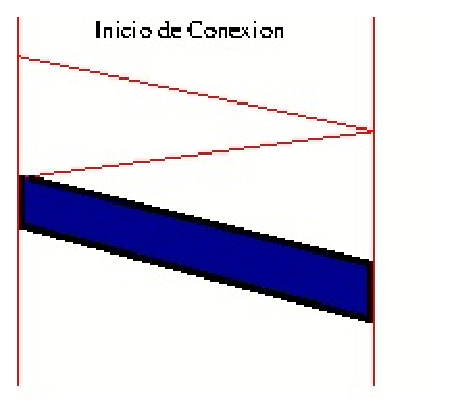
\includegraphics[width=0.4\textwidth]{iniconec}
  \end{center}
\end{figure}
  \item \textit{\textcolor{tema1}{No orientado a conexión}}: en este caso, no se necesita que haya una conexión entre los hosts previa, sino que el envío de información se haga con mucha rapidez. Un ejemplo de esto es la reproducción on-line de vídeos, donde no importa si se pierde un $frame$ o dos, sino que lleguen los paquetes lo más rápido posible para que dé sensación de fluidez.
  \item \textit{\textcolor{tema1}{Confirmado}}: el host emisor tiene constancia de que al host receptor le ha llegado el paquete enviado.
  \item \textit{\textcolor{tema1}{No confirmado}}: lo contrario al anterior.
\end{enumerate}

Por ejemplo, una carta es un servicio no orientado a conexión, ya que al echar la carta al buzón ya nos olvidamos de ella. En cambio, una llamada telefónica es un servicio orientado a conexión, porque antes de iniciar la comunicación debe establecerse una conexión entre ambas partes y finalmente una desconexión.

\section{\textcolor{tema1}Internet: Arquitectura y Direccionamiento}

\subsection{\textcolor{tema1}Arquitectura}
Existen varios tipos de red, estableciendo una topología jerárquica:

\begin{enumerate}
  \item \textit{\textcolor{tema1}{Intranets (Ethernet) del usuario}}: zona pública+zona privada. Se refieren a las redes locales de cada usuario donde se incluyen direcciones privadas para su subred local y direcciones públicas para acceder a la red.
  \item \textit{\textcolor{tema1}{Redes de acceso}}: xDSL (toda la familia DSL, por ejemplo, ADSL), RDSI, FTTH (Fibre To The Home (fibra óptica)), etc del ISP.
  \item \textit{\textcolor{tema1}{Redes troncales}}: ATM, SDH, SONET, etc$\ldots$ de grandes operadores de telecomunicaciones. Un ejemplo de red troncal sería la \textit{\textcolor{tema1}{red iris}}, que conecta a la comunidad investigadora y las distintas universidades en España. Hay varios tipos de redes troncales, según su tamaño: \textit{\textcolor{tema1}{Tier-1}}, \textit{\textcolor{tema1}{Tier-2}} y \textit{\textcolor{tema1}{Tier-3}}.
\end{enumerate}

Los \textit{\textcolor{tema1}{puntos neutros}} son puntos en los cuales las distintas redes ISP se interconectan para intercambiar tráfico.

\subsection{\textcolor{tema1}Direccionamiento}
Cuando queremos acceder a una página web, se forma un paquete de datos con una determinada información en las distintas capas que se iban trasmitiendo entre los distintos nodos a través de internet hasta llegar al destino, devolviendo la información requerida.

El direccionamiento, dependiendo de la capa, se hace de distintas formas:
\begin{enumerate}[\color{tema1}{$\heartsuit$}]
  \item \textit{\textcolor{tema1}{Nombre de dominio}}: En la capa de aplicación, para direccionar se usa el nombre de dominio debido a que la capa de aplicación es justo la que interacciona con nosotros y un nombre de dominio es más fácil de recordar. La capa lo traduce a direcciones IP que entiende la máquina.

  \item \textit{\textcolor{tema1}{Dirección IP}}: se localiza en la capa de red e identifica a los host (tanto fuente como destino).

  \item \textit{\textcolor{tema1}{Puertos}}: un puerto sirve para contestar peticiones que nos envíen otros dispositivos. Hay puertos de propósito específico, dinámicos, etc. Se localizan en la capa de transporte.
\end{enumerate}

Hay dos tipos básicos de direcciones IP:
\begin{enumerate}[\color{tema1}{$\bigstar$}]
  \item \textit{\textcolor{tema1}{Públicas}}: sólo direcciona a un dispositivo y se paga (o se alquila) por ella. Son unívocas, cada dirección se asigna sólo a un dispositivo en internet.

  \item \textit{\textcolor{tema1}{Privadas}}: funcionan como un número de teléfono en una centralita. Son direcciones que se pueden repetir en el mundo, pero dentro de una red privada serán únicas (y fuera de ella lo serán si se suman a la IP del router). Cuando se abre un canal hacia una página web, la IP que aparece es la de nuestro router. Su razón de existencia se debe a que sin ellas, habríamos agotado hace ya mucho tiempo el número de dispositivos máximos que podemos conectar a internet.
\end{enumerate}

Los rangos reservados para IPs privadas son:
\begin{enumerate}[\color{tema1}{$\clubsuit$}]
  \item \textit{\textcolor{tema1}{10.0.0.0/8}}: permiten tener $2^{24}$ dispositivos conectados. Se usan en redes muy grandes y abarcan desde 10.0.0.0 a 10.255.255.255
  \item \textit{\textcolor{tema1}{172.16.0.0/11}}: son para redes intermedias, como la red de la UGR. Abarcan desde 172.16.0.0 a 172.31.255.255
  \item \textit{\textcolor{tema1}{192.168.0.0/16}}: son para redes pequeñas, 16 veces más pequeñas que las anteriores. Abarcan desde 192.168.0.0 a 192.168.255.255
\end{enumerate}

\section{\textcolor{tema1}Cuestiones y ejercicios}
\textbf{7. ¿Cuál es el tiempo necesario para enviar un paquete de 1000 Bytes, incluidos 50 Bytes de cabecera, por un enlace de 100 Mbps y 10 Km?}

El retardo de transmisión será igual a:

\begin{displaymath}
  T_t = \frac{1000 B \cdot 8 \frac{b}{B}}{100 Mbps} = 80 \mu s
\end{displaymath}

Y el de propagación:

\begin{displaymath}
  T_p = \frac{10 Km \cdot 1000 \frac{m}{Km}}{2 \cdot 10^8 m/s} = 50 \mu s
\end{displaymath}

Y el tiempo total para enviar el paquete será la suma de ambos:

\begin{displaymath}
  T_{total} = T_p + T_t = 130 \mu s
\end{displaymath}

\chapter{\textcolor{tema2}{Servicio y protocolos de aplicación en internet}}

\section{\textcolor{tema2}Introducción a las aplicaciones de red}
\subsection{\textcolor{tema2}Estructura de protocolos}
\input{pila.latex}

En el esquema, vemos la pila de protocolos de TCP/IP, aunque falta HTTP. Entre los más destacados están:
\begin{enumerate}[\color{tema2}{$\longrightarrow$}]
  \item \textit{\textcolor{tema2}{SMTP}}: para correo electrónico
  \item \textit{\textcolor{tema2}{FTP}}: para transferir archivos
  \item \textit{\textcolor{tema2}{TELNET}}: conexión entre una máquina y otra para administración remota
  \item\label{protocolosnmp} \textit{\textcolor{tema2}{SNMP}}: para gestión de la red
  \item \textit{\textcolor{tema2}{HTTP}}: el protocolo de la web
  \item \textit{\textcolor{tema2}{TCP}}: protocolo que nos proporciona una conexión fiable
  \item \textit{\textcolor{tema2}{UDP}}: protocolo más ``ligero'' para una ejecución más eficiente, pero con menos funcionalidad que TCP.
  \item \textit{\textcolor{tema2}{IP}}: el protocolo más importante de la capa de internet
  \item \textit{\textcolor{tema2}{ICMP}}: también para gestión de redes
  \item \textit{\textcolor{tema2}{EGP}}: su principal uso es calcular la dirección destino
  \item \textit{\textcolor{tema2}{ARP}}: su principal uso es calcular direcciones MAC.
\end{enumerate}

\subsection{\textcolor{tema2}Arquitectura Cliente/Servidor}
Un \textit{\textcolor{tema2}{servidor}} es una aplicación que permite el acceso remoto a ciertos recursos software o hardware en un \textit{\textcolor{tema2}{host}}. La aplicación servidora está siempre en escucha hasta que le llega alguna solicitud remota por parte de un \textit{\textcolor{tema2}{cliente}}.

Ambos, tanto cliente como servidor, tienen unas características muy diferentes entre sí. El servidor debe estar siempre en funcionamiento para poder estar siempre a la escucha de peticiones, debe tener una IP permanente y pública para que sea fácil de localizar y, sobre todo en grandes ``data centers'' suelen estar agrupados en granjas.

Por otro lado, los clientes funcionan intermitentemente, no tienen por qué estar pagando una IP permanente para su router por lo que ésta suele ser dinámica, y al acceder desde un dispositivo distinto al router también suelen tener IP privada. Los clientes son los que inician la comunicación con el servidor y no se comunican entre sí, menos en las \textit{\textcolor{tema2}{redes P2P}} donde las máquinas que intervienen en la comunicación son ``iguales''.

\subsection{\textcolor{tema2}Sockets}
Los \textit{\textcolor{tema2}{sockets}} son una forma de comunicación con una especie de API o interfaz, por así decirlo, que utilizan los procesos para comunicarse entre sí de forma segura. Para esta comunicación, se le asigna al socket un \textit{\textcolor{tema2}{puerto}}. Por tanto, un \textit{\textcolor{tema2}{socket}} es un proceso o hilo existente en la máquina cliente y en la máquina servidora, que sirve en última instancia para que el programa servidor y el cliente lean y escriban la información. Esta información será la transmitida por las diferentes capas de red. En la práctica, es un puntero a una estructura.

\input{socket.latex}

Los procesos envían y reciben mensajes a/desde su socket. Para recibir mensajes, un proceso debe tener un \textit{\textcolor{tema2}{identificador}} (IP + puerto).

Los servidores se pueden identificar por su dirección IP y por el puerto 80. Esto se conoce como \textit{\textcolor{tema2}{puertos bien conocidos}} o \textit{\textcolor{tema2}{definidos}}, ya que todo el mundo sabe para qué se usan y cuáles son. Podemos no usar el puerto 80 para nuestro servidor web, pero entonces, debemos identificar qué puerto es el que usamos.

\subsection{\textcolor{tema2}Retardo en cola}
El \textit{\textcolor{tema2}{tiempo de servicio}} es el tiempo medio en dar servicio a un solicitante (desde que éste envía la petición hasta que obtiene una respuesta). Sirve tanto para páginas como para routers, que hacen un servicio de reenvío al solicitante.

Para estimar los retardos (tiempos) en cola se usa la \textit{\textcolor{tema2}{teoría de colas}}. %El servidor se modela mediante un sistema $M/M/1$, ya que sólo tenemos un único servidor

\input{retardocola.latex}

El retardo en cola se calcula mediante la siguiente expresión:
\begin{displaymath}
R = \frac{\lambda \cdot (T_s)^2}{1 - \lambda \cdot T_s}
\end{displaymath}

donde $T_s$ es el tiempo de servicio y $\lambda$ el ratio de llegada de solicitudes.

Tanto el \textit{\textcolor{tema2}{ratio de llegada ($\lambda$)}} como el \textit{\textcolor{tema2}{tiempo de servicio ($T_s$)}} siguen una distribución normal o de Poisson.

Con esta ecuación podemos medir el retardo teniendo en cuenta el tiempo promedio que se tarda en dar a un solicitante una respuesta ($T_s$) y el número de solicitantes que hay ($\lambda$). El resultado de esta ecuación nos devuelve un resultado en segundos.

Si analizamos la expresión, vemos que hay casos en los que nos da un resultado a interpretar:
\begin{enumerate}[\color{tema2}{$\heartsuit$}]
  \item En el caso de que $\lambda \cdot T_s$ sea mayor que $1$, ya que nos saldría un retardo negativo. Esto quiere decir que tenemos una congestión muy grande en nuestra red.
  \item En el caso de que $\lambda \cdot T_s$ tienda a $1$, nuestro retardo tiende a $\infty$.
\end{enumerate}

En ambos casos, lo más seguro es que tengamos una congestión en nuestra red, nos llegan más solicitudes de las que podemos atender.

Para que nuestro servicio sea rentable, el tiempo de servicio tiene que ser menor que el ratio de llegada ($T_s < \lambda$).

Esta misma expresión se puede usar para calcular el retardo en cola en un router.

\subsection{\textcolor{tema2}{¿}Qué definen los protocolos de aplicación?}
Un protocolo se encuentra definido por:
\begin{enumerate}[\color{tema2}{$\triangle$}]
  \item \textit{\textcolor{tema2}{Tipos de servicios}} que ofrece, por ejemplo, de correo electrónico, de envío de ficheros, etc.
  \item \textit{\textcolor{tema2}{Tipos de mensajes}} los ejemplos más tipicos de mensajes son de petición (request) y respuesta (response).
  \item \textit{\textcolor{tema2}{Sintaxis}}, que está definida por la estructura de ``campos'' en el mensaje, es decir, debe tener un formato:

  \input{protocolo.latex}

  \item \textit{\textcolor{tema2}{Semántica}}, se refiere al significado de dichos ``campos''.
  \item \textit{\textcolor{tema2}{Reglas}}, se refiere a cuándo los procesos envían/responden a mensajes. Para que la comunicación sea efectiva debe hacerse siguiendo unas reglas.
\end{enumerate}

Hay varios tipos de protocolos. Los dos más importantes son:
\begin{enumerate}[\color{tema2}{$\diamondsuit$}]
  \item \textit{\textcolor{tema2}{Protocolos de dominio público}}: están definidos en los RFCs\footnote{Request for comments, este tipo de protocolos buscan la colaboración/feedback de la gente para encontrarle fallos o mejorarlos}. Normalmente buscan ser estándarizados. Por ejemplo HTTP,  SMTP, etc.
  \item \textit{\textcolor{tema2}{Protocolos propietarios}}: al contrario que los de dominio público, son creados por una empresa e impantados en un producto. Estas empresas intentan esconderlo lo máximo posible para que nadie sepa cómo funciona el protocolo.
\end{enumerate}

Además hay otras clasificaciones, aunque menos importantes:
\begin{enumerate}[\color{tema2}{$\diamondsuit$}]
  \item \textit{\textcolor{tema2}{In-band versus out-of-band}}: Los protocolos \textit{\textcolor{tema2}{In-band}} mandan en el mismo paquete la información completa, tanto de datos como de control (HTTP) y los protocolos \textit{\textcolor{tema2}{Out-of-band}}, usan canales distintos para cada cosa (FTP). Por ejemplo, FTP envía la información de control (usuario, contraseña, comandosget/post, etc) por una conexión y los datos, por otra conexión paralela separada.
  \item \textit{\textcolor{tema2}{stateless versus state-full}}: Los protocolos \textit{\textcolor{tema2}{stateless}} no guardan información del cliente, a no ser que tengan una intranet o un fichero como las cookies. Los protocolos \textit{\textcolor{tema2}{state-full}} son servicios que guardan el estado del cliente, por ejemplo, el carrito de la compra, si eres premium o no...
  \item \textit{\textcolor{tema2}{persistentes versus no-persistentes}}: Los protocolos \textit{\textcolor{tema2}{persistentes}} siempren están conectados mientras que los \textit{\textcolor{tema2}{no-persistentes}}, crean una conexión cada vez que se manda un trocito de información.
\end{enumerate}

\subsubsection{\textcolor{tema2}Tendencia: hacer los protocolos flexibles}
La tendencia hoy en día, para no trabajar con cabeceras muy grandes, es hacer \textit{\textcolor{tema2}{cabeceras flexibles}}, es decir, poner una cabecera fija muy pequeñita y luego añadir trozos (\textit{\textcolor{tema2}{chunks}}) según lo que necesitemos. Al principio de cada trozo se indica su longitud y la información que contiene dicho trozo.

Los trozos pueden incluir una cabecera específica con una serie de datos en forma de parámetros:
\begin{enumerate}[\color{tema2}{$\bullet$}]
  \item \textcolor{tema2}{\textit{Parámetros fijos}}: estos deben seguir un determinado orden
  \item \textcolor{tema2}{\textit{Parámetros de longitud variable u opcionales}}.
\end{enumerate}

Los parámetros usan un formato \textit{\textcolor{tema2}{TLV (Type-Lenght-Variable)}}, los primeros 16 bits los usamos para especificar el tipo de parámetro que se va a leer, los siguientes 16, para especificar el tamaño del parámetro y, por último, ya se lee el parámetro en cuestión.

\input{tlv.latex}

Siempre se intenta que los parámetros empiecen en múltiplos de 4 bytes, para facilitar su lectura. Si hace falta, se añadirá relleno para que el siguiente parámetro empiece en un múltiplo de 4 bytes.

\subsection{\textcolor{tema2}Características de las aplicaciones de red}
Todas las aplicaciones de red hoy en día tienen las siguientes características:
\begin{enumerate}[\color{tema2}{$\bigstar$}]
  \item \textit{\textcolor{tema2}{Pérdida de datos}}: algunas aplicaciones (como por ejemplo de audio o de video) pueden tolerar alguna pérdida de datos, ya que el usuario no se da cuenta si pierde un frame del video o un microsegundo de una canción. Sin embargo, otras (como por ejemplo TELNET) requieren una transferencia 100\% fiable sin pérdida alguna.

  \item \textit{\textcolor{tema2}{Requisitos temporales}}: algunas aplicaciones (como la telefonía por internet o los juegos interactivos) requieren un bajo \textit{\textcolor{tema2}{delay}} para ser efectivas. Si uno está jugando a un juego de batallas, ve a alguien acercarse de lejos y sin darse cuenta ese alguien de pronto lo ha matado debido al delay de la aplicación, nadie jugaría a ese juego. De igual forma que si estamos hablando por \textit{\textcolor{tema2}{Skype}} y nos llega el mensaje con retraso o entrecortado, nadie hablaría por \textit{\textcolor{tema2}{Skype}} pues no podría reproducir una conversación real de manera eficiente.

  \item \textit{\textcolor{tema2}{Rendimiento (Throughput)}}: algunas apps requieren envío de datos a un ritmo determinado. Por ejemplo, para ver un video por internet necesitamos que cada cierto tiempo se nos envíen frames, para que no se nos quede el vídeo colgado. No se debe confundir con los requisitos temporales, el vídeo puede tardar una hora en empezar, pero tras empezar no debe quedarse colgado.

  \item \textit{\textcolor{tema2}{Seguridad}}: este requisito empezó a tomarse más en cuenta cuando se empezó a manejar dinero por internet. Encriptación, autenticación, no repudio (es decir, no poder negar las acciones que has hecho)... 
\end{enumerate}

En la siguiente tabla se muestran ejemplos de aplicaciones de internet, con sus requisitos:

{\rowcolors{2}{cyan!80!yellow!50}{cyan!70!white!40}
\begin{tabular}{|l|p{3cm}|p{2.5cm}|l|}
\hline
 \rowcolor{tema2}\textcolor{white}{Aplicación} & \textcolor{white}{Pérdida de datos} & \textcolor{white}{Throughput} & \textcolor{white}{Sensible al tiempo} \\
 \hline
 Transferencia de archivos & no hay pérdida & elástico & no \\
 \hline
 e-mail & no hay pérdida & elástico & no \\
 \hline
 documentos web & no hay pérdida & elástico & no \\
 \hline
 audio o video en tiempo real & se puede perder algo & audio: 5kbps y video 10kbps & sí \\
 \hline
 audio o video almacenado & se puede perder algo & igual que arriba & sí \\
 \hline
 videojuegos interactivos & se puede perder algo & unos cuantos kbps & sí \\
 \hline
 mensajería instantánea & no hay pérdida & elástica & depende \\
 \hline
\end{tabular}
}


Como se puede ver, cada aplicación le da más importancia a su punto fuerte. Por ejemplo, un e-mail no permite bajo ningún concepto la pérdida de datos, pero sí que es más elástico frente al throughput o los requisitos temporales. En cambio, el audio en tiempo real (por ejemplo, una emisora de radio por internet) permite que se pierda un poco el audio, pero tiene unos requisitos de throughput y de tiempo muy estrictos.

En la mensajería instantánea, ese ``depende'' viene de que al ser instantánea, lo suyo sería que el mensaje llegase lo antes posible, pero es preferible que no se pierdan datos por el camino.

\subsection{\textcolor{tema2}Protocolos de transporte}
Hay dos protocolos principales de transporte:
\begin{enumerate}[\color{tema2}{$\triangle$}]
  \item \textit{\textcolor{tema2}{TCP}}: lo usan los servicios que quieren fiabilidad, que no se pierdan datos. Está orientado a conexión, tiene control de flujo y de congestión implementados.

  \item \textit{\textcolor{tema2}{UDP}}: lo usan los servicios que quieren rapidez. UDP no tiene nada de lo que TCP tiene implementado, aunque nosotros podemos implementarlo.
\end{enumerate}

TCP y UDP, que están en la capa de transporte, al ser usuarios del protocolo IP, que está en la capa de red, no garantizan:
\begin{enumerate}[\color{tema2}{$\bullet$}]
  \item \textit{\textcolor{tema2}{Retardo acotado}}, es decir, no garantizan que la respuesta se obtenga en un intervalo de tiempo máximo.
  \item \textit{\textcolor{tema2}{Fluctuaciones acotadas}}. La \textit{\textcolor{tema2}{fluctuación}} es  la variación en el retraso en el transcurso del tiempo de punto a punto, es decir, se refiere a la variación en la velocidad de la red.
  \item \textit{\textcolor{tema2}{Mínimo throughput}}, es decir, un envío de paquetes a  un mínimo ritmo constante.
  \item \textit{\textcolor{tema2}{Seguridad}}: los archivos se envían tal cual, si queremos enviarlos encriptados tenemos que implementar la encriptación nosotros mismos por encima de la capa de TCP, es decir, el archivo debe llegar encriptado a la capa de TCP.
\end{enumerate}

\section{\textcolor{tema2}Servicio de Nombres de Dominio (DNS)}

La comunicación en Internet precisa de direcciones IP asociadas a las interfaces finales involucradas en esta comunicación. Estas direcciones IP son las direcciones que identifican a cada máquina y las que se usan para direccionarlas. Como para los usuarios usar esto no es cómodo, se utilizan los nombres de dominios, que están asociados a dichas IP's. 

Debido a esto, se necesita un sistema para convertir los nombres de dominio a direcciones IP (servicio de \textit{\textcolor{tema2}{resolución de nombres}}) y así surge el \textit{\textcolor{tema2}{sistema de nombres de dominio o Domain Name System}}, DNS.

Las principales características de este servicio son:
\begin{enumerate}[\color{tema2}{$\spadesuit$}]
  \item Suele ser el paso previo al resto de aplicaciones TCP/IP, ya que la mayoría de conexiones se hacen a través de un dominio, aunque si la conexión se realiza mediante una IP, este servicio no llega a ejecutarse.
  \item Es transaparente al usuario. Es decir, el usuario no se entera de que se está ejecutando este servicio, ya que se realiza de forma automática.
\end{enumerate}

Al igual que las direcciones IP, este nombre de dominio debe ser único y universal, por lo que, para no quedarnos sin nombres de dominio, el nombre del dominio es jerárquico, donde cada nivel es un dominio. A su vez, cada vez que vamos a añadir un nuevo dominio se pone siempre a la izquierda de los anteriores. Cada nombre de un $host$ IP viene dado como:
\begin{displaymath}
    parte\_local.dominio_n\ldots dominio_2.dominio_1
 \end{displaymath} 
\begin{displaymath} 
   goliat.ugr.es \Rightarrow \text{2 dominios} \qquad luna.fcien.ugr.es \Rightarrow \text{3 dominios}
\end{displaymath} 

El dominio más a la derecha, es el dominio de nivel 1 o superior, también conocido como \textit{\textcolor{tema2}{dominio genérico}} ($.es$), mientras que el resto de dominios, son llamados \textit{\textcolor{tema2}{subdominios}}. Inicialmente se crearon 9 dominios genéricos:
\begin{description}
  \item[.com] $\rightarrow$ organizaciones comerciales.
  \item[.edu] $\rightarrow$ instituciones educativas, como universidades.
  \item[.gov] $\rightarrow$ instituciones del gobierno de $EEUU$.
  \item[.mil] $\rightarrow$ grupos militares de los $EEUU$.
  \item[.net] $\rightarrow$ para proveedores de red.
  \item[.org] $\rightarrow$ para organizaciones diferentes a las anteriores.
  \item[.arpa] $\rightarrow$ para propósitos exclusivos de infraestructura de Internet (\textit{Address and Routing Parameter Area}).
  \item[.int] $\rightarrow$ para organizaciones establecidas por tratados internacionales entre gobiernos.
  \item[.xy] $\rightarrow$ indicativos de la zona geográfica (.es (España), .uk (Reino Unido), .jp (Japón), $\ldots$).
\end{description}

Cada vez que queramos crear un nuevo servicio, necesitamos de una nueva ip y solicitar un nombre de dominio para dicha IP. Una de las organizaciones que hace esto es la \textit{\textcolor{tema2}{ICANN (Internet Corporation for Assigned Names and Numbers)}}. Esta generación de nombres no está centralizada por ellos, ya que con la cantidad de servicios que se generan en un solo día y la modificación de IP's y nombres de dominio, se desbordarían. Por ello, la generación de nuevos nombres la delegan en centros regionales que se encargarán de aprobar y dar los nuevos nombres e IP's.

\subsection{\textcolor{tema2}Una base de datos jerárquica y distribuida}
\label{bdjd}

Para que DNS funcione, debe existir una gran base de datos que albergue a qué IP's pertenecen los nombres de dominio y viceversa, para poder hacer la traducción. Tener esta base de datos centralizada supondría que todo el tráfico que hay en internet fuera a esta base de datos, ralentizando muchísimo el servicio y suponiendo un mantenimiento de esta base datos casi imposible. Para hacer esta traducción sostenible, DNS hace uso de una gran cantidad de servidores distribuidos por el mundo para mapear los hosts de Internet. Estos servidores son:

\begin{enumerate}[\color{tema2}{$\rightarrow$}]
  \item \textbf{\textcolor{tema2}{Servidores ``.'' o Root}}: Este tipo de servidores se encargan de resolver una petición para la resolución de un nombre y devuelve una lista de los servidores \textit{\textcolor{tema2}{TLD}} capaces de resolver esta petición. Existen 13 servidores ``.'' primarios en el mundo, aunque cada servidor es realmente una red de servidores replicados, habiendo unos 250 servidores $root$.
  \item \textbf{\textcolor{tema2}{Top-Level Domain (TLD)}}: Estos servidores se encargan de los dominios de más alto nivel como $.com$, $.net.$, etc.. Se encargan de resolver la petición DNS que le ha enviado el servidor root, y si no son capaces de hacerlo, darán la dirección del \textit{\textcolor{tema2}{servidor autorizado}} capaz de resolver esta traducción. 
  \item \textbf{\textcolor{tema2}{Servidores Autorizados}}: Es el servidor que contiene una base de datos con todas las direcciones IP asociadas a él. Es la que está más actualizada y la que responderá las peticiones de DNS en caso de que el servidor local o el TLD no sean capaces de resolverla y le responderá al servidor local con la IP.
  \item \textbf{\textcolor{tema2}{Servidor local}}: Un servidor local es aquel que tiene cada proveedor de internet, red de universidad... (ISP) posee un servidor local que resolverá todas las peticiones DNS que pertenecen a su dominio (ej: \verb|decsai.ugr.es| lo resuelve el servidor local de la red de la UGR). Este servidor suele estar muy cercano al host al que pertence.
\end{enumerate}

Es posible que algunos servidores tengan una caché de los nombres traducidos, para no tener que recorrer toda la jerarquía de servidores para resolver la petición. Un ejemplo de como el DNS funciona es realizar la petición a una página web que se visite poco. Ej: \texttt{www.google.com}.

\begin{figure}[H]
\centering
\input{conexiondns.latex}
\caption{Resolución recursiva de la consulta DNS para \texttt{www.google.com}.}
\label{tema2_1}
\end{figure}

En este ejemplo, el usuario solicita la dirección de \textcolor{tema2}{\texttt{www.google.com}} al servidor local. Suponiendo que la traducción de este nombre no se encontrara en la caché del servidor local, este haría una petición al servidor ``.'' más cercano, pidiéndole la lista de servidores TLD capaces de resolver esta petición, devolviéndole este servidor ``.'' la dirección del servidor TLD. A continuación, el servidor local hará una petición de traducción al servidor TLD anterior, y este, suponiendo que tampoco lo tiene en caché, responderá con la dirección IP del servidor autorizado capaz de resolver esta traducción, con la que el servidor local, volverá a lanzarle la petición al servidor autorizado y este le responderá con la dirección IP asociada al dominio. Después, el servidor local le dará esta IP a quien le ha pedido la traducción.

La resolución de la dirección IP a través del DNS puede producirse de dos formas distintas, según cómo nos movamos a través de los distintos servidores:
\begin{enumerate}[\color{tema2}{$\square$}]
  \item \textbf{\textcolor{tema2}{Resolución recursiva:}} el host que realiza la consulta se la manda a un servidor. Si este no la puede resolver, se la realizará a otro, y este a otro si no la puede resolver, y así sucesivamente. Una vez que el servidor $n$ haya resuelto la consulta, este le devolverá la dirección IP al servidor $n-1$ y este al $n-2$ y así sucesivamente hasta llegar al que realizó la consulta, como se puede ver en \hyperref[tema2_2]{Figura \ref*{tema2_2}} y en \hyperref[tema2_1]{Figura \ref*{tema2_1}}. Esto tiene la pega de que hasta que no se resuelve la petición, el servidor tiene que almacenar la información.
  \begin{figure}[H]
    \centering
    \includegraphics[width=0.35\textwidth]{tema2_2}
    \caption{Resolución recursiva entre servidores.}
    \label{tema2_2}
  \end{figure}
  \item \textbf{\textcolor{tema2}{Resolución iterativa:}} en este caso, cuando se realiza una consulta DNS y el servidor no la puede responder, este le pide al servidor que puede resolver la consulta que la resuelva y se la de al host que ha realizado la consulta inicial (\hyperref[tema2_3]{Figura \ref*{tema2_3}} y \hyperref[tema2_4]{Figura \ref*{tema2_4}}). En este caso, se hace una llamada recursiva sólo al servidor local, mientras que el resto son iterativas. Esto ofrece como ventaja que si el sevidor $n$ no puede resolver la consulta, le pedirá al servidor $k$ que la resuelva y responda a quien debe responder, no teniendo que almacenar el servidor $n$ la información que se necesitaba en la recursiva para poder responder la consulta. 
  \begin{figure}[H]
    \centering
    \includegraphics[width=0.35\textwidth]{tema2_3}
    \caption{Resolución iterativa entre servidores.}
    \label{tema2_3}
  \end{figure}
  \begin{figure}[H]
    \centering
    \input{conexiondnsi.latex}
    \caption{Resolución iterativa de la consulta DNS para \texttt{www.google.com}.}
    \label{tema2_4}
    \end{figure}
 \end{enumerate} 

 En definitiva, ambas peticiones siguen un esquema parecido al de la \hyperref[tema2_5]{Figura \ref*{tema2_5}}, donde el host realiza la petición al servidor local, este mira en caché y si puede responder, responde y si no, le envía la consulta a otro servidor remoto.

\begin{figure}[H]
  \centering
  \includegraphics[width=0.8\textwidth]{tema2_4}
  \caption{Esquema general de una consulta.}
  \label{tema2_5}
\end{figure}

\subsubsection{\textcolor{tema2}Gestión de la base de datos DNS}

Como hemos podido ver en \ref{bdjd}, la base datos de DNS está distribuida en varios servidores a través del mundo. Esto hace que la base de datos no se congestione por un una petición masiva de peticiones, pero a la hora de actualizar una entrada existe un problema, y es que pueden existir varias copias de una traducción en distintos servidores. Esto es así porque los servidores pueden disponer de memorias \textit{\textcolor{tema2}{caché}} en las que almacenan traducciones que han realizado hace poco para evitar el tener que consultar servidores que están lejos y aumentar la velocidad de las respuestas.

A la hora de actualizar una entrada, solo se actualiza en el servidor autorizado en el que se aloja dicha traducción, con lo que la actualización de las entradas mejora bastante.

Para la seguridad de los datos, la base de datos está compuesta por \textit{\textcolor{tema2}{servidores primarios}}, en los que la información está lo más actualizada posible, y donde se insertan las actualizaciones de las distintas traducciones. Además mantienen la coherencia de la base de datos. 

A parte, existen \textit{\textcolor{tema2}{servidores secundarios}}, que se encargan de realizar y mantener copias de seguridad para evitar pérdidas de información y mantener la seguridad en caso de un fallo de los servidores.

\subsubsection{\textcolor{tema2}Respuesta del servidor}
Al realizar una petición DNS a un servidor podemos obtener tres tipos de respuesta
\begin{enumerate}[\color{tema2}{$\bigstar$}]
  \item \textit{\textcolor{tema2}{Respuesta con autoridad}}: el servidor tiene autoridad sobre la zona en la que se encuentra el nombre solicitado y devuelve la dirección IP.

  \item \textit{\textcolor{tema2}{Respuesta sin autoridad}}: el servidor no tiene autoridad sobre la zona en la que se encuentra el nombre solicitado, pero lo tiene en cache.

  \item \textit{\textcolor{tema2}{No conoce la respuesta}}: el servidor preguntará a otros servidores de forma recursiva o iterativa. Normalmente se ``eleva'' la petición a uno de los servidores root o ``.''.
\end{enumerate}

Para finalizar, vamos a hacer un ejercicio sobre DNS:

\textbf{6. En la siguiente figura se ilustra un ejemplo de acceso DNS por parte de una máquina (\texttt{jcp.ugr.es}) que quiere acceder a los servicios de \texttt{www.google.com}. Para obtener la dirección IP del servidor, es necesario que la consulta pase por todos los servidores de la \hyperref[ejDNS]{Figura \ref*{ejDNS}}. Considerando unos retardos promedio de $8 \mu s$ dentro de una red LAN, de $12 ms$ en cada acceso a través de internet ($4 ms$ si la conexión se restringe a EEUU) y de $1 ms$ de procesamiento en cada servidor. Calcule el tiempo que se tardaría si la solicitud al servidor local es recursiva, pero el propio servidor realiza solicitudes iterativas}

\begin{figure}[!h]
  \centering
  \includegraphics[width=0.7\textwidth]{ejDNS}
  \caption{Esquema del ejercicio 6}
  \label{ejDNS}
\end{figure}

Las peticiones DNS que se realizarán son:
\begin{enumerate}[\color{tema2}{$\longrightarrow$}]
  \item De la máquina \texttt{jcp.ugr.es} al servidor local, $8 \mu s = 8 \cdot 10^{-6} s$
  \item Del servidor local a cada uno de los tres servidores de la figura, $3 \cdot 1.2 \cdot 10^{-2}$
  \item Además, en cada máquina debe dedicarse $1 ms = 1 \cdot 10^{-3} s$ a procesar la petición
  \item Cada petición debe ser respondida
\end{enumerate}

Así, obtenemos la siguiente fórmula:

\begin{displaymath}
  T_{total} = (2 \cdot (8 \cdot 10^{-6})) + ((2 \cdot (1.2 \cdot 10^{-2})) \cdot 3) + (4 \cdot 10^{-3}) = 0.076016 s
\end{displaymath}

Sin embargo, el tiempo que se tardaría con peticiones recursivas sería menor, ya que dos peticiones se realizan dentro de EEUU y por tanto, sólo tardan $4 ms$ en ser respondidas:

\begin{displaymath}
  T_{recursivo} = (2 \cdot (8 \cdot 10^{-6})) + (2 \cdot (1.2 \cdot 10^{-2})) + ((2 \cdot (4 \cdot 10^{-3})) \cdot 2) + (4 \cdot 10^{-3}) = 0.044016s
\end{displaymath}

\section{\textcolor{tema2}La navegación Web}

La navegación Web consiste en pedir una información a un servidor, y este nos la devuelve de forma que nuestro navegador sea capaz de interpretarla. Esta información puede ser texto (denominado \textit{\textcolor{tema2}{hipertexto}} y puede contener enlaces a otras páginas, denominándose \textit{\textcolor{tema2}{hiperenlaces}}), imágenes, audio, vídeo...

Esta información se concentra en un fichero \textit{\textcolor{tema2}{HTML}} que conforma el esqueleto de la página, siendo esto lo primero que mira el navegador que interpreta el código. A continuación puede mirar las páginas de estilo asociadas, imágenes, audio...

Al contener \textit{\textcolor{tema2}{hiperenlaces}} a otras páginas, el contenido de estas (\textit{\textcolor{tema2}{objetos}}), se redirecciona usando las \textit{\textcolor{tema2}{URL}} (\textit{Uniform Resource Locator}), que lo único que indica es el protocolo (que normalmente es \textit{\textcolor{tema2}{http}} o \textit{\textcolor{tema2}{https}}) el servidor (o el dominio), el puerto (si es necesario indicarlo) aunque no suele hacer falta ponerlo ya que normalmente es el 80, es decir, sólo se indicaría el puerto si es distinto al 80. Cambiar el puerto tiene un problema: los clientes tendrán que recordar en qué puerto está nuestro servicio para acceder a la web. Por último se indica la ruta del objeto (el \textit{path}), tal y como se muestra aquí:
\begin{displaymath}
  \textit{\textcolor{tema2}{http://servidor[:puerto]/ruta}}
\end{displaymath}

Los archivos a los que podemos acceder a través del \textit{path} están localizados en el directorio raíz del servicio, que por defecto en Apache es \textit{htdocs}. 

Por ejemplo, si en \textit{htdocs} creo un subdirectorio llamado imágenes y ahí meto un archivo .jpg, el \textit{path} para acceder a dicha imagen sería: \textit{http://servidor/Imagenes/imagen.jpg}. El directorio \textit{htdocs} también puede contener \textit{querys}, es decir, si por ejemplo el servidor entiende \textit{php} usa el query para generar una página dinámica.

El protocolo HTTP se implementa en dos programas, utilizando la arquitectura $cliente-servidor$:
\begin{enumerate}[$\spadesuit$]
  \item \textbf{\textcolor{tema2}{Cliente}}: Es nuestro navegador web, que realiza peticiones de objetos, los recibe y los muestra. 
  \item \textbf{\textcolor{tema2}{Servidor}}: Atiende las peticiones que le llegan y envía los objetos que son solicitados.
\end{enumerate}

HTTP se basa en conexiones TCP al puerto 80, iniciando el cliente la conexión TCP para solicitar datos, y el servidor la recibe en la interfaz del socket asociado. Entonces el servidor, envía por ese socket la información que le han solicitado y cierra la conexión TCP, recibiendo el cliente la información pedida.

¿Y en qué puerto estará el cliente? Hay tres rangos de puertos diferentes:
\begin{enumerate}[\color{tema2}{$\heartsuit$}]
\label{portskind}
  \item \textit{\textcolor{tema2}{Puertos reservados para superusuarios}}: van desde el $0$ al $1023$, son los \textit{\textcolor{tema2}{puertos bien conocidos}} y el sistema operativo no permite usarlos a no ser que se tengan permisos de administrador. Están establecidos en una lista que lleva la IANA.
  \item \textit{\textcolor{tema2}{Puertos reservados}}: van desde el $1024$ al $49151$ y son los reservados para servicios no estándares o/y que no necesitan ejecutarse con permisos de superusuario. Es decir, cuando alguien crea un nuevo servicio no le da un puerto entre el $0$ y el $1023$ porque:
  \begin{enumerate}[---]
    \item Ya estará asignado a otro servicio
    \item No se necesitarán permisos de administrador para ejecutarlo. Por ejemplo, para usar e instalar \textit{\textcolor{tema2}{Skype}} no se necesitan permisos de administrador, sino que cualquier usuario puede instalarlo y usarlo.
  \end{enumerate}
  \item \textit{\textcolor{tema2}{Puertos dinámicos, privados o efímeros}}: van desde el $49152$ al $65535$, el sistema operativo los va liberando con el algoritmo que use (varía según el sistema operativo) y se los va dando a los clientes. A priori no se sabe qué puerto le asignará el sistema operativo a cada cliente pero, una vez un puerto ha sido asignado a un cliente ya no puede ser asignado a otro distinto.
\end{enumerate}

HTTP es un protocolo ``\textit{\textcolor{tema2}{stateless}}'', esto significa que el servidor (en principio), no guarda ninguna información del cliente, por lo que no guarda el estado del cliente, ni ningún tipo de información respecto a él. Esto se debe a que si se guardara la información de los clientes, sería imposible almacenar este tipo de información. Para ello se usan las \textit{\textcolor{tema2}{cookies}}, que almacenan la información del cliente en el propio cliente.

Existen dos tipos de conexiones HTTP:

\begin{enumerate}[---]
  \item \textbf{\textcolor{tema2}{No persistente}}: Se envía únicamente un objeto en cada conexión TCP, es decir, cuando ha terminado de enviar el objeto cierra la conexión TCP. Es decir, se abriría una conexión para pedir el html, otra para pedir la hoja de estilos, etc.
  \item \textbf{\textcolor{tema2}{Persistente}}: Se pueden enviar varios objetos a través del socket en una misma conexión TCP entre el cliente y el servidor.
\end{enumerate}

A primera vista uno puede pensar que es más eficiente la conexión \textit{\textcolor{tema2}{persistente}}, ya que con la otra tendríamos que estar abriendo y cerrando conexiones constantemente para ir mandando los distitintos ficheros que forman parte de la web (archivo HTML, hoja de estilos, imágenes, etc). Sin embargo, lo que realmente hacen los navegadores es lanzar conexiones \textit{\textcolor{tema2}{no persistentes}} en ``pseudo-paralelo''. Así, cuando pedimos una página web con nuestro navegador, éste no lanza un sólo cliente con un sólo socket al puerto $x$ sino ``tres o cuatro'': con el primero pide la página web y con el resto, las imágenes, videos, etc. Los navegadores están muy optimizados en este aspecto.

\subsection{\textcolor{tema2}La navegación web: mensajes HTTP}
En una conexión típica de HTTP se dan los siguientes pasos:
\begin{enumerate}[1.]
  \item El cliente inicia la conexión y accede al servidor de una determinada dirección web, en el puerto 80 (a no ser que se especifique lo contrario).
  \item El servidor acepta (o no acepta) la conexión y envía una respuesta al cliente
  \item Si el servidor acepta la conexión, el cliente envía el \textit{\textcolor{tema2}{primer paquete HTTP}}
  \item Tras esto, el servidor contesta con la información solicitada, si la tiene disponible. En el caso de ser una conexión persistente repetimos estos dos últimos pasos varias veces. En el caso de ser no persistente se cierra la conexión.
\end{enumerate}

Hay dos tipos de mensajes en HTTP: \textit{\textcolor{tema2}{request}} y \textit{\textcolor{tema2}{response}}:
\begin{description}
  \begin{figure}[!h]
    \centering
    \includegraphics[width=0.7\textwidth]{tema2_5}
    \caption{Estructura típica de un mensaje \textit{request}}
    \label{estrreq}
  \end{figure}
  \item[Request]: su semántica típica sería la que se ve en la \hyperref[estrreq]{Figura \ref*{estrreq}}. El comando más utilizado es el \texttt{GET}, junto a éste, indicamos el \textit{\textcolor{tema2}{path}} y la versión de HTTP que entiende el navegador, que normalmente suele ser la más avanzada, aunque si el servidor entiende una anterior, tendrá que hacerse la comunicación con esa. Hay alternativas a \texttt{GET}, las más típicas son \texttt{POST} y \texttt{HEAD}:
  \begin{enumerate}[\color{tema2}{$\bigstar$}]
    \item \texttt{GET} manda toda la información en forma de \textit{\textcolor{tema2}{path}}, cuando por ejemplo pedimos un determinado archivo de la página, lo hacemos mandando información de su \textcolor{tema2}{\textit{path}}.
    \item Al usar el comando \texttt{POST} toda la información que mandamos aparece en la sección ``extra carriage return, line feed''.
    \item \texttt{HEAD} se usa para comprobar la configuración del servidor, es decir, aunque pidamos un determinado objeto del servidor, el servidor contestará como si lo hubiese enviado pero sin enviarlo.
  \end{enumerate}

  Tras esta primera línea, encontramos los parámetros de la petición:
  \begin{enumerate}[\color{tema2}{$\triangle$}]
    \item el nombre de dominio del \textit{\textcolor{tema2}{Host}}. Puede resultar un poco rebundante, pero sirve para determinar el \textit{\textcolor{tema2}{contexto}}, que sirve, por ejemplo, para determinar el idioma de la página (si entramos en \texttt{www.google.es} la página estará en español y si estramos a \texttt{www.google.com}, estará en inglés).
    \item Aunque en realidad hay otras formas de identificar eso como el parámetro \textit{\textcolor{tema2}{Accept-language}}.
    \item Tras el \textit{\textcolor{tema2}{Host}}, se encuentra el \textit{\textcolor{tema2}{User agent}} que no es más que el tipo de navegador que usa el cliente. Esta información puede resultar de utilidad, para poder hacer una versión de la página optimizada para cada uno de los distintos navegadores más populares.
    \item Y el último parámetro por estudiar es el de la conexión, en este caso el cliente está pidiendo que la conexión se cierre, es decir, una conexión no persistente.
  \end{enumerate}

  \begin{figure}[!h]
    \centering
    \includegraphics[width=0.7\textwidth]{tema2_6}
    \caption{Estructura típica de un mensaje \textit{response}}
    \label{estrres}
  \end{figure}

  \item[Response]: su semántica típica se ve en la \hyperref[estrres]{Figura \ref*{estrres}}. En primer lugar nos dice la versión de HTTP y un código numérico acompañado de una pequeña explicación:
  \begin{enumerate}[\color{tema2}{$\clubsuit$}]
    \item \texttt{200} - Significa que se están sirviendo los datos, siempre son algo positivo.
    \item \texttt{300} - Código de error, redirección de algún tipo o cuando lo que se está respondiendo es una información de la cache.
    \item \texttt{400} - Errores de página o de objeto, por ejemplo que no se haya encontrado el objeto solicitado
    \item \texttt{500} - Errores por parte del servidor.
  \end{enumerate}

  Tras esta primera línea encontramos los parámetros de la respuesta:
  \begin{enumerate}[\color{tema2}{$\leadsto$}]
    \item En primer lugar, el tipo de \textit{\textcolor{tema2}{conexión}}. En este caso, el servidor ha aceptado la conexión no permanente.
    \item Tras eso la fecha (\textcolor{tema2}{\textit{Date}}) en la que se han enviado los datos.
    \item Después, el tipo de servidor (\textcolor{tema2}{\textit{Server}}).
    \item La fecha en la que se realizó la última modificación de los datos (\textcolor{tema2}{\textit{Las-Modified}}).
    \item El tamaño de los datos que se van a enviar (\textit{\textcolor{tema2}{Content-Length}}).
    \item Y el tipo de fichero que estamos enviando (\textit{\textcolor{tema2}{Content-Type}}).
  \end{enumerate}

  Tras esta cabecera, se procede a enviarse los datos. En este caso, los datos serían el código de la página pues estamos enviando datos de tipo \texttt{text/html}. Si estuviésemos enviando una imagen .jpg, el contenido de esta parte sería la imagen codificada de alguna manera para ser enviada.

\end{description}

Antes de estudiar la caché web, vamos a hacer un ejercicio:

\textbf{8. Compare el rendimiento en términos temporales de HTTP persistente y no persistente considerando los siguientes parámetros:}

\begin{enumerate}[---]
  \item \textbf{Descarga de una página web con 10 objetos incrustados}
  \item \textbf{Tiempo de Establecimiento ($T_e$) de conexión TCP $\rightarrow 5ms$}
  \item \textbf{Tiempo de cierre ($T_c$) de conexión TCP $\rightarrow 5ms$}
  \item \textbf{Tiempo de solicitud ($T_s$) HTTP $\rightarrow 2ms$}
  \item \textbf{Tiempo de respuesta HTTP ($T_r$) (página web u objeto) $\rightarrow 10ms$} 
\end{enumerate}

En una conexión persistente en la que queremos descargar una página web con diez objetos primero debemos establecer la conexión TCP, una vez establecida la conexión se solicitan tanto la página web como los objetos incrustados en ella y por último, se cierra la conexión. Así, se obtendría el siguiente tiempo de descarga:
\begin{displaymath}
  T_d = T_e + 11 \cdot (T_s + T_r) + T_c = 5 + 11 \cdot (2 + 10) + 5 = 10 + 11 \cdot 12 = 142 ms
\end{displaymath}

Por otro lado, en una conexión no persistente tendríamos que abrir y cerrar la conexión cada vez que quisiéramos descargar un objeto, por tanto, tendríamos el siguiente tiempo de descarga:
\begin{displaymath}
  T_d = 11 \cdot (T_e + T_s + T_r + T_c) = 11 \cdot (5 + 2 + 10 + 5) = 11 \cdot 22 = 242 ms
\end{displaymath}

Por tanto, en este ejemplo sería más eficiente hacer una conexión persistente.

\subsection{\textcolor{tema2}Web cache}
La cache sirve para no tener que utilizar ancho de banda para resolver una petición que he ha hecho recientemente. Es muy importante ya que si por ejemplo tenemos la cache en la frontera de la UGR con internet y dicha cache captura el 70\% del tráfico, nos ahorramos dinero en conexión con el mundo exterior porque el 70\% no sale de la UGR.

Como se ve en la \hyperref[webcache]{Figura \ref*{webcache}}, la cache se basa en tener un servidor proxy. Un proxy es un intermediario, el más conocido es el de HTTP. Así, el proxy no debe ser más que un (o varios) intermediario por el que pasan todas las conexiones HTTP de la red, ésta es la única forma de poder ver si una petición se encuentra ya en cache o no.

  \begin{figure}[!h]
    \centering
    \includegraphics[width=0.7\textwidth]{tema2_7}
    \caption{Esquema de cómo funciona la web cache}
    \label{webcache}
  \end{figure}

En la \hyperref[webcache]{Figura \ref*{webcache}}, un cliente hace una petición al servidor proxy y éste se da cuenta de que no tiene dicha petición en cache, por lo que hace la petición al servidor en concreto. Éste le devuelve la respuesta al servidor proxy y éste, se la da al cliente. Tras esto, otro cliente disinto vuelve a pedir la misma página web, por lo que directamente el servidor proxy le responde con ésta. Esta respuesta es mucho más rápida y es la que nos ahorra ancho de banda.

Así, tener un proxy nos da un pequeño retardo en la conexión, pero éste retardo se compensa con el retardo que se ahorra otro cliente cuando la web deseada se encuentra en cache.

Un ejemplo de respuesta del servidor a la cache, o del servidor al cliente, sería el de la \hyperref[ejrespuesta]{Figura \ref*{ejrespuesta}}. Esta respuesta lo que nos está indicando es si el objeto está actualizado en la cache o no. Por ejemplo, cuando accedemos a una web que no está en cache, el proxy reenvía la solicitud al servidor y nos reenvía la respuesta a nosotros, pero también guarda la respuesta en su cache. Cuando otro cliente solicita la misma página web, el proxy no sabe si la copia que tiene en cache está actualizada o no, por lo que tiene que asegurarse de que tiene una copia actualizada. Para ello, hace una solicitud al servidor original preguntando por el objeto, pero a dicha solicitud le añade información sobre que el objeto está ya en su cache con una determinada fecha. Si el servidor no ha modificado ese objeto desde entonces, le responde diciendo que lo tiene actualizado, en caso contrario, le responderá con la versión actualizada del objeto.

\begin{figure}[!h]
\centering
\includegraphics[width=0.7\textwidth]{tema2_8}
\caption{Ejemplo de respuesta del servidor a la cache o del servidor al cliente}
\label{ejrespuesta}
\end{figure}

En la respuesta, también se incluye un \textcolor{tema2}{\textit{ETag}}, que es un \textcolor{tema2}{\textit{Hash}}\footnote{Un hash es un código unívoco lo más corto posible que se obtiene a partir de todo el objeto. El hash realiza una operación matemática sobre todo el objeto y nos devuelve un código. El más mínimo cambio del objeto, cambia todo el hash.} de su contenido. Los hash se usan para saber si algo ha sido modificado.

Cuando un proxy le pide comprobar al servidor si tiene una copia actualizada o no, puede utilizar o bien la fecha de modificación (\texttt{If-modified-since}), o bien el ETag (\texttt{If-None-Match}), o bien ambos. Normalmente se utilizan ambas para que el servidor elija cuál utilizar.

\section{\textcolor{tema2}El correo electrónico}
En el correo electrónico hay cuatro componentes principales:
\begin{enumerate}[\color{tema2}{$\flat$}]
  \item \textit{\textcolor{tema2}{Cliente de correo (user agent)}} y el \textit{\textcolor{tema2}{Servidor de correo (mail server o mail transfer agent)}}: son los dos agentes que intervienen (el remitente y el/los destinatario/s del correo) y los servidores. Por cada origen y cada destino, hay un cliente y un servidor. En el correo electrónico interactúan más servicios de los que interactuaban en los otros servicios.
  \item \textit{\textcolor{tema2}{Simple Mail Transfer Protocol: SMTP}}: es el protocolo utilizado para enviar correo electrónico, pero hay más protocolos que intervienen. Este es el primer servicio en el que vemos que interviene más de un lenguaje dentro del proceso de comunicación. Los otros protocolos que intervienen son los \textit{\textcolor{tema2}{Protocolos de descarga: POP3, IMAP, HTTP}}.
\end{enumerate}

\subsection{\textcolor{tema2}SMTP (RFC 2821)}

\begin{figure}[!h]
\centering
\includegraphics[width=0.7\textwidth]{tema2_9}
\caption{Pasos en el envío y recepción de correo electrónico}
\label{pasoscorreo}
\end{figure}

Los pasos en el envío y la recepción de un correo se ven en la \hyperref[pasoscorreo]{Figura \ref*{pasoscorreo}}. Hay que tener en cuenta un aspecto importante: el destinatario del correo electrónico no tiene por qué estar con su ordenador encendido para que le llegue el correo electrónico. Es decir, el modelo cliente-servidor no nos sirve, no podemos instalar un cliente en el ordenador del remitente y un servidor en el ordenador del destinatario porque eso obligaría a que el ordendador del destinatario siempre estuviera activo. Para que el destinatario pueda recibir su correo independientemente de que tenga el PC encendido o apagado necesitamos instalar un backup intermedio en internet, un sitio intermedio en el que se almacenarán correos hasta que el destinatario los ``recoja''.
\begin{enumerate}[1.]
  \item El usuario origen compone mediante su Agente de Usuario un mensaje dirigido a la dirección de correo del usuario destino.
  \item Cada usuario del correo electrónico tiene asociado un servidor de correo que sirve tanto para enviar como para recibir. El usuario envía por HTTP o SMTP el mensaje a su servidor de correo. Dicho servidor tiene dos colas: por un lado tiene \textit{\textcolor{tema2}{la cola de salida}} donde le llegan todos los correos que han sido enviados y otra donde hay un espacio reservado a cada usuario, en esta última se meten los correos de llegada de cada usuario.
  \item En un cierto momento (por ej, cada minuto) el servidor libera todos los correos que tiene en la cola de salida, establece una conexión TCP con los servidores destino
  \item y los envía a los servidores destino a través de TCP. En este momento se produce una \textit{\textcolor{tema2}{comunicación servidor-servidor}}.
  \item El servidor de correo del usuario destino ubica los mensajes en el mailbox (espacio reservado) del usuario destino.
  \item El usuario, a través de su Agente de Usuario, se descarga los mensajes que haya en su mailbox usando POP3, IMAP o HTTP.
\end{enumerate}

La comunicación siempre es cliente-servidor, pero no siempre va de izquierda a derecha. El primer paso es una solicitud cliente-servidor tradicional. El siguiente paso, exactamente igual, el servidor de correo del remitente hace de cliente en este caso (abre un puerto dinámico y le envía al servidor del destinatario los correos). El último paso, en cambio, es al revés ya que cuando el destinatario quiere descargarse sus correos, hace una comunicación de derecha a izquierda.

El envío de correos entre servidores se hace siempre con SMTP, pero en cambio, cuando un usuario quiere descargarse un correo lo hace con POP3, IMAP o HTTP (si estamos en webmail).

\subsubsection{\textcolor{tema2}Características de SMTP}
\begin{enumerate}[\color{tema2}{$\heartsuit$}]
\item Cada servidor debe implementar SMTP en dos programas:
\begin{enumerate}[\color{tema2}{$\longrightarrow$}]
  \item \textit{\textcolor{tema2}{Cliente SMTP}}: el servidor actúa como cliente cuando recibe un correo y tiene que reenviarlo a otro servidor. Para ello activa un puerto dinámico que se conectará con el puerto 25 del destino, y enviará el correo a través de esa conexión.
  \item \textit{\textcolor{tema2}{Servidor SMTP}}: cuando enviamos un correo, el servidor tiene el servidor SMTP escuchando peticiones en el puerto 25.
\end{enumerate}
\item Se utiliza el protocolo TCP, lo cual tiene sentido porque TCP es el protocolo fiable de la capa de transporte y todos los servicios que no quieren perder ni un sólo carácter de la información que están enviando lo usan.
\item Tiene tres fases, sin contar la fase de conexión y desconexión del protocolo TCP:
\begin{enumerate}[\color{tema2}{$\bigstar$}]
\item Una parte inicial de conexión o ``\textit{\textcolor{tema2}{handshaking}}'' (saludo)
\item Una parte de transferencia de mensajes
\item Y una parte de cierre
\end{enumerate}
\item La interacción entre cliente SMTP y servidor SMTP se realiza mediante comandos/respuesta, es bastante parecido a \texttt{telnet}. Los comandos son texto ASCII y las respuestas, código de estado y frases. Por tanto, SMTP es interactivo: nos podemos conectar con el servidor en un determinado puerto e ir mandándole órdenes, según el comando que le mandemos hará una cosa u otra. Esta conversación a través de comandos es la que mantiene nuestro Agente de Correo (\textit{\textcolor{tema2}{Thunderbird}} u \textcolor{tema2}{\textit{Outlook}}) con el servidor de correo cada vez que enviamos un mail.
\item Los mensajes deben estar codificados en ASCII de 7 bits, lo cual limitaba bastante para cuando se quería enviar contenido multimedia por correo electrónico. Para evitar tener que codificar contenido multimedia en texto, se añadieron las \textit{\textcolor{tema2}{Extensiones MIME}}, que sirven para añadir otro tipo de codificación, sobre todo en los archivos adjuntos.
\end{enumerate}

\subsection{\textcolor{tema2}Extensión MIME}
\begin{figure}[!h]
\centering
\includegraphics[width=0.7\textwidth]{tema2_10}
\caption{Esquema de la extensión MIME}
\label{mime}
\end{figure}

En la \hyperref[mime]{Figura \ref*{mime}}, se ve un ejemplo de un archivo codificado multimedia adjunto codificado con una extensión MIME. Para ello se especifica la versión MIME con la que ha sido codificado, el método de codificación, el tipo de dato multimedia que se está enviando (vídeos, imágenes, etc) y tras algunos datos más, se adjunta la imagen en sí codificada.

\subsection{\textcolor{tema2}Protocolos de acceso al correo}
\subsubsection{\textcolor{tema2}POP3}
El protocolo POP3, al igual que SMTP, tiene una fase de conexión, una de servicio y otra de cierre:
\begin{enumerate}[\color{tema2}{$\flat$}]
  \item En la \textit{\textcolor{tema2}{fase de conexión}} lo que se hace es una \textit{\textcolor{tema2}{autenticación}} a través de un usuario y una contraseña.
  \item Tras autenticarse, el cliente lo que suele hacer es listar los correos que hay, una vez listados cada uno va asociado a un índice y con dicho índice podemos operar con ellos (leerlos, eliminarlos, etc). Cuando se usa POP3 tras leer un correo se elimina, ya que POP3 no está preparado para guardar correos a largo plazo, para eso se usa IMAP. Esta fase se denomina \textcolor{tema2}{\textit{fase de transacción}}.
  \item Tras cerrar la conexión, pasa a la \textit{\textcolor{tema2}{fase de actualización}}. En esta fase es cuando el servidor realmente borra los correos que le hemos indicado.
\end{enumerate}

IMAP tiene sus ventajas frente a POP3:
\begin{enumerate}[\color{tema2}{$\spadesuit$}]
  \item Permite organización en carpetas en el lado del servidor, es \textcolor{tema2}{\textit{statefull}}.
  \item Mantiene información entre sesiones. Guarda los correos en el servidor.
  \item Permite descargar partes de los mensajes.
  \item Se puede acceder con varios clientes (POP también, pero en modo descargar y guardar).
\end{enumerate}

Y Web MAIL tiene:
\begin{enumerate}[\color{tema2}{$\clubsuit$}]
  \item Organización total en el servidor, accesible desde cualquier cliente con HTTP. El agente de correo está integrado en el servidor web.
  \item Seguridad: uso extendido de HTTPS. Los emails se envían encriptados.
\end{enumerate}

Aunque los servicios estudiados tienen puertos bien conocidos asignados, hoy en día se usan versiones de los protocolos que usan túneles criptográficos (Secure SMTP (SSMTP), Secure POP3 (SSL-POP), etc) para que nadie pueda ver el contenido del correo electrónico, menos el destinatario y el remitente.

\section{\textcolor{tema2}Seguridad \& protocolos seguros}
\subsection{\textcolor{tema2}Primitivas de seguridad}
Las primitivas de seguridad se clasifican en:
\begin{description}
  \item[Conficencialidad]: es lo primero que pensamos cuando hablamos de seguridad, que sólo pueda acceder a la información la persona que queremos que acceda. Para ello, la medida más típica es la \textit{\textcolor{tema2}{criptografía}}.
  \item[Responsabilidad]: es una primitiva muy amplía y que incluye muchas cosas, entre ellas:
  \begin{enumerate}[\color{tema2}{$\bigstar$}]
    \item \textit{\textcolor{tema2}{Autenticación}}: debemos poder identificar a los agentes que participan en la comunicación. Para ello, debemos identificar a la persona mediante cualquier medio de autenticación (por ejemplo, un usuario y una contraseña) y que, a partir de ahí, podamos saber quién es y cómo se comporta dentro del sistema.
    \item \textit{\textcolor{tema2}{No repudio}}: básicamente consiste en no poder negar el haber hecho algo en la red. Tiene especial interés en \textit{\textcolor{tema2}{transferencias bancarias}}.
    \item \textit{\textcolor{tema2}{Control de accesos}}: cuando se accede a una red, para tener cierta seguridad, debemos identificar quién se ha conectado, desde qué dispositivo, etc. %se relaciona con la autenticación, se refiere a la garantía de identidad para el acceso.
  \end{enumerate}
  \item[Integridad]: se refiere sobre todo a la integridad en software informático, a saber que el software que nos descargamos no ha sido modificado por nadie porque de ser así, lo más seguro es que tenga un ``virus de regalo''. También se refiere a las comunicaciones, que nadie pueda modificar la comunicación entre dos agentes porque sino sería mucho más fácil atacar a los sistemas en general para averiguar contraseñas, acceder al sistema, etc. 
  \item[Disponibilidad]: no sólo se refiere a la disponibilidad original de sistemas webs atacada por bots, sino que todas las infraestructuras críticas están conectadas a internet (semáforos, centrales eléctricas, etc) que una vez conectadas a internet son vulnerables a ataques de éste tipo.
\end{description}

Sin embargo, los ataques informáticos más efectivos realizados actualmente se hacen mediante \textit{\textcolor{tema2}{Ingeniería social}}, es decir, se aprovechan de la ingenuidad que tienen algunas personas para atacarlas (o bien dejando un pen drive con ``regalo'' a la vista o bien ofreciendo un iPad de ``regalo'', etc).

\subsection{\textcolor{tema2}Mecanismos de seguridad}
Antes de hablar de protocolos seguros, vamos a hablar de los mecanismos que usan dichos protocolos para evitar ataques. También debemos aclarar el concepto de cifrar. \textit{\textcolor{tema2}{Cifrar un mensaje}} se referiere a cambiar su contenido de manera que después el destinatario pueda recuperar el mensaje original pero que mientras el mensaje esté cifrado, alguien que no sabe cómo ha sido cifrado no debe de poder inferir el mensaje. El secreto para que una persona que no debe no acceda al mensaje no se encuentra en el algoritmo, sino en la clave, que es la entrada que todo algoritmo de cifrado debe tener y que sin ella, no se pueda inferir el mensaje. El algoritmo de encriptación puede ser conocido.

\begin{description}
  \item[Cifrado simétrico]: la idea básica del cifrado simétrico es que se usa la misma clave tanto para encriptar como para desencriptar. Dicha clave sólo puede ser sabida por el destinatario y el remitente del mensaje. Los más usados son 3DES y AES. El problema de este sistema es cómo transmitir la clave al destinatario del mensaje sin que ésta sea capturada por una tercera persona.
  \item[Cifrado asimétrico]: también conocido como \textit{\textcolor{tema2}{cifrado de clave pública}}. Surge por la problemática del cifrado simétrico sobre cómo transmitir la clave al destinatario del mensaje. Este tipo de cifrado usa una clave distinta para encriptar como para desencriptar. Éste par de claves se generan a partir de un algoritmo y tienen una característica especial: a partir de la clave pública es imposible inferir la privada y viceversa, así, si alguien dispone del texto cifrado y nuestra clave pública no podrá hacer nada. Para poder transmitir un mensaje usando cifrado asimétrico, el destinatario del mensaje debe, en primer lugar, decirnos su clave pública. Así, para hacer una comunicación segura a través de internet, en primer lugar le envíamos al destinatario (usando cifrado asimétrico) la clave simétrica usada para cifrar y a partir de ahí nos comunicamos usando cifrado simétrico que es mucho más rápido que el asimétrico. El secreto de la clave pública y privada es que con un ordenador actual nos llevaría años poder obtener una a partir de la otra.
  \item[Message authentication code (MAC)]: se usa para evitar que alguien pueda modificar los mensajes que mandamos. No se debe confundir con la dirección MAC de una tarjeta de red. Es un hash\footnote{Con una operación hash obtenemos un identificador unívoco de algo y minimiza la posibilidad de colisiones. Además, mensajes muy largos, pueden ser resumidos con un código hash. Además, si cambiamos un sólo carácter del texto, el código hash cambia.} que usamos para ver si el mensaje ha sido modificado. Normalmente suele combinarse con la criptografía para evitar que alguien modifique el mensaje, rehaga la operación hash y sustituya el antiguo hash por el nuevo. Porque si el hash está encriptado es imposible modificarlo. Algoritmos famosos usados para ésto son MD5\footnote{MD5 se usa para comprobar que el software que nos descargamos es el original y que no ha sido modificado por nadie}, SHA-1, etc.
  \item[Firma digital]: sirve para autenticar la autoría de un documento. Es igual que firmar un documento en papel con nuestra firma, pero digitalmente. El procedimiento para firmar el documento consiste en hacer un hash del documento usando la clave privada, ya que la clave privada es algo que sólo tiene la persona que firma el documento. Usando la clave pública de dicha persona se podría comprobar que efectivamente fue ella la que firmó el documento desencriptando el hash. Sin embargo, no podemos asegurar que la firma digital esté asociada a la identidad de una persona ya que cualquiera puede afirmar ser una persona y en realidad, ser otra muy distinta. Para solucionar esto necesitamos un tercer agente en la comunicación que verifique la identidad de dicha clave pública, este tercer agente se llama \textit{\textcolor{tema2}{entidad certificadora}} (\textit{\textcolor{tema2}{trusted third party}}).
  \item[Certificado]: estas autoridades certificadoras permiten la creación de \textit{\textcolor{tema2}{certificados}}, que no son más que la asociación entre una identidad y una clave pública. Para poder tener un certificado tenemos que ir a la entidad certificadora con nuestro DNI y nuestra clave pública. La autoridad certificadora hace una firma digital con su clave privada y se comprueba dicho certificado con la clave púbica de la entidad certificadora. Esto se hace automáticamente cuando hacemos accesos por HTTPS, se usa para comprobar que la página es quien dice ser y no estamos siendo víctimas del \textit{\textcolor{tema2}{phishing}}.
\end{description}

\subsection{\textcolor{tema2}Seguridad perimetral}
Hay dos tipos de herramientas seguras en una red, por un lado tenemos la \textit{\textcolor{tema2}{seguridad perimetral}} que sirve para regular el acceso de usuarios, comunicaciones, etc. a los servicios de una red y por otro lado, las \textit{\textcolor{tema2}{comunicaciones seguras}}.

La \textcolor{tema2}{\textit{seguridad perimetral física}} son las vallas, las cámaras, etc. y la \textit{\textcolor{tema2}{seguridad perimetral digital}} son los firewalls, los sistemas de detección de intrusiones (como IDS) y de respuesta (como IRS) que permiten tomar una respuesta a unos determinados ataques.

Los firewalls a los que estamos acostumbrados son los de sistema finales, en cambio, aquí hablamos de \textit{\textcolor{tema2}{firewalls de redes}} que, basándose en una serie de reglas que tienen definidas, bloquean todo aquello que no tiene por qué pasar en la red. Por ejemplo, bloquear las peticiones internas (hacia dentro de la red) para uso de servicios.

Los \textit{\textcolor{tema2}{sistemas de detección de intrusiones}} no bloquean el tráfico, sino que lo analizan en busca de alguna anomalía basándose en una serie de reglas que tienen definidas y alertan de las anomalías que encuentren. El más famoso es \textit{\textcolor{tema2}{Snort}}, que es de software libre. 

En la \hyperref[snort]{Figura \ref*{snort}} se ve su funcionamiento: tiene un \textit{\textcolor{tema2}{sniffer}} similar al de Wireshark con el cual captura información de una determinada interfaz de red. Esta información se preprocesa y se pasa a un \textit{\textcolor{tema2}{Detection Engine}} que es donde están definidas las reglas, así, se analiza todo el tráfico y la información que haga saltar alguna regla, hace que se lance una alerta. Por último, toda la información ya analizada se guarda en un archivo de logs.

\begin{figure}[!h]
  \centering
  \includegraphics[width=0.5\textwidth]{tema2_11}
  \caption{Funcionamiento de Snort}
  \label{snort}
\end{figure}

Una vuelta más de tuerca son los sistema que, en base a lo que detecten, además de lanzar una alerta sean capaces de introducir nuevas reglas en el firewall. Por ejemplo, un sistema capaz de detectar un ataque DDoS y que en respuesta, cambie el firewall para bloquear la entrada de mensajes desde esa IP. Éste sería un \textit{\textcolor{tema2}{sistema de respuesta a intrusiones}}.

El modelo de seguridad perimetral se ha generalizado muchísimo. Por ejemplo, hay empresas que ofrecen seguridad perimetral desde la nube. Su modelo consiste en que el cliente, redes corporativas de alguna empresa, envía la información a la empresa y ésta en la nube analiza si hay alguna anomalía e informa lo antes posible. 

Los sistemas de detección de intrusiones están también relacionados con el \textit{\textcolor{tema2}{Big Data}}, ya que tienen que analizar una gran cantidad de información. 

\subsection{\textcolor{tema2}Protocolos seguros}
A parte de la seguridad perimetral, están los \textit{\textcolor{tema2}{protocolos seguros}} que se definen en las distintas capas que tenemos definidas en TCP/IP. Tenemos distintos tipos de protocolos dependiendo de la capa en la que se encuentren. 

Proveer de un protocolo seguro en capa de aplicación, como por ejemplo SSH, es menos seguro que proveer de un protocolo seguro en capa de enlace, como por ejemplo la seguridad inalámbrica. Ya que un protocolo seguro de capa de aplicación sólo encripta el \textit{\textcolor{tema2}{payload}} mientras que un protocolo como el WPA lo encripta todo, menos la capa de enlace. Así, cuanto más encripta más seguro es, ya que en SSH se transmite el puerto que se va a usar en la capa de transporte, al ir esta información en texto plano y tener SSH un puerto conocido, aunque el atacante no sepa qué información se está transmitiendo, sabe que es SSH. La desventaja de ésto es que la capa de enlace regulaba la comunicación entre un dispositivo y el siguiente, por tanto, si dicha información va encriptada puede presentar una vulnerabilidad.

\begin{description}
  \item[Capa de aplicación]: el protocolo más usado en capa de aplicación es \textcolor{tema2}{\textit{Secure Shell}} (\textcolor{tema2}{\textit{SSH}}), ya que está bastante estandarizado para el acceso a servidores cuando vamos a hacer cosas más avanzadas que descargar una página web. Respecto a \textcolor{tema2}{\textit{Pretty Good Privacy}} (\textcolor{tema2}{\textit{PGP}}), es un esquema general de seguridad que originalmente se diseñó orientado al correo electrónico pero es casi un mecanismo genérico. Incorpora criptografía simétrica para confidencialidad, criptografía asimétrica para intercambio de claves, firma electrónica y certificado, aunque los certificados de PGP no siguen la filosofía de certificados emitidos por una autoridad certificadora, siguen la misma idea. Es fácil incorporar PGP a un cliente de correo electrónico y así poder intercambiar correos encriptados con otra persona.
  \item[Capa de sesión (entre aplicación y transporte)]: en esta capa encontramos los protocolos \textit{\textcolor{tema2}{Secure Socket Layer}} (\textit{\textcolor{tema2}{SSL}}) y \textit{\textcolor{tema2}{Transport Secure Layer}} (\textit{\textcolor{tema2}{TLS}}). Se dice que están en capa de Sesión porque en realidad se encuentran en capa de Aplicación, pero siempre se ponen debajo de otro protocolo de capa de aplicación, por ejemplo HTTPS se basa en poner debajo SSL o TLS y también porque creamos sesiones de comunicación seguras entre dos finales sobre las cuales se puede crear un capa de aplicación encriptada. Por poner más ejemplos, sobre SSL o TLS se pueden poner los protocolos de correo electrónico estudiados o también se pueden hacer sesiones VPN\footnote{Una conexión VPN sirve para hacer que un ordenador que esté situado físicamente fuera de la red tenga los mismos privilegios que uno que sí lo está. Así, este ordenador podría trabajar como si estuviese dentro de la red aunque en realidad no lo está.}. Estos protocolos tienen vulnerabilidades tales como \textcolor{tema2}{\textit{heartbleed}}: en cierta versión de TLS se mandaba un bit ``corazón'' para mantener viva la comunicación y había un bug en el código que a la hora de responder al mensaje, se mandaba el mismo mensaje que había sido enviado. Sin embargo, en el código no se comprobaba que el mensaje que se enviaba tuviera el mismo tamaño que se indicaba en la cabecera. Entonces lo que se hacía era indicar un tamaño mayor al tamaño del mensaje que se enviaba y así la respuesta podía contener datos que tuviera el ordenador en su memoria RAM en ese momento justo detrás de donde había guardado el paquete. Así se podía extraer información del servidor, aunque después se demostró que era complicado obtener información de esta forma. TLS es una evolución de SSL, pero decidieron cambiarle el nombre debido a la gran cantidad de cambios que habían incorporado en el protocolo.
  \item[Capa de red]: debajo de éstos, se encuentra \textit{\textcolor{tema2}{IPSec}} que también se utiliza para conexiones VPN. IPSec, al trabajar en capa de Red, encripta toda la comunicación incluida la capa de red del dispositivo porque lo que hace es un túnel donde encripta toda esta parte (de capa de red hacia arriba) y lo mete en otro paquete de capa de red. Funciona muy bien porque el paquete no necesita ser desencriptado en el siguiente paso sino que se desencripta al llegar al destino. Por eso podemos hacer una VPN con IPSec. 
\end{description}

\section{\textcolor{tema2}Aplicaciones multimedia}
\subsection{\textcolor{tema2}Conceptos}
Las \textit{\textcolor{tema2}{aplicaciones multimedia}} son aplicaciones que tienen que ver con el audio y el video y donde el término \textit{\textcolor{tema2}{calidad de servicio}} (\textcolor{tema2}{\textit{QoS}}) cobra especial relevancia. Éste concepto hace referencia a la capacidad de ofrecer el rendimiento requerido para una aplicación. Se puede medir en \textit{\textcolor{tema2}{máximo delay}} o en \textit{\textcolor{tema2}{throughput necesario}}. El término alternativo sería la \textit{\textcolor{tema2}{calidad de experiencia}}, éste concepto se queda en el lado del cliente final porque hace referencia a, por ejemplo, si se ha podido ver bien un video o no. Con estos dos tipos de calidades se trata de proveer a las aplicaciones multimedia de calidad en un entorno muy negativo que es internet porque no tiene ninguna garantía de calidad de servicio: no podemos asegurar que haya un delay mínimo, no podemos asegurar que haya un throughput máximo, etc. Sin embargo, queremos implementar un servicio que requiere de estas prestaciones. 

\subsection{\textcolor{tema2}Tipos de aplicaciones}
Hay tres tipos fundamentales de aplicaciones multimedia, cada uno más complicado de implementar que el anterior:

\begin{enumerate}[\color{tema2}{$\heartsuit$}]
  \item \textcolor{tema2}{\textit{Flujo de audio y video (streaming) almacenado}}: es el que menos problemas introduce, ya que aunque tenga necesidades de throughput se relajan mucho las necesidades de delay porque al estar almacenado el video, cuando le damos al botón de reproducir podemos descargar un trozo de video antes de empezar a reproducir y así luego poder ver el video de forma continuada. Aunque el usuario tenga que esperar para poder ver el video, lo podrá ver de forma continuada y quedará contento con el servicio. Así, se introduce un buffer intermedio en el que se va descargando el vídeo y sólo empieza a reproducir cuando sabe que se podrá reproducir de forma continuada.
  \item \textcolor{tema2}{\textit{Flujo de audio y video en vivo}}: en este caso, estamos viendo una retransmisión en directo (por ejemplo, un partido de fútbol). En este caso podemos aceptar un poco de delay, el usuario no se va a dar cuenta de que la retransmisión en directo le ha llegado unos segundos más tarde. Así, podemos todavía tener un buffer intermedio.
  \item \textcolor{tema2}{\textit{Audio y video interactivo}}: es el más complejo de implementar ya que si queremos tener interactividad en un juego o en \textit{\textcolor{tema2}{Skype}} nos tiene que entregar los paquetes lo más rápido posible para que esa interactividad sea como si no existiese una red de comunicación entre medias. 
\end{enumerate}

\subsection{\textcolor{tema2}Características fundamentales}
\begin{enumerate}[\color{tema2}{$\bigstar$}]
  \item \textcolor{tema2}{\textit{Elevado ancho de banda}}: según una estadística de hace unos años, más del 70\% del tráfico en internet era multimedia. Ahora bien, a lo mejor ni el 20\% de los flujos son multimedia pero sólo unos pocos tienen que transmitir tal cantidad de información que prácticamente ocupan casi todo el tráfico de internet. 
  \item \textcolor{tema2}{\textit{Tolerantes a la pérdida de datos}}: si se pierde un \textcolor{tema2}{\textit{frame}} el usuario seguramente no se dé cuenta, lo que no queremos es que al usuario se le entrecorte el video.
\end{enumerate}

Tienen dos cosas acotadas para asegurar un buen funcionamiento:
\begin{enumerate}[\color{tema2}{$\bigstar$}]
  \item \textcolor{tema2}{\textit{Delay acotado}}: no hay problema con que tengamos un buffer intermedio en el que ir guardando información, pero si hay tanto delay que en un momento dado el buffer está lleno empieza a haber desconexiones y el video va entrecortado.
  \item \textcolor{tema2}{\textit{Jitter acotado}}: el jitter es la variación (\textit{\textcolor{tema2}{fluctuación}}) del delay. Un video necesita un delay más o menos constante. Si tenemos un delay constante de un segundo, podremos administrar el espacio en el buffer correctamente. Ahora bien, si en un instante no tenemos delay pero después tenemos un minuto de delay, el video se verá entrecortado.
  \item \textcolor{tema2}{\textit{Uso de multicast}}: para poder contrarestar el elevado ancho de banda que causan las aplicaciones multimedia se usa \textcolor{tema2}{\textit{multicast}}. La mayoría de comunicaciones en internet son \textcolor{tema2}{\textit{unicast}} y por tanto tienen un destino único. En cambio, \textit{\textcolor{tema2}{multicast}} es una difusión en internet, imitando el comportamiendo de las emisiones de radio o televisión, donde desde una antena emisora se manda la misma señal a todas las antenas, no mandan una señal a cada casa. En \textcolor{tema2}{\textit{multicast}} se crea una especie de suscripción de cada usuario a nuestro contenido multimedia y cuando empezamos a retransmitirlo, sólo retransmitimos una señal, ésta se dividirá cuando sea necesario y así sucesivamente hasta llegar a cada usuario. Así, en vez de transmitir tantas señales como usuarios haya sólo transmitimos una y nos ahorramos bastante ancho de banda (\hyperref[multicast]{Figura \ref*{multicast}}). Esto sólo funcionará con un mecanismo de suscripción para que sepamos dónde mandar la señal multimedia.

\end{enumerate}

\begin{figure}[!h]
\centering
\includegraphics[width=0.5\textwidth]{multicast}
\caption{Esquema del multicast}
\label{multicast}
\end{figure}

\section{\textcolor{tema2}Aplicaciones para interconectividad de redes locales}
\subsection{\textcolor{tema2}DHCP}
DHCP se usa para la asignación dinámica de direcciones IP, para así evitar el tener que configurarlas manualmente. Con esto conseguimos que la conexión a una red inalámbrica sea mucho más sencilla: seleccionar la red inalámbrica deseada, introducir la contraseña y ya está. Esto es importante porque la mayoría de los usuarios no tienen suficiente conocimiento técnico como para configurar ellos mismos sus direcciones IP, el servidor DNS, etc.

DHCP nos da una dirección IP dentro del rango que tengamos configurado, también nos da la dirección IP del DNS primario y secundario y el punto de acceso (normalmente el router) que vamos a utilizar.

A parte de para direccionamiento privado, también es bastante usado por los ISPs\footnote{\textit{Internet Service Provider}}. Cuando nos dan una dirección IP para nuestro router, normalmente lo hacen mediante DHCP. Esto lo hacen para ahorrarse dinero. Podrían comprar una dirección IP por cada cliente que tuviesen, pero en vez de eso, juegan con que un porcentaje de los clientes no estarán conectados en un determinado momento y así asignan dinámicamente IPs conforme se vayan conectando nuevos clientes.

\begin{figure}[!h]
  \centering
  \includegraphics[width=0.7\textwidth]{tema2_12}
  \caption{Esquema de mensajes de una conexión DHCP}
  \label{dhcpmensajes}
\end{figure}

En la \hyperref[dhcpmensajes]{Figura \ref*{dhcpmensajes}} se ve un ejemplo de una conexión DHCP. A la izquierda tenemos el servidor DHCP y a la derecha, un cliente. Inicialmente, el cliente no tiene dirección IP, es su objetivo conseguirla. 

El primer mensaje lo manda el cliente, la dirección IP origen que usa no es real, sino es una dirección IP usada para indicar que dicho cliente no tiene aún una dirección IP. El cliente utiliza el puerto específico 68 y el servidor, el 69. En este caso se utilizan puertos bien conocidos tanto para el cliente como para el servidor. La dirección IP usada para el destino es una dirección \textit{\textcolor{tema2}{broadcast}}\footnote{Por defecto, la tarjeta de red de un ordenador sólo aceptará los paquetes que sean para ella (a no ser que tengamos activado el modo \textit{\textcolor{tema2}{Promiscuo}}) excepto con los \textit{\textcolor{tema2}{broadcast}}, que llegarán a todos los nodos de la red y éstos lo aceptarán y analizarán su contenido para ver si les interesa o no.}, el cliente la usa para enviar el mismo mensaje a todos los nodos de la red ya que inicialmente no sabe la dirección IP del servidor DHCP, así, el paquete será escuchado por toda la red y en particular, por el servidor DHCP. Éste primer paquete se denomina \textit{\textcolor{tema2}{DHCPDISCOVER}} ya que su objetivo es descubrir un servidor DHCP. 

Cuando un servidor DHCP escucha la petición, responde con un paquete llamado \textit{\textcolor{tema2}{DHCPOFFER}} en el cual incluye una dirección IP concreta libre para el cliente. Para responder utiliza de nuevo la dirección IP \textit{\textcolor{tema2}{broadcast}} para que el cliente escuche la respuesta. Además, el servidor también incluye en el paquete un identificador, por si hay más de un cliente solicitando una IP al mismo tiempo poder identificar cada petición, y un tiempo de vida, por si en un tiempo determinado no se obtiene una respuesta, simplemente se descarta la solicitud.

Cuando el cliente escucha dicha oferta puede requerir de dicha dirección IP ya que ésta aún no le ha sido asignada, sólo ofrecida. Para ello, manda un paquete llamado \textit{\textcolor{tema2}{DHCPREQUEST}} por la dirección IP \textcolor{tema2}{\textit{broadcast}} y el servidor le mandará una confirmación de que dicha IP ha sido asignada con un paquete llamado \textit{\textcolor{tema2}{DHCPACK}} mediante la dirección \textit{\textcolor{tema2}{broadcast}}.

En conclusión, todos los paquetes DHCP son \textcolor{tema2}{\textit{broadcast}}. En principio podríamos haber usado únicamente los dos primeros paquetes para realizar la asignación de la dirección IP, sin embargo, hemos añadido dos paquetes más por si hay más de un servidor DHCP en la red: al ser la petición de una dirección IP un mensaje \textit{\textcolor{tema2}{broadcast}}, dicho cliente puede recibir ofertas de varios servidores DHCP a la vez, por eso siempre usamos mensajes \textit{\textcolor{tema2}{broadcast}}, para que otro servidor DHCP sepa que el cliente ha requerido al otro servidor.

\subsection{\textcolor{tema2}DynDNS y No-IP}
Este tipo de servicios permiten introducir detrás de un router y con una dirección IP privada servidores y, en general, procesos que son accesibles desde fuera de la red. En general, el servidor debe tener una IP pública para que el cliente, que inicia la conexión, pueda acceder a él. Sin embargo, dentro de una red local como la de una casa, no se puede acceder desde fuera de dicha red local a un ordenador porque la dirección IP de dicho ordenador no es pública. Como mucho, podría ser pública la dirección IP de nuestro router, pero a partir de él no sabríamos llegar al ordenador deseado. Por eso, en principio no es posible instalar un servidor en nuestra casa pero en realidad sí se puede hacer usando estos servicios.

\textcolor{tema2}{\textit{DynDNS}} asocia un nombre de dominio a la máquina que queremos que haga de servidor y tiene un proceso para que cuando la IP de nuestro router cambie, actualice rápidamente los servidores DNS. Para ello necesitamos tener el router configurado para que al recibir una petición de dicho nombre de dominio la redirija a nuestra máquina. (\hyperref[dyndns]{Figura \ref*{dyndns}}). 

Para usar \textcolor{tema2}{\textit{DynDNS}}, debemos crearnos una cuenta y configurar el router para que cada cierto tiempo acceda al servidor \textcolor{tema2}{\textit{DynDNS}} con nuestra cuenta y actualice el valor de su IP en los servidores de \textit{\textcolor{tema2}{DynDNS}}. 

\begin{figure}[!h]
  \centering
  \includegraphics[width=0.7\textwidth]{dyndns}
  \caption{Esquema del funcionamiento de DynDNS}
  \label{dyndns}
\end{figure}

Ésto no es lo ideal, lo ideal es que tengamos nuestra máquina con una dirección IP pública que no cambia ya que así es más rápido acceder a él. Pero tener una IP pública tiene un coste adicional mayor que tener contratado un servicio \textcolor{tema2}{\textit{DynDNS}}. Aquí tenemos un compromiso entre calidad de servicio y dinero invertido.

\subsection{\textcolor{tema2}Universal Plug and Play}
Hay ciertos servicios que requieren ser accedidos desde fuera para ello, se comunican utilizando éste protocolo con el router para que automáticamente configure la redirección de la que hemos hablado antes. Un servicio que utiliza ésto es \textcolor{tema2}{\textit{Skype}}. Son muy parecidos a los servicios anteriores pero con la diferencia de que no usan nombre de dominio para ser accedidos desde fuera.

\chapter{\textcolor{tema3}{Capa de Transporte en Internet}}
\section{\textcolor{tema3}Introducción}
Los principales servicios a los que vamos a acceder en capa de transporte son la \textit{\textcolor{tema3}{comunicación extremo/extremo}} controlando dicha comunicación y además, la \textit{\textcolor{tema3}{multiplexación/demultiplexación}} de aplicaciones utilizando puertos.

Hasta ahora siempre hemos hablado de dispositivos (Servidor y Cliente), dentro de cada dispositivo tenemos miles de procesos y muchos de ellos se quieren comunicar con internet. Así, cuando llega un nuevo paquete por la tarjeta de red, debemos indicar al sistema operativo a qué aplicación va destinado dicho paquete y así el sistema operativo pueda mantener varias comunicaciones en paralelo.

Ésto se hace mediante el uso de los distintos \hyperref[portskind]{tipos de puertos} que hay.

El primer protocolo que estudiaremos será \textcolor{tema3}{\textit{UDP}}, que podemos decir que prácticamente lo único que hace es utilizar los puertos, ya que es un servicio no orientado a conexión, no fiable, etc... es decir, no implementa casi funcionalidad alguna. Por tanto, UDP es un protocolo \textit{\textcolor{tema3}{best-effort}}, ya que intentará que el paquete llegue a su destino, pero si no llega no se preocupa en realizar el reenvío del paquete.

Después, estudiaremos \textcolor{tema3}{\textit{TCP}} que tiene todo lo que realmente se implementa en la capa de transporte. A parte de la \textcolor{tema3}{\textit{multiplexación}} y \textcolor{tema3}{\textit{demultiplexación}}, es un servicio \textcolor{tema3}{\textit{orientado a conexión}}, ya que conecta y desconecta al principio y final del servicio (por ejemplo, una llamada telefónica), y \textcolor{tema3}{\textit{fiable}}, ya que comprueba que los paquetes que se envían llegan correctamente y si uno llega mal, se vuelve a solicitar (\textcolor{tema3}{\textit{control de errores}} y \textcolor{tema3}{\textit{control de flujo}}) y por último, \textcolor{tema3}{\textit{control de congestión}} permite un sistema automático de reducción de envío de información a internet cuando la conexión está muy ralentizada. El control de congestión es básicamente lo mismo que el control de flujo pero para la red: en el control de flujo ralentizamos al emisor para que no sature al receptor mientras que en el control de congestión ralentizamos al emisor para que no sature la red entera.

\section{\textcolor{tema3}Protocolo de datagrama de usuario (UDP)}
En la \hyperref[cabeceraudp]{Figura \ref*{cabeceraudp}}, vemos la estructura general de la cabecera de un paquete UDP. Tenemos ocho bytes distribuidos en cuatro campos: de dos bytes cada uno (mismo tamaño que un \texttt{short}) donde tenemos en primer lugar el \textit{\textcolor{tema3}{puerto origen}}, el \textcolor{tema3}{\textit{puerto destino}} (esta información permite multiplexar y demultiplexar los flujos de datos que van a las distintas aplicaciones (\hyperref[multiplexacion]{Figura \ref*{multiplexacion}})), la \textcolor{tema3}{\textit{longitud UDP del datagrama}}\footnote{En UDP, al no haber conexión, nos solemos referir al paquete de datos como Datagrama, que es el nombre usado en internet para paquetes que van individualmente a su destino.} que nos da el tamaño de la cabecera y el \textcolor{tema3}{\textit{payload}}\footnote{El Payload guarda toda la información de los protocolos de la capa de aplicación} y por último, tenemos un \textcolor{tema3}{\textit{checksum}}, que nos permite hacer un pequeño control de errores sobre el paquete. Tiene un cálculo específico que incluye la cabecera, los datos y la \textit{\textcolor{tema3}{pseudocabecera}}, que permite integrar información de la capa de red y que incluye tanto la IP origen como la destino, el tipo de protocolo (en este caso, UDP), de nuevo la longitud de UDP y un campo que está siempre a 0.

\begin{figure}[!h]
\centering
\mbox {
\subfigure[Estructura de la cabecera de un archivo UDP]{
\label{cabeceraudp}
\includegraphics[width=0.5\textwidth]{cabeceraUDP}
}
\qquad
\subfigure[Demultiplexación de paquetes.] {
\label{multiplexacion}
\includegraphics[width=0.5\textwidth]{multiplexacion}
}
}
\caption{Estructura de la cabecera de UDP y de la demultiplexación}
\label{UDP}
\end{figure}


En esta \textcolor{tema3}{\textit{pseudocabecera}} se incluyen las IPs para el cálculo del \textcolor{tema3}{\textit{checksum}} para detectar errores, incluyendo errores en las IPs. Así el \textcolor{tema3}{\textit{checksum}} se usa tanto para encontrar errores en la cabecera UDP como para encontrar errores en las direcciones IP destino y origen. Así comprobamos si, aunque nos ha llegado el paquete, dicho paquete es realmente para nosotros o no. En caso de no serlo, simplemente lo ignoramos. 

En la \hyperref[multiplexacion]{Figura \ref*{multiplexacion}} vemos cómo UDP realiza la demultiplexación de paquetes por el puerto. A partir de la capa de UDP y por toda la red subyacente, todos los paquetes de todas las aplicaciones van por el mismo tren de datos, es decir, todos los datos van por la misma tarjeta de red. Es en la capa de UDP cuando se hace ésta diferenciación: se multiplexa cuando la información va hacia abajo y se demultiplexa cuando va hacia arriba. 

\subsection{\textcolor{tema3}Cálculo del cheksum}
El \textcolor{tema3}{\textit{checksum}} se calcula en los protocolos UDP, TCP e IP y siempre se calcula de la misma forma: el complemento a uno de la suma complemento a uno de palabras de 16 bits. El complemento a uno se hace sustituyendo los ceros por unos, y en la suma complemento a uno, si hay un acarreo se suma al principio.

Para comprenderlo mejor vamos a hacer un ejercicio:

\textbf{Calcule la suma de comprobación en UDP y TCP de las siguientes palabras de 8 bits (observe que aunque UDP y TCP utilicen palabras de 16 bits, en este ejercicio se pide el mismo cálculo pero sobre palabras de 8 bits): 01010011, 01010100, 01110100.}

\begin{center}
\begin{tabular}{c c c c c c c c c}
& 0 & 1 & 0 & 1 & 0 & 0 & 1 & 1 \\
+ & 0 & 1 & 0 & 1 & 0 & 1 & 0 & 0 \\
\hline
& 1 & 0 & 1 & 0 & 0 & 1 & 1 & 1 \\
+ & 0 & 1 & 1 & 1 & 0 & 1 & 0 & 0 \\
\hline
\textcolor{red}{1} & 0 & 0 & 0 & 1 & 1 & 0 & 1 & 1 \\
+ & & & & & & & & 1 \\
\hline
& 0 & 0 & 0 & 1 & 1 & 1 & 0 & 0 \\
\hline
& 1 & 1 & 1 & 0 & 0 & 0 & 1 & 1 \\
\end{tabular}
\end{center}

En este ejemplo, podemos imaginar que el primer número es la IP origen, el segundo, la IP destino y el tercero, la longitud del datagrama. Como se ve, vamos sumando todos los números y si en esa suma hay un acarreo al final (número resaltado en rojo), lo sumamos al principio invirtiendo los primeros bits. Por último hacemos el complemento a uno del resultado.

\begin{enumerate}[\bf a)]
  \item \textbf{¿Por qué UDP/TCP utilizan el complemento a uno de la suma complemento a uno, en lugar de directamente la suma en complemento a uno?}

  Si en vez de realizar el complemento a uno, nos quedamos sólo en hacer la suma, el receptor tendría que volver a calcular el checksum y hacer una comparación bit a bit. Si hacemos el complemento a uno, le ahorramos al receptor volver a calcularlo (que es una operación algo costosa) y éste sólo tendría que hacer la suma complemento a uno de toda la cabecera, sumarle el checksum con su complemento a uno y obtener un resultado compuesto únicamente por unos. La comprobación de que una palabra está únicamente compuesta por unos es menos costoso que hacer una comparación bit a bit. En resumen, se hace el complemento a uno de la suma complemento a uno por eficiencia.

  \item \textbf{¿cómo detecta el receptor los errores?}

  Si en el resultado obtenido hay algún cero, quiere decir que ha habido algún error.

  \item \textbf{¿se detectan todos los errores de 1 bit?}

  Sí, porque si cambia un sólo bit obtendríamos un cero.  

  \item \textbf{¿se detectan todos los errores que afectan simultáneamente a 2 bits?}

  No, porque puede darse la casualidad de que los bits afectados formen una combinación con la que obtengamos el mismo resultado en la suma. %Es difícil que ésto ocurra ya que tendría que darse en dos bits consecutivos.
\end{enumerate}

\subsection{\textcolor{tema3}Ejemplos de protocolos que utilizan UDP}
En la siguiente tabla vemos algunos ejemplos de protocolos que utilizan UDP:

\begin{center}
{\rowcolors{2}{tema3!80!white!50}{tema3!70!white!40}
\begin{tabular}{| c | c | c |}
\hline
\textbf{Puerto} & \textbf{Aplicación/Servicio} & \textbf{Descripción} \\
\hline
53 & \textcolor{red}{\textbf{DNS}} & Servicio de nombres de dominio \\
\hline
69 & \textbf{TFTP} & Transferencia simple de ficheros \\
\hline
123 & \textcolor{red}{\textbf{NTP}} & Protocolo de tiempo de red \\
\hline
161 & \textcolor{red}{\textbf{SNMP}} & Protocolo simple de administración de red \\
\hline
520 & \textbf{RIP} & Protocolo de información de encaminamiento \\
\hline
\end{tabular}
}
\end{center}

En primer lugar tenemos \textcolor{tema3}{\textit{DNS}} que normalmente usa UDP aunque también puede usar TCP. Después tenemos una versión de bajo consumo de recursos de TFP que es \textit{\textcolor{tema3}{TFTP}} (\textit{\textcolor{tema3}{Trivial File Transfer Protocol}}). Siguientemente tenemos \textcolor{tema3}{\textit{NTP}} que es un protocolo de sincronización de tiempo por la red. A continuación tenemos \textit{\textcolor{tema3}{SNMP}} mencionado en el \hyperref[protocolosnmp]{Tema 1}, a parte de  para hacer gestión de la red, que sirve para pequeños enlaces, controlar el tráfico, etc y por último tenemos \textcolor{tema3}{\textit{RIP}} que es un protocolo de enrutamiento, para escribir la ruta que siguen los paquetes hasta un determinado destino.

Todos estos son típicos protocolos que mandan paquetes eventualmente, por ejemplo, \textcolor{tema3}{\textit{RIP}} manda un paquete de acualización cada 30 segundos, en \textcolor{tema3}{\textit{DNS}} mandamos un paquete de solicitud y nos responde el servidor. En este tipo de protocolos no se realiza una conexión antes de mandar el paquete y por eso usan UDP. 

A parte, también se utiliza UDP en aplicaciones multimedia ya que son protocolos tolerantes a fallos y sensibles a retardos.

Cada segmento UDP se encapsula en un datagrama IP.

\section{\textcolor{tema3}Protocolo de control de transmisión (TCP)}
\subsection{\textcolor{tema3}Introducción a la funcionalidad de TCP}
En TCP a cada paquete del flujo de datos se le llama \textcolor{tema3}{\textit{segmento}} pues hace referencia a un segmento dentro de una linea recta, una parte del todo.

TCP es un servicio \textcolor{tema3}{\textit{orientado a conexión}} por lo que hace una operación de conexión y otra de desconexión antes de empezar la transmisión de los datos, ésto se conoce como \textit{\textcolor{tema3}{handshaking}}. Permite la \textit{\textcolor{tema3}{entrega ordenada}} y el \textcolor{tema3}{\textit{full-duplex}}, ésto significa que la conexión TCP permite el envío de datos en ambos sentidos de la comunicación. 

También incluye un mecanismo de control de flujo de detección y recuperación de errores denominado \textit{\textcolor{tema3}{ARQ}} (\textit{\textcolor{tema3}{Automatic Repeat reQuest}}) donde se usan dos cosas fundamentales: las \textit{\textcolor{tema3}{confirmaciones positivas}} que son paquetes de control que permiten controlar cuándo ha llegado un segmento a la otra dirección, los paquetes que se usan para confirmar se denominan \textit{\textcolor{tema3}{ACK}}. No se usan confirmaciones negativas para indicar que un paquete ha llegado mal o no ha llegado, sino que el emisor cada vez que manda un paquete inicia un temporizador, si al finalizar dicho temporizador no ha recibido confirmación vuelve a enviar el paquete. De aquí viene el hecho de decir que TCP es \textit{\textcolor{tema3}{fiable}}. Otra función importante dentro del flujo de detección es el ``\textit{\textcolor{tema3}{piggybacking}}'' que minimiza el número de paquetes enviados de señalización de control: en vez de enviar los \textit{\textcolor{tema3}{ACKs}} como segmentos separados, los envía dentro de otros paquetes que incluyen datos. También se incluyen las \textcolor{tema3}{\textit{ventanas}}, que permiten meter varios segmentos en un sólo flujo a la vez sin que sean confirmados, en vez de estar enviando paquetes de uno en uno y estar esperando por cada uno su respectiva confirmación, podemos enviar varios paquetes a la vez en uno sólo y que sólo se envíe una confirmación por cada grupo de paquetes, con esto conseguimos que  TCP sea más eficiente en términos de comunicación.

Por último, incluye un \textit{\textcolor{tema3}{mecanismo de control de congestión}}.

\subsection{\textcolor{tema3}Estructura de la cabecera de TCP}
En la \hyperref[cabeceratcp]{Figura \ref*{cabeceratcp}} vemos la estructura general de la cabecera de un paquete TCP. El principio es el mismo que en UDP: \textit{\textcolor{tema3}{puerto origen}} y \textit{\textcolor{tema3}{puerto destino}}. Tras esto tenemos dos números de secuencia: \textit{\textcolor{tema3}{número de secuencia}} (para llevar la cuenta de los paquetes enviados) y \textit{\textcolor{tema3}{Número de acuse de recibo}} (para llevar la cuenta de los paquetes que hemos confirmado), que llevan una cuenta de por dónde va la información (como un índice) en ambas direcciones, en ambos sentidos de la comunicación.

Después tenemos un campo para almacenar la \textit{\textcolor{tema3}{longitud de cabecera}}, al igual que en UDP aunque en éste caso sólo con la \textit{\textcolor{tema3}{longitud TCP}}. Junto a ésto una zona reservada que se usa en temas de investigación, aunque la mayoría de los TCPs modernos han ocupado casi todo ese espacio. A continuación tenemos un campo de \textit{\textcolor{tema3}{flags}} que son bits marcan segmentos especiales con algún tipo de información especial y es uno de los primeros campos que se mira para saber el valor del resto de campos.

Tras esto tenemos un parámetro \textit{\textcolor{tema3}{Ventana}}, que se utiliza en el control de flujo para poder enviar varios segmentos a la vez. A continuación encontramos el \textit{\textcolor{tema3}{checksum}} y un \textit{\textcolor{tema3}{puntero de datos urgentes}} que permite diferenciar en el \textit{\textcolor{tema3}{payload}} datos que deben tener máxima prioridad de datos que no.

Por último, tenemos un campo de \textit{\textcolor{tema3}{opciones}}, que es variable. Hay segmentos que pueden no tener opciones, pero sobre todo al inicio de una comunicación, se negocian ciertos parámetros entre los dos finales de la comunicación y parte de esa negociación se expresa en forma de opciones. Como éste campo de opciones puede hacer que la longitud de la cabecera sea variable, para saber dónde se termina se usa el campo de longitud de cabecera. Tras esto ya encontraríamos los datos de la capa de aplicación.

\begin{figure}[!h]
  \centering
  \includegraphics[width=0.7\textwidth]{cabeceraTCP}
  \caption{Estructura de la cabecera de TCP}
  \label{cabeceratcp}
\end{figure}

Cada segmento TCP se encapsula en un datagrama IP.

% \subsection{\textcolor{tema3}Multiplexación/demultiplexación}
% Muchos protocolos, de los cuales ya conocemos algunos, utilizan TCP porque no quieren perder información 

\subsection{\textcolor{tema3}Control de conexión}
\subsubsection{\textcolor{tema3}Conexión}
Implica un inicio de la conexión y una desconexión, entre medias de ambos se realiza el envío de datos. En la \hyperref[handshake]{Figura \ref*{handshake}} vemos el esquema de conexión inicial en TCP. Dicho diagrama se denomina \textit{\textcolor{tema3}{three way handshake}} porque casi siempre se utilizan tres segmentos: uno del origen al destino, otro del destino al origen y otro final del origen al destino. En resumen, se usan tres paquetes para iniciar la conexión. 

En un primer paquete se inicializa el número de secuencia (con un número pseudo-aleatorio que sea difícil de predecir para no tener problemas con distintos tipos de conexiones, por ejemplo al iniciar varias conexiones en paralelo que es lo que hacemos al iniciar un navegador web) que irá en la dirección destino-origen y se inicializa el flag \textit{\textcolor{tema3}{SYN}} (sincronización) a uno. Tras esto, el sistema operativo asigna un puerto a la conexión y se envía dicho paquete sin \textcolor{tema3}{\textit{payload}}, ya que no es más que un paquete de control.

Cuando dicho paquete llega al destino, con un determinado puerto asignado al receptor (servidor) (por ejempo si estamos hablando de un servidor web dicho puerto será el 80) y si consiguen conectarse, el destino enviará un paquete con el flag \textcolor{tema3}{\textit{ACK}} será establecido a uno. Cuando el flag \textit{\textcolor{tema3}{ACK}} se establece a uno significa que hay un número válido en el acuse de recibo: el número de secuencia más uno. Esto le deja claro al emisor original que dicha confirmación se refiere a su paquete, así realizamos una doble comprobación. Esto es importante porque muchas veces el emisor enviará un paquete más de una vez y el destino recibirá dicho paquete más de una vez, por tanto el destino debe ser capaz de reconocer que dicho paquete no es más que una copia de algo que ya ha recibido.

Al tener una conexión \textit{\textcolor{tema3}{full-duplex}}, el destino también inicializa su dirección de la conexión haciendo lo mismo que el emisor: inicializa su número de secuencia con un valor pseudo-aleatorio independiente del número de secuencia del emisor y establece el flag de sincronización (\textcolor{tema3}{\textit{SYN}}) a uno.

Cuando éste último paquete llega al emisor original, establece el flag \textcolor{tema3}{\textit{ACK}} a uno y da el acuse de recibo de lo que ha recibido. En éste, su número de secuencia sigue siendo $X+1$.

Los números de secuencia lo que hacen es contabilizar el número de bytes que van en el flujo de datos, actúan como una especie de puntero que indica por dónde va el envío de datos en la comunicación en dicho flujo. Aunque estos punteros apunten al número de bytes que tenemos en el flujo de datos enviado, se entiende que el flag \textcolor{tema3}{\textit{SYN}} también cuenta como si fuera un byte de datos. Ésto es igual para las dos direcciones, por lo que un segmento con el flag \textcolor{tema3}{\textit{SYN}} a uno cuenta como si se hubiese enviado un byte de datos y por eso, se aumenta el valor acuse de recibo en uno al recibir dicho paquete. De igual manera ocurre con el flag \textcolor{tema3}{\textit{FIN}}.

\begin{figure}[!h]
  \centering
  \includegraphics[width=0.9\textwidth]{3wayhandshake}
  \caption{Esquema de cómo se realiza la primera conexión en TCP: three way handshake}
  \label{handshake}
\end{figure}

A partir de aquí, empezarán a enviarse los primeros paquetes con \textit{\textcolor{tema3}{payload}}, empezando a enviar datos el cliente, ya que fue el que inició la conexión.

\subsubsection{\textcolor{tema3}Desconexión}
En la \hyperref[desconexionhand]{Figura \ref*{desconexionhand}} tenemos un esquema de cómo se realiza la desconexión en TCP. Es muy parecida a la conexión, con la diferencia de que tenemos un flag denominado \textit{\textcolor{tema3}{FIN}}. Ocurre lo mismo que en la conexión, con la diferencia de que aquí ya ha habido intercambio de datos entre finales anterioremente, es decir, entre la conexión y la desconexión está todo el servicio proporcionado. 

Para hacer la desconexión, el que quiere desconectar (que no tiene por qué ser el mismo que la inició) manda un segmento en el que establece el flag \textcolor{tema3}{\textit{FIN}} a uno y va con un determinado número de secuencia que será el número de secuencia original más el número de bytes enviados. Cuando dicho segmento llega al destino, éste lo confirma y si quiere cerrar también la conexión, establece también su flag \textcolor{tema3}{\textit{FIN}} a uno e incrementa su número de acuse de recibo. También puede haber ocasiones en la que uno de los dos finales no quiera cerrar la conexión porque aún tenga datos que enviar, si ésto pasa no se establece el flag \textcolor{tema3}{\textit{FIN}} a uno, se enviarán el resto de datos y tras esto ya se confirmará el paquete de desconexión que ha mandado el otro. Tras enviar dicho segmento, el que inició la desconexión lo confirma.

Un detalle importante es que el que inicia la desconexión, tras mandar el último paquete de desconexión, inicializa un temporizador antes de cerrar definitivamente. Ésto se hace porque, aunque un paquete se envíe antes que otro no quiere decir que dicho paquete llegue antes al destino y por tanto puede legar antes el paquete de desconexión que otro con datos. Además, el que inicia la desconexión no sabe si realmente le ha llegado el tercer paquete al destino, por lo que si no le ha llegado tendrá que reenviarlo y así asegurarse de que la conexión se cierra correctamente.

\begin{figure}[!h]
  \centering
  \includegraphics[width=0.9\textwidth]{desconexionhand}
  \caption{Esquema de cómo se realiza la desconexión en TCP}
  \label{desconexionhand}
\end{figure}

\subsubsection{\textcolor{tema3}Números de secuencia}
Los \textit{\textcolor{tema3}{números de secuencia}} son campos de $32$ bits, lo que quiere decir que en una conexión TCP puede haber un máximo de $2^{32}$ valores. Si en un flujo TCP agotamos todos esos valores posibles se rotaría, es decir, se volvería a empezar otra vez desde el primer valor.

Para inicializar los números de secuencia se utiliza el \textit{\textcolor{tema3}{Initial Sequence Number (ISN)}}, que puede ser o bien elegido por el sistema operativo o bien un número totalmente aleatorio. El estándar sugiere utilizar un contador entero que incremente su valor cada $4 \mu s$ aproximadamente, lo que nos daría un ciclo de 4 horas y 46 minutos. Este ciclo no afecta al avance de los números de secuencia ni de los números de acuse, simplemente es un contador que se consulta cada vez que se quiera iniciar un flujo TCP y el número de secuencia o de acuse interno a cada flujo dependerá de la cantidad de datos que enviemos o recibamos. 
º
La razón por la cual usamos el \textit{\textcolor{tema3}{ISN}} para inicializar el número de secuencia en vez de inicializarlo a un valor constante (como puede ser el 0) es para evitar coincidencias de flujos que podrían dar lugar a un error, pero no es una medida de seguridad ni protege contra ataques.

Una vez inicializado el número de secuencia, se incrementa según los bytes que enviemos en el \textit{\textcolor{tema3}{payload}} y no según el número de segmentos que enviemos. Sólo hay dos excepciones: cualquier segmento que lleven o el flag \textit{\textcolor{tema3}{SYN}} o el flag \textit{\textcolor{tema3}{FIN}} a uno (sólo puede llevar uno y no los dos) incrementa en uno el número de secuencia.

\subsection{\textcolor{tema3}Autómata de estados finitos TCP}
\begin{figure}[!h]
  \centering
  \includegraphics[width=0.9\textwidth]{diagramaTCP}
  \caption{Diagrama de estados especificado en el RFC de TCP}
  \label{automatatcp}
\end{figure}

En la \hyperref[automatatcp]{Figura \ref*{automatatcp}} se ve el autómata de estados finitos que se especifica en el \textit{\textcolor{tema3}{Request For Coments}} de TCP. Cada nodo representa un estado en el que puede estar cualquiera de los dos fines de TCP (tanto cliente como servidor). Sobre cada flecha que une dos nodos vemos una / que separa las acciones que hace cada parte para cambiar de estado, si vemos un símbolo $-$ significa que esa parte no ha hecho nada para cambiar de estado sino que cambia de estado por una acción realizada por la otra parte.

En el lado del cliente, el que inicia la conexión, se envia en primer lugar un \texttt{syn} (estado \texttt{SYN\_SENT}), tras esto, esperará un segmento con \texttt{syn + ack} y finalmente, mandará un \texttt{ack}, pasando al estado \texttt{ESTABLISHED} tras el cual podemos empezar a mandar datos. Este proceso sería una \textit{\textcolor{tema3}{apertura activa}}.

En el lado del servidor se realiza una \textit{\textcolor{tema3}{apertura pasiva}}. Inicialmente el servidor se encuentra en estado \texttt{LISTEN}, en el cual se encontrará escuchando peticiones en un determinado puerto. En esa escucha, recibe un \texttt{syn} por parte de un cliente, a lo que le responde con un \texttt{syn + ack} y pasa al estado \texttt{SYN\_RCVD}. Cuando reciba un \texttt{ack} sin decir él nada, pasará al estado \texttt{ESTABLISHED}.

El \textit{\textcolor{tema3}{three-way handshake}} es la forma más simple y directa de crear una conexión, pero, como se aprecia en la \hyperref[automatatcp]{Figura \ref*{automatatcp}}, no es la única forma posible.

Una vez en \texttt{ESTABLISHED}, podemos cerrar la conexión mediante el \textit{\textcolor{tema3}{cierre activo}}. Para ello, debemos enviar un \texttt{fin} y, sin nosotros recibir nada, pasaremos al estado \texttt{FIN\_WAIT\_1}. Cuando nos llegue un \texttt{fin + ack}, nosotros mandaremos un \texttt{ack} y pasaremos al estado \texttt{TIME\_WAIT} donde esperaremos el intervalo de tiempo que debía esperar el que iniciaba la desconexión antes de cerrarla del todo. En el \textit{\textcolor{tema3}{cierre pasivo}}, recibiremos un \texttt{fin} y nosotros responderemos con un \texttt{ack} pasando al estado \texttt{CLOSE\_WAIT}. Cuando estemos preparados para cerrar, responderemos con un \texttt{fin} pasando al estado \texttt{LAST\_ACK} y cuando recibamos un \texttt{ack} volveremos al estado inicial, \texttt{CLOSED}.

Hay bastantes opciones alternativas para hacer el cierre de la conexión, muchos de ellos no son \textit{\textcolor{tema3}{three-way handshake}} sino \textit{\textcolor{tema3}{four-way handshake}} porque cuando uno recibe un \texttt{fin} pero aún tiene que enviar datos, se realizan cuatro pasos para cerrar la conexión en vez de tres: manda un \texttt{ack} confirmando que ha recibido el \texttt{fin} (\texttt{FIN\_WAIT\_2}), tras esto envía todos los datos pendientes por enviar y cuando esté preparado para cerrar, manda el \texttt{fin} (\texttt{TIME\_WAIT}).

Antes de pasar a estudiar el control de errores y flujo, vamos a hacer un ejercicio de repaso de lo estudiado hasta ahora:

\textbf{Se desea transferir con protocolo TCP un archivo de $L$ bytes usando un MSS de 536.}

El \textit{\textcolor{tema3}{MSS}} son las siglas de \textit{\textcolor{tema3}{Maximum Segment Size}}  que en español significa \textit{\textcolor{tema3}{Tamaño Máximo de Segmento}} y se corresponde con el número máximo de bytes que pueden ir en el \textcolor{tema3}{\textit{payload}} (sin incluir el tamaño de la cabecera). El MSS se mide en bytes y, por tanto, el tamaño máximo de un paquete será el tamaño de la cabecera más el MSS. 

TCP se puede ver como un \textit{\textcolor{tema3}{stream}} de datos muy grande. Como no se puede enviar todo de una sola vez, se envía en segmentos de datos procurando enviar la menor cantidad de datos de cabecera posible. Dicho \textit{\textcolor{tema3}{stream}} se divide en segmentos de tamaño MSS, siempre que sea posible (puede haber situaciones en las que la capa de aplicación no haya dado suficiente información o en la que los datos a enviar no lleguen al tamaño del MSS) y a cada segmento, se le añade la respectiva cabecera.

\begin{enumerate}[\bf a)]
  \item \textbf{¿Cuál es el valor máximo de $L$ tal que los números de secuencia de TCP no se agoten?}

  Como el número de secuencia mide el tamaño en bytes transmitido y debemos tener en cuenta que enviar un paquete con los flag \textit{\textcolor{tema3}{SYN}} o \textcolor{tema3}{\textit{FIN}} a uno cuenta como enviar un byte, el tamaño máximo de $L$ sería $2^{32} - 2$ bytes.  

  \item \textbf{Considerando una velocidad de transmisión de 155 Mbps y un total de 66 bytes para las cabeceras de las capas de transporte, red y enlace de datos, e ignorando las limitaciones debidas al control de flujo y congestión, calcule el tiempo que se tarda en transmitir el archivo A.}

  En primer lugar, para resolver este ejercicio, debemos analizar los datos que nos dan: 155 Mbps se refiere a la \textit{\textcolor{tema3}{velocidad de transmisión}} y podemos usar dicho dato para calcular \textbf{\textcolor{tema3}{cuanto tiempo se necesitará para enviar un segmento}}, al estar el tamaño del paquete en bytes (536+66), debemos pasarlo antes a bits y dividir el tamaño del paquete entre el tiempo de transmisión:

  \begin{displaymath}
    T_t = \frac{(536+66) \cdot 8 ~\cancel{bits}}{155 \cdot 10^6 ~\frac{\cancel{bits}}{s}} = 3.107096774193548 \cdot 10^{-5} ~ s
  \end{displaymath}

  Después, debemos calcular el número total de segmentos que enviaremos. Cada segmento tiene 66+536 bytes. Asumiendo como $L$ el tamaño del fichero, el número total de segmentos transmitidos será:

  \begin{displaymath}
  N_s = \Bigg\lceil \frac{L}{MSS} \Bigg\rceil = \Bigg\lceil \frac{2^{32}-2 ~\cancel{bytes}}{536 \frac{\cancel{bytes}}{segmento}} \Bigg\rceil = 8012999 ~segmentos
  \end{displaymath}

  Como el resultado de esta división casi siempre será un número real, debemos redondearlo al siguiente entero usando la operación \texttt{ceil}.

  Asumiendo que el último paquete tiene 536 bytes, el tiempo total de transmisión del paquete se calculará multiplicando el número de segmentos a enviar por el tiempo empleado para enviar cada uno:
  \begin{displaymath}
    T_{total} = N_s \cdot T_t = 8012999 \cdot 3.107096774193548 \cdot 10^{-5} = 248.97163344516127 ~s
  \end{displaymath}

  Si no asumimos que todos los paquetes tienen el mismo tamaño, deberíamos calcular el tamaño del último paquete diviendo $L$ entre el $MSS$ y quedándonos con el resto. Después deberíamos de calcular el tiempo de transmisión para dicho segmento y hacer $N_s - 1 \cdot T_t + T_{ultimopaquete}$.

  Al calcular este resultado hemos obviado tiempos de propagación y de esperas, de procesamiento, etc, sólo estamos calculando el tiempo que tardamos en enviar todos los paquetes. Además, también asumimos que todos los paquetes se envían correctamente. Tampoco hemos tenido en cuenta el tiempo del \textit{\textcolor{tema3}{handshake}} ya que el ejercicio no nos proporciona los datos necesarios para calcularlos.
\end{enumerate}

\subsection{\textcolor{tema3}Control de errores y flujo}
Tanto el \textit{\textcolor{tema3}{control de flujo}} como el \textcolor{tema3}{\textit{control de congestión}} reducen la velocidad de transmisión cuando sea necesario. El \textit{\textcolor{tema3}{control de congestión}} lo hace para no congestionar la red y el \textit{\textcolor{tema3}{control de flujo}}, para no saturar al receptor. Además, también comprueba que todos los paquetes han sido recibidos y que además, se hayan recibido en orden.

En el \textit{\textcolor{tema3}{control de errores y de flujo}} no se va a mandar un segmento cada vez. Sería natural pensar que TCP, al enviar un segmento, espera a recibir la confirmación (\texttt{ack}) del receptor para mandar el siguiente segmento (esta estrategia se denomina \textit{\textcolor{tema3}{stop\&wait}}) pero tiene un problema: presenta una gran pérdida de velocidad de transmisión: como se ve en la \hyperref[stopwait]{Figura \ref*{stopwait}}, el \textit{\textcolor{tema3}{tiempo muerto (timeout)}}.

\begin{figure}[!h]
  \centering
  \includegraphics[width=0.5\textwidth]{timeout}
  \caption{Esquema de la conexión \textit{stop\&wait}}
  \label{stopwait}
\end{figure}

En TCP el objetivo es minimizar el porcentaje de tiempo muerto con respecto al tiempo activo en el que se están enviando datos. De hecho, si es posible, se debería anular el tiempo muerto para poder así sacarle el máximo partido al ancho de banda. Para poder conseguir esto, en vez de esperar un \texttt{ack} por cada segmento que enviemos, se envían \textcolor{tema3}{\textit{ventanas}}, es decir, en vez de enviar los segmentos de uno en uno, enviamos varios a la vez. Así, como se ve en la \hyperref[ventanatimeout]{Figura \ref*{ventanatimeout}}, enviando una ventana con dos segmentos, conseguimos reducir el tiempo muerto. 

\begin{figure}[!h]
  \centering
  \includegraphics[width=0.5\textwidth]{timeoutventana}
  \caption{Esquema de la conexión usando ventanas}
  \label{ventanatimeout}
\end{figure}

Ahora bien, seguimos mandando una confirmación por cada paquete, ya que si mandasemos una por cada ventana, estaríamos en la misma situación que antes, a pesar de haber aumentado el tiempo activo, y no conseguiríamos reducir el tiempo muerto. Lo ideal sería llegar a una situación en la que no hubiese tiempos muertos. Cuanto más segmentos tengamos en la ventana, mejor desde el punto de vista de la eficiencia respecto a la velocidad de transmisión, pero hay que controlar errores y si el receptor es capaz de recibir todos los datos a dicha velocidad de transmisión.

Para este control de errores, usaremos el control de flujo. Los campos que están involucrados son los campos de \textbf{\textcolor{tema3}{secuencia}} (número de bytes dentro del mensaje), campo de \textbf{\textcolor{tema3}{acuse}} (número de bytes esperados por el receptor), el bit \texttt{ack} (para confirmar cada segmento que llega) y el checksum relacionado con los datos que hay que retransmitir. En el checksum usaremos la cabecera \textit{\textcolor{tema3}{TCP}}, el \textit{\textcolor{tema3}{payload}}, más la pseudocabecera que se añade con la información de la IP origen, la IP destino... (véase \hyperref[pseudo]{Figura \ref*{pseudo}}). 

\begin{figure}[!h]
  \centering
  \includegraphics[width=0.5\textwidth]{pseudocabecera}
  \caption{Pseudocabecera que se añade para realizar el checksum}
  \label{pseudo}
\end{figure}

En el control de flujo se van a usar dos medidas:

\begin{enumerate}
  \item \textbf{\textcolor{tema3}{Confirmaciones positivas}}: es decir, los \texttt{ack}. Cuando llega un segmento que está bien, se confirma que se ha llegado poniendo un \texttt{ack} al siguiente valor que espere, es decir, se confirma el segmento y se indica qué segmento es el que se espera.
  \item \textbf{\textcolor{tema3}{Time-out}}: tiempo que se inicializa cuando se envía un segmento para que en caso de que se pierda el segmento o el \texttt{ack}, cuando se acaba el tiempo del \textit{\textcolor{tema3}{time-out}}, el emisor realiza de nuevo el envío de la información. 
\end{enumerate}

Para comprobar esto, vamos a ver el ejemplo de la \hyperref[flujo-check]{Figura \ref*{flujo-check}}.

\begin{figure}[!h]
  \centering
  \includegraphics[width=0.7\textwidth]{errores}
  \caption{Control de errores y de flujo}
  \label{flujo-check}
\end{figure}

En el caso de la izquierda, \textit{Host A} está enviando un segmento de 8 bytes de longitud. El número de secuencia que se ve es el segmento por el que va en ese momento\footnote{Justo antes de enviar el paquete, el número de secuencia se puede haber inicializado a 91, por eso espera el 92}. Cuando \textit{Host B} recibe el paquete, realiza el checksum, para ver que no hay problemas y responde con un \texttt{ack} indicando el siguiente segmento que espera (en este caso, $92 + 8$, es decir, $Seq + NumBytes = 100$). Si se pierde ese \texttt{ack}, se acabará el timeout y el emisor volverá a mandar el segmento. Entonces, \textit{Host B} verá que es lo mismo que ha recibido antes y volverá a mandar el \texttt{ack}. En este escenario estámos mandando una ventana de un único segmento, por lo que cuando llegue el ack se enviará el siguiente incrementándose el número de secuencia.

En el segundo caso, tenemos una ventana con dos segmentos, por lo tanto se pueden enviar dos segmentos esperando solo una confirmación. Se envía el primer segmento con número de secuencia 92, 8 bytes de datos y se inicializa su timeout y acto seguido, se envía el segundo segmento, inicializando también su timeout. Cuando llega el primero, se confirma indicando que lo siguiente que espera es 100, es decir el segundo segmento que hemos mandado y cuando llega el segundo, se manda el \texttt{ack} indicando que lo siguiente que espera es 120. El problema es que el primer \texttt{ack} llega tarde y expira el primer timeout. Una vez expirado, se vuelve a reenviar el primer segmento, pero justo después llega el \texttt{ack} del segundo segmento dentro del timeout. Por lo tanto, el \textit{Host A} sabe que han llegado ambos segmentos y sabe que el siguiente segmento que espera es el 120.

De hecho, si este ack no se hubiera mandado, como las confirmaciones son acumulativas, cuando llega el \texttt{ack 120} de haber repetido el primer segmento, el \textit{Host A} identifica que el siguiente byte que tiene que mandar es el 120, incluso sin haber confirmado todo lo anterior. Por parte del \textit{Host B}, al llegarle todos estos segmentos, si necesita volver a confirmar algo, no manda \texttt{ack's} de todos los segmentos, sino que manda un \texttt{ack} de lo último que recibió. 

Hay que aclarar, que \textit{Host A}, lo único que puede ver, son los segmentos que manda y los \texttt{ack's} que recibe, y \textit{Host B} solo ve los segmentos que recibe y los \texttt{ack's} que envía. Ninguno de los dos sabe si la otra parte recibe bien los paquetes o no. En este caso, \textit{Host B} lo único que ve es que le han llegado dos segmentos y los ha confirmado, pero no sabe si estas confirmaciones le han llegado al \textit{Host A}. Por eso, cuando le ha vuelto a llegar un segmento que ya había confirmado anteriormente, cree que al \textit{Host A} no le ha llegado la confirmación, por lo que manda una confirmación de lo último que le ha llegado, ya que al ser acumulativas, al mandar el \texttt{ack 120} se incluye el \texttt{ack 100}. 

Lo normal es que no se lance un temporizador por cada segmento, pero por simplicidad se asume esta opción. Lo normal es que se mande uno por cada ventana. También se ha asumido que el \textit{Host B} confirma por cada segmento, y esto es introducir información redundante en el canal. TCP, en su versión original (la de clase), lo que hacía era retrasar el envío del primer \texttt{ack} para solo confirmar cadenas de dos segmentos y reducir el número de \texttt{ack's} a la mitad. 

Para ver cuándo se envía un \texttt{ack} se debe conocer cuál es el comportamiento del receptor:


\begin{center}
{\rowcolors{2}{tema3!80!yellow!50}{tema3!70!yellow!40}
\begin{tabular}{|p{6cm}|p{6cm}|}
\hline
\textbf{\textcolor{tema3}{Evento}} & \textbf{\textcolor{tema3}{Acción del TCP receptor}} \\
\hline
Llegada ordenada de segmento, sin discontinuidad, todo lo anterior ya confirmado. & Retrasar ACK. Esperar recibir el siguiente segmento hasta 500 mseg. Si no llega, enviar ACK.\\
\hline
Llegada ordenada de segmento, sin discontinuidad, hay pendiente un ACK retrasado. & Inmediatamente enviar un único ACK acumulativo.\\
\hline
Llegada desordenada de segmento con \# de sec. mayor que el esperado, discontinuidad detectada. & Enviar un ACK duplicado, indicando el \# de sec. del siguiente byte esperado.\\
\hline
Llegada de un segmento que completa una discontinuidad parcial o totalmente. & Confirmar ACK inmediatamente si el segmento comienza en el extremo inferior de la discontinuidad.\\
\hline
\end{tabular}
}
\end{center}

Igual que tenemos un stream de datos en el emisor y un indicador que indica por dónde va enviándo para el emisor, en el receptor tendremos lo mismo pero en este caso tendremos un indicador que nos dice qué segmentos han llegado y un indicador de lo que todavía no ha recibido, para que cuando lo reciba, mandárselo a la capa de aplicación. 

En el primer evento, hemos mandado el ack hasta el último segmento que hemos recibido, es decir, todo confirmado. Si nos situamos en el ejemplo de la \hyperref[flujo-check]{Figura \ref*{flujo-check}}, el receptor espera un segmento con un número de secuencia 100, es decir, el siguiente segmento, durante 500 milisegundos. En este caso se atrasa el ack y si no llega nada durante los próximos 500 milisegundos, confirma hasta ese segmento. 

En el segundo punto, hemos retrasado un ack y llega justo el siguiente segmento, por lo que se manda un ack de forma inmediata con el siguiente valor al segmento que acaba de llegarle al receptor.

En el tercer caso, tenemos que un segmento ha llegado antes que otro. Esto ocurre porque en Internet, los segmentos pueden ir por caminos distintos, con lo que es frecuente que los segmentos lleguen de forma no ordenada. Al ocurrir esto, se detecta una discontinuidad, con lo que se manda un ack inmediatamente indicando el siguiente byte esperado, es decir se vuelve a mandar el ack anterior. Con el primer ack que mandamos, paramos el timeout del primer segmento que ha llegado y confirmamos que ha llegado; y con el segundo indicamos que esperamos el segmento que aún no ha llegado.

En el cuarto caso, si llega un segmento que completa una discontinuidad anterior, lo que se hace es confirmar de forma inmediata hasta el último paquete que tenemos de forma continua, es decir, lo que tenemos, para indicar al emisor que siga mandando por donde tenemos la discontinuidad, o por el final, en caso de no tener ninguna discontinuidad. 

Antes de ver cómo estimar los timeouts, vamos a hacer un ejercicio:

\textbf{10. Los hosts A y B se están comunicando a través de una conexión TCP y B ya ha recibido y confirmado todos los bytes hasta el byte 126. Suponga que a continuación el host A envía dos segmentos seguidos a B que contienen, respectivamente, 70 y 50 bytes de datos. El envío de A es ordenado, el número de puerto origen en dichos segmentos es de 302 y el de destino el 80. El host B envía una confirmación inmediata a la recepción de cada segmento de A, sin esperar el retardo de 500ms del estándar.}
\begin{enumerate}[\bf a)]
  \item \textbf{Especifique los números de secuencia de ambos segmentos.}
  \item \textbf{Si el primer segmento llega antes que el segundo ¿cuál es el número de acuse y los puertos origen y destino en el primer ACK que se envía?}
  \item \textbf{Si el segundo segmento llega antes que el primero ¿cuál es el número de acuse y los puertos origen y destino en el primer ACK que envía?}
  \item \textbf{Imagine que los segmentos llegan en orden pero se pierde el primer ACK.}
\end{enumerate}

\begin{enumerate}[a)]
  \item En el segmento de 70 bytes de datos, su número de secuencia será 127, ya que se pone el siguiente que se espera. Es decir, como se había confirmado hasta el 126, el número de secuencia se pone a 127. Para el segmento de 50 bytes, será de 197. Esto no se incrementa en uno, sino que se pone el siguiente que se espera. Cuando se había confirmado el 126, se pone a 127 ya que es el siguiente que se espera. Cuando llega el segmento de 70 bytes, se confirma hasta el 196, y como el siguiente que se espera es el 197, pues el número de secuencia se pone a este número. 
  \item El número de acuse es 197, y el puerto origen es el 80 y el destino 302. Si A tiene como puerto origen el 302 y envía al 80, las comunicaciones de B a A, tendrán como puerto origen el 80 y puerto destino el 302.
  \item En este caso, el número de acuse es el 127, porque hemos dejado una discontinuidad. Es decir, del 127 al 197 se ha quedado vacío, por lo que necesitamos recibir el segmento de 70. 
  \item No pasa nada ya que como los ACK son acumulativos, llegando el segundo ACK, queda confirmado el primer segmento y el segundo.
\end{enumerate}

\subsubsection{\textcolor{tema3}Estimar los ``\textit{timeouts}''}

El valor del \textbf{\textcolor{tema3}{timeout}}, aunque pueda parecer algo trivial y menor, no podemos poner un tiempo ni demasiado grande ni demasiado pequeño, ya que si se pone demasiado grande, aunque parezca que le puede dar tiempo a mandar el segmento y recibir el ack, podemos mandar los paquetes de forma muy lenta. Y si se pone demasiado pequeño, no le dará tiempo a ningún segmento a ser confirmado, porque no le dará tiempo al ack a llegar, por lo que podríamos estar siempre mandando el mismo segmento. 

Por lo tanto, el \textbf{\textcolor{tema3}{timeout}} es algo que hay que estimar en función de la velocidad de la red, por lo tanto debe estar ajustado a la velocidad de esta, y debe ser ajustado en el momento, es decir, de forma dinámica. Hay que ver cómo va la red y fijar un valor de acuerdo al estado de esta.

A continuación, podemos ver una propuesta para ajustar el timeout de la red. Esta propuesta no es universal, pero todas las que existen se ajustan más o menos a este modelo. En este modelo podemos fijar el timeout a partir de dos variables:

\begin{description}
  \item[Estimador promedio ($RTT_{medido}$):]\footnote{RTT quiere decir \textit{\textcolor{tema3}{Round Trip Time}}, es decir, el tiempo que tarda en dar una vuelta.} un estimador promedio puede ser por ejemplo, una media de una población, la mediana\ldots Nuestro estimador promedio es una especie de media del tiempo que se tarda desde que se emite un segmento y recibir su ack (véase \hyperref[rtt]{Figura \ref*{rtt}}). 
  
  \begin{figure}[H]
    \centering
    \includegraphics[width=0.35\textwidth]{timeout}
    \caption{Timeout de un paquete}
    \label{rtt}
  \end{figure}

  \item[Estimador sobre la desviación del promedio (\textit{Desviación}):] un estimador sobre la desviación del promedio puede ser la desviación típica, la varianza\ldots El estimador promedio calculará la desviación típica del timeout.
\end{description}

Nuestro timeout se calculará como el $RTT_{medido}$ mas cuatro veces la \textit{\textcolor{tema3}{Desviación}}. Este timeout que queremos calcular, debe ser suficiente mayor que el $RTT$ que medimos en la \hyperref[rtt]{Figura \ref*{rtt}} para que los ack tengan  tiempo suficiente para llegar. 

Para cada segmento tenemos que calcular su timeout, ya que el estado de la red puede variar y debemos ajustar su timeout para cada uno, tal y como se ve en la \hyperref[rtt1]{Figura \ref*{rtt1}}.

  \begin{figure}[H]
    \centering
    \includegraphics[width=0.35\textwidth]{timeout_diagrama}
    \caption{Timeout variante para distintos segmentos o paquetes.}
    \label{rtt1}
  \end{figure}

Estas variaciones de tiempo en la red, siguen una distribución Gaussiana de los datos, es decir, que si voy calculando la media de los $RTT$ y calculo su desviación típica, la multiplico por tres y le sumo la media, incluso habiendo puntos que son ``\textit{\textcolor{tema3}{ruido blanco}}''\footnote{Ruido blanco: puntos que se salen de la tendencia seguida por los datos en la distribución.}, el 99.96\% de los datos, están entre la media más/menos la desviación típica\footnote{Como curiosidad, la media más dos, supone el 95\% de los datos, y más uno, supone el 68\% de los datos aproximadamente.}. Lo que quiere decir, que si se miden 100 veces el RTT, casi la totalidad de ellos estará en en este intervalo. Por ello, si la desviación típica la multiplico por 4 en vez de 3, irá todos los puntos prácticamente de sobra.

Este será nuestro temporizador, que en condiciones normales, todos los segmentos tendrán un RTT por debajo del valor calculado. Cuando surja un problema, es decir, que no llegue un ack, el temporizador se dará cuenta de ello muy rápidamente, ya que se ha superado el límite establecido. Este límite establece un timeout lo suficientemente grande como para que lleguen los ack, y suficientemente pequeño como para no esperar demasiado tiempo. 

\subsubsection{\textcolor{tema3}Cómo calcular la media y la desviación típica}

Las condiciones de una red, en general, pueden cambiar de forma muy rápida, o muy lentamente, cambiar de forma súbita al haber un problema... siendo esta la vez que más nos interesa detectar para poder actuar en consecuencia. Esto significa, que nuestro temporizador que hemos establecido, dentro de muy poco tiempo ya no valga, bien porque es demasiado largo, o demasiado corto. 

En un determinado momento voy a medir un nuevo RTT, ya que me ha llegado el ack de un segmento y mido el nuevo RTT, y esto será la variable $RTT_{medido}$. Con este $RTT$ puedo actualizar la media y la desviación típica, de la siguiente forma:
\begin{displaymath}
  RTT_{nuevo} = (1-\alpha) \cdot RTT_{viejo} + \alpha \cdot RTT_{medido}
\end{displaymath}
\begin{displaymath}
  Desviacion_{nueva} = (1-\beta) \cdot Desviacion_{vieja} + \beta \cdot |RTT_{medido} - RTT_{nuevo}|
\end{displaymath}
\begin{displaymath}
  Timeout = RTT_{nuevo} + 4 \cdot Desviacion
\end{displaymath}

Donde $\alpha$ es un parámetro, que se lo multiplicaremos al valor que acabamos de calcular y se lo sumaremos al tiempo medido antes, multiplicado por el complementario de $\alpha$. De esta forma actualizamos la media del RTT, poniendole un peso de $1 - \alpha$ al valor que tenía antes y un peso de $\alpha$ al nuevo valor que he calculado. 

Este cálculo de la media se conoce como una \textit{\textcolor{tema3}{media móvil de crecimiento exponencial}}, y tiene un ``factor de olvido exponencial'' de la información, es decir, que tiene mucho más peso el RTT que acabamos de medir que el que había medido hace un tiempo, haciendo que el RTT que más vale es el que acabo de medir. 

El valor de $\alpha$ está comprendido entre 0 y 1, y generalmente, está muy cercano a 0 ya que si fuera muy grande, el valor de la media sería prácticamente igual al que acabamos de calcular, siendo lo contrario lo que nos interesa. Es decir, necesitamos que la media contemple varios valores para ajustar la red en función del estado de esta durante el último tiempo. 

La desviación es la diferencia entre lo que he medido menos su promedio en valor absoluto, es decir, la media anterior menos la nueva en valor absoluto. Se actualiza una vez actualizada la media. En este caso, utilizamos un coeficiente $\beta$ que funciona en esencia igual que el $\alpha$. 

Al igual que no vamos a tener un temporizador por cada segmento, este timeout tampoco se actualizará por cada segmento, pero por simplificar, se tomará así. 

El problema que tiene este algoritmo es que pueden llegar ACK's repetidos, ya sea por que no ha llegado, porque se ha vuelto a reenviar un segmento, lo que produce cierta ambigüedad en el cálculo, ya que se podría decir de coger sólo el primero, ya que el segundo se reenvía porque ha habido un error y se ha retransmitido de nuevo. Esto en realidad es un sí y un no a la vez, ya que el ACK depende del camino por el que ha llegado. El algoritmo de \textit{\textcolor{tema3}{Karn}} consiste en que cuando llegue algo repetido, simplemente, no se usa. Es decir, la actualización del timeout se realiza sólo con los ACK's nuevos. 

Si pasa del timeout, y no llega el segmento y hay que retransmitirlo, según el algoritmo de Karn, se duplica el timeout o se multiplica por un valor $\gamma$ que se puede configurar.

En la \hyperref[timeouts_med]{Figura \ref*{timeouts_med}}, podemos ver cómo los picos se suavizan mediante la media móvil. Si $\alpha$ se pusiera a 1 su valor, el valor de la media sería el del último valor que hemos medido, por lo que sería algo inútil, y si se pone a cero, sería una media de todo, lo que sigue resultando algo inútil.

\begin{figure}[!h]
  \centering
  \includegraphics[width=0.7\textwidth]{timeouts_med}
  \caption{Gráfica de timeouts suavizados ante los picos de la red}
  \label{timeouts_med}
\end{figure}

Para terminar de afianzar estos conceptos, vamos a hacer un ejercicio: 

\textbf{Si el RTT es $30ms$, la Desviación es $2ms$ y se reciben 4 ACKs con un valor de acuse de $202$, $402$, $604$ y $604$ tras $26$, $32$, $32$ y $24 ms$, respectivamente}

\begin{enumerate}[\bf a)]
    \item \textbf{¿Cuál será el nuevo RTT, Desviación y timeout? Usar $\alpha=0.125$ y $\beta=0.25$.}
    \item \textbf{¿Y si se utiliza el algoritmo de Karn?}
\end{enumerate}

\begin{enumerate}[a)]
    \item En este caso, cogemos el valor 30 y lo tomaremos como el $RTT_{viejo}$, cogemos el primero valor que hemos medido (26ms) y lo tomamos como el $RTT_{medido}$ y con el valor de $\alpha$ y $\beta$ actualizamos el $RTT_{nuevo}$
    \begin{displaymath}
        RTT_{nuevo} = (1 - \alpha) \cdot RTT_{viejo} + \alpha \cdot RTT_{medido}
    \end{displaymath}
    \begin{displaymath}
        (1- 0.125) \cdot 30ms + 0.125 \cdot 26ms = 29.5ms
    \end{displaymath}
    Una vez actualizada la media, actualizamos la desviación típica. Para ello hacemos uso de la fórmula:
    \begin{displaymath}
        Desviacion_{nueva} = (1-\beta) \cdot Desviacion_{vieja} + \beta\cdot|RTT_{medido} - RTT_{nuevo}|
    \end{displaymath}
    \begin{displaymath}
        (1-0.25) \cdot 2ms + 0.25\cdot|26 - 29.5| = 2.375ms
    \end{displaymath}
    Con esto, nuestro $RTT_{nuevo}$ pasa a ser 29.5ms y la $Desviacion_{nueva}$ pasa a ser 2.375ms, y su $Timeout$ se calcula como:
    \begin{displaymath}
        Timeout = RTT_{nuevo} + 4 \cdot Desviacion
    \end{displaymath}
    \begin{displaymath}
        29.5+4\cdot2.375 = 39ms
    \end{displaymath}
    Ahora, solo hay que repetir con el resto de valores. Para cada valor que llegue, el $RTT_{viejo}$ será el que calculamos antes y el $RTT_{nuevo}$ el que acaba de llegar. 
    \begin{displaymath}
        RTT_{nuevo}=(1- 0.125) \cdot 29.5ms + 0.125 \cdot 32ms = 29.8125ms
    \end{displaymath}
    \begin{displaymath}
        Desviacion_{nueva} = (1-0.25) \cdot 2.375ms + 0.25\cdot|32ms - 29.8125ms| = 2.328125ms
    \end{displaymath}
    \begin{displaymath}
        29.8125+4\cdot2.328125 = 39.125ms
    \end{displaymath}
    Para el siguiente segmento, volvemos a calcular el tiempo igual que antes:
    \begin{displaymath}
        RTT_{nuevo}=(1- 0.125) \cdot 29.8125ms + 0.125 \cdot 32ms = 30.0859375ms
    \end{displaymath}
    \begin{displaymath}
        Desviacion_{nueva} = (1-0.25) \cdot 2.328125ms + 0.25\cdot|32ms - 30.0859375ms| = 2.224609375ms
    \end{displaymath}
    \begin{displaymath}
        29.8125+4\cdot2.328125 = 38.984375ms
    \end{displaymath}
    Para el último segmento, lo que hacemos es volver a calcular su RTT, aunque sea un segmento repetido.
    \begin{displaymath}
        RTT_{nuevo}=(1- 0.125) \cdot 30.0859375ms + 0.125 \cdot 24ms = 29.3251953125ms
    \end{displaymath}
    \begin{displaymath}
        Desviacion_{nueva} = (1-0.25) \cdot 2.224609375ms + 0.25\cdot|32ms - 30.0859375ms| = 2.999755859375ms
    \end{displaymath}
    \begin{displaymath}
        29.3251953125+4\cdot2.999755859375 = 41.32421875ms
    \end{displaymath}

    \item En el caso de usar el algoritmo de Karn, es todo igual, pero los dos últimos segmentos, que como están repetidos, se rechazan para el cálculo y no se tiene en cuenta.
\end{enumerate}


%%%%%%%%%%%%%%%%%%%%%%%%%%%%%%%%%%%%% PARTE DE MARTA 2.18 %%%%%%%%%%%%%%%%%%%%%%%%%%%%%%%%%%%%%%%%%%%%%%%%%%%
% 14 / 12 / 2015
\subsubsection{\textcolor{tema3}Control de Flujo}
Normalmente, nos solemos referir a la ventana como \textit{\textcolor{tema3}{ventana deslizante}}, ya que la ventana se va deslizando por el stream de datos, que TCP ha dividido en segmentos, a medida que va enviando información (\hyperref[ventanadeslizante]{Figura \ref*{ventanadeslizante}}): a medida que va recibiendo confirmaciones, va avanzando y puede seguir enviando datos.

\begin{figure}[!h]
  \centering
  \includegraphics[width=0.7\textwidth]{ventanadeslizante}
  \caption{La ventana deslizándose conforme envía datos}
  \label{ventanadeslizante}
\end{figure}

El control de flujo en TCP es un \textit{\textcolor{tema3}{esquema crediticio}}. El objetivo del control de flujo era no \textit{\textcolor{tema3}{saturar al receptor}} (evitar un \textit{\textcolor{tema3}{buffer overfow}}), para implementar esto el receptor avisa al emisor de cuando está dispuesto a recibir datos. La información que puede recibir el receptor se mide en \textit{\textcolor{tema3}{créditos}}: si el receptor puede recibir 4KB, el crédito será de 4KB y si no puede recibir nada, el crédito será de 0KB y se detendría el envío de datos TCP.

Para ello, se usa el parámetro \textit{\textcolor{tema3}{window}} de la cabecera. Cada vez que se envía un segmento, en dicho segmento envíamos información pero también estamos diciendo cuánta información puede enviarnos el otro host. TCP aprovechaba el \textit{\textcolor{tema3}{piggybacking}} para enviar información de control junto a información de capa de aplicación, entre esta información de control se encontraba el acuse de recibo que servía para confirmar qué información de toda la que se había enviado había llegado al receptor. El parámetro \textit{\textcolor{tema3}{Window}} tiene una funcionalidad parecida: contiene los créditos que el receptor le da al emisor. En conclusión, tanto el acuse de recibo, como el flag ACK, como el parámetro ventana hacen la idea del \textit{\textcolor{tema3}{piggybacking}}.

En un momento dado, en la comunicación TCP de dos host (A y B), A tiene una ventana de transmisión de datos que quiere transmitir a B y B, tiene una ventana de recepción (como cada host actúa como emisor y como receptor ambos tendrán ventana de transmisión y ventana de recepción). En el stream de datos TCP se encuentra la información que la capa de aplicación de A quiere que se envíe. Dicho stream se debe dividir en segmentos y debe enviarse poco a poco de acuerdo al control de flujo. Esta información va llegando a B y en algún momento es procesada por la capa de aplicación, antes de eso, se guarda en un \textit{\textcolor{tema3}{buffer de recepción}} (\hyperref[bufferrecepcion]{Figura \ref*{bufferrecepcion}}), que no es más que el buffer que tiene TCP asignado para cada conexión. Dicho buffer es finito, y mientras la capa de aplicación no vaya procesando la información que contiene puede estar lleno o medio lleno, ésto es lo que se dice en el parámetro \textit{\textcolor{tema3}{window}} y se denomina \textit{\textcolor{tema3}{ventana ofertada}}.

\begin{figure}[!h]
  \centering
  \includegraphics[width=0.7\textwidth]{buffer_recepcion}
  \caption{Buffer de recepcion del receptor}
  \label{bufferrecepcion}
\end{figure}

Cuando el segmento con la información del parámetro \textit{\textcolor{tema3}{window}} llega al emisor, se resta a la \textit{\textcolor{tema3}{ventana ofertada}} los bytes en tránsito, es decir, los bytes enviados pero que aún no han sido confirmados por el receptor, ya que al enviar la ventana ofertada también se está confirmado la recepción hasta un determinado valor. Esto se denomina \textit{\textcolor{tema3}{ventana útil}} y determina la cantidad de información que el emisor puede enviar en cada momento.

\begin{displaymath}
  ventana~util~emisor = ventana~ofertada~receptor - bytes~en~transito
\end{displaymath}

\begin{figure}[!h]
  \centering
  \includegraphics[width=0.7\textwidth]{ventanatonta}
  \caption{Ejemplo de la ventana tonta}
  \label{ventanatonta} 
\end{figure}

En la \hyperref[ventanatonta]{Figura \ref*{ventanatonta}} tenemos una comunicación entre un emisor y un receptor en la cual se acaba de realizar el \textit{\textcolor{tema3}{three-way handshake}}. En el emisor, la capa de aplicación envía 2KB a TCP y al ser su \textit{\textcolor{tema3}{Maximum Segment Size}} de 2KB lo envía directamente al receptor en un sólo segmento. Dicho segmento es recibido por el receptor, cuyo \textit{\textcolor{tema3}{buffer de recepción}} es de 4KB y en ese momento se encuentra vacío, y tras almacenarlo en dicho buffer, envía un ACK de esos 2048 bytes indicando que le quedan libres otros 2KB en su ventana. El emisor, al no tener más información que enviar, no hace nada más hasta que la aplicación vuelve a enviar información, 3KB, a TCP. Dicha información se divide en segmentos y TCP se da cuenta de que no puede enviarlo todo, pues sólo le han dado crédito para enviar 2KB, por tanto, envía esos 2KB y se queda esperando a poder enviar los 1024 bytes restantes. El emisor al recibir dicho segmento, lo almacena en su buffer y le envía la confirmación correspondiente indicando un crédito de 0 bytes, es decir, que no tiene espacio en su buffer. En algún momento, la aplicación del emisor procesará 2KB del buffer y volverá a dejar espacio libre.En ese instante, el receptor envía un \textit{\textcolor{tema3}{ACK duplicado}} al receptor con el mismo \textit{\textcolor{tema3}{sequence number}} pero dándole 2KB de crédito para enviar, como el emisor tenía pendiente enviar 1KB, lo envía y se finaliza la comunicación entre ambos.

Como se ve, se cumple el objetivo final del control de flujo que es no saturar el buffer de recepción del receptor. El tamaño de ventana inicial (buffer de recepción), en este caso 2KB, se negocia en el \textit{\textcolor{tema3}{three-way handshake}}.

Este método tiene un problema: el buffer de recepción tendrá segmentos muy pequeños y se ``atomizará'': a medida que el receptor le da crédito al emisor para enviar datos, el emisor tratará de llenar el buffer con los datos por enviar que tenga pendientes. Si la capa de aplicación del emisor envía datos a TCP muy rápido y la capa de aplicación del receptor los procesa muy lentamente, al final el emisor enviará muchos paquetes con segmentos muy pequeños ya que al recibir crédito del receptor, por mínimo que sea, enviará inmediatamente segmentos de ese tamaño. Esto es nefasto, ya que la proporción de bytes de cabecera y de datos que se envían es muy pequeña. Esto se conoce como el \textbf{\textcolor{tema3}{síndrome de la ventana tonta}}. Una posible solución a este problema es la \textbf{\textcolor{tema3}{ventana optimista}}: una alternativa al control de flujo en la que el receptor asume que el emisor va procesando datos conforme éste se los va enviando y por tanto, no hace falta considerar los bytes en tránsito en la ventana útil, porque conforme los ha ido enviando el emisor, los ha ido procesando el emisor. Así, no se reduce el tamaño de la ventana y se usan todos los créditos que ha concedido el emisor. Si se llega a un buffer overflow, el emisor no enviará confirmación y el receptor tendrá que volver a enviar el segmento de acuerdo a su temporizador:

\begin{displaymath}
  ventana~util~emisor = ventana~ofertada~receptor
\end{displaymath}

Otra alternativa al \textit{\textcolor{tema3}{síndrome de la ventana tonta}} por parte del receptor sería retrasar el envío de la confirmación hasta acumular un mínimo espacio libre en el buffer de recepción. Es decir, en vez de envíar la confirmación cuando la capa de aplicación ha procesado 1KB, esperar a que la capa de aplicación procese 2KB y entonces darle al receptor un crédito de 2KB. Por parte del emisor, se podría hacer lo mismo: esperar a recibir un crédito mayor a un determinado tamaño y, entonces, enviar la información correspondiente.

Estas alternativas no rompen la compatibilidad entre las distintas versiones de TCP y permiten que versiones más modernas puedan interactuar con versiones más obsoletas mejorando las prestaciones de la comunicación: si el emisor cae en el \textit{\textcolor{tema3}{síndrome de la ventana tonta}} el receptor puede solucionarlo y viceversa.

Hay dos flags especiales de la cabecera TCP que no se han comentado antes:
\begin{enumerate}[\color{tema3}{$\heartsuit$}]
  \item \textbf{\textcolor{tema3}{URG}}: sirve para enviar datos urgentes y está asociado a un campo de la cabecera para este propósito. El flag \textit{\textcolor{tema3}{URG}} es muy parecido al \textcolor{tema3}{\textit{ACK}}. Cuando el flag \textit{\textcolor{tema3}{ACK}} no está activo se ignora el campo de \textit{\textcolor{tema3}{acuse de recibo}} y cuando el flag \textit{\textcolor{tema3}{URG}} no está activo, el contenido del campo puntero se ignora. Si está activo, el campo puntero indica la separación de los datos urgentes que están al inicio del payload con los datos normales. Cuando el receptor recibe un segmento con datos urgentes, envía dichos datos directamente a la capa de aplicación, saltándose la cola de recepción de TCP. Normalmente, los datos urgentes son datos de control de la capa de aplicación más urgentes que los datos propiamente dichos. Así podemos tener dos ``velocidades'' dentro del mismo flujo de datos: una para datos de control y otra para datos.
  \item \textbf{\textcolor{tema3}{PSH}} (\textcolor{tema3}{\textit{Push}}): se inicializa desde la capa de aplicación del emisor. Cuando algo es importante, le especificas a TCP que es importante y TCP, en vez de esperar a tener datos suficientes para rellenar un segmento completo, envía dichos datos importantes inmediatamente con el bit \textcolor{tema3}{\textit{PSH}} activo. Así, cuando dicho segmento llega al receptor, se hace lo mismo que se hacía con el bit \textit{\textcolor{tema3}{URG}}: se envían dichos datos a la capa de aplicación lo más rápido posible. 
\end{enumerate}

Ambos flags dan una funcionalidad muy parecida, con la diferencia de que uno sirve para enviar datos urgentes junto a datos no urgentes y el otro sirve para enviar únicamente datos urgentes. El flag \textit{\textcolor{tema3}{URG}} no se usa apenas y está prácticamente obsoleto.

\subsection{\textcolor{tema3}Control de congestión}
El \textit{\textcolor{tema3}{control de congestión}} va a trabajar en paralelo con el \textit{\textcolor{tema3}{control de flujo}} de forma que al final tendremos una única ventana de control sobre la que se harán dos funcionalidades: control de flujo y congestión. 

El objetivo del \textit{\textcolor{tema3}{control de congestión}} es el mismo que el del \textit{\textcolor{tema3}{control de flujo}} pero cambiando el agente, es decir, a quien no se quiere saturar. En el \textit{\textcolor{tema3}{control de flujo}} dejábamos que el receptor nos dijese cuánta información podíamos enviarle, sin embargo, el \textit{\textcolor{tema3}{control de congestión}} no tiene a nadie que le diga cuándo está la red congestionada, sino que tiene que darse cuenta él mismo. Para ello, el emisor debe medir el tiempo de alguna forma y la forma más sencilla es contabilizar la pérdida o el retraso de ACKs: si el ACK no ha llegado dentro del temporizador, que ha sido establecido de acuerdo al comportamiento normal de la red, significa que algo ha pasado. Puede ser que el receptor se haya saturado, que se haya perdido el paquete sin haber congestión en la red, etc. pero debemos estimar de alguna manera la existencia de dicha congestión en la red.

La mayoría de versiones de TCP se diferencian en cómo gestionan el control de congestión. \textit{\textcolor{tema3}{TCP Tahoe}} (la versión inicial de TCP) es muy conservadora en ese aspecto, es decir, prefiere perder velocidad de transmisión a saturar la red. 

Inicialmente, suponiendo que el control de congestión no existe y que toda la velocidad de emisión se controla con una ventana llamada \textit{\textcolor{tema3}{ventana de congestión}}, TCP Tahoe inicializa el tamaño de la \textit{\textcolor{tema3}{ventana de congestión}} al \textit{\textcolor{tema3}{Maximum Segment Size}} y por tanto, inicialmente tenemos una ventana que sólo permite enviar un segmento. Este estado se denomina \textbf{\textcolor{tema3}{inicio lento}}. Iniciamos con una ventana de tamaño reducido y vamos aumentando su tamaño exponencialmente. El control de congestión se implementa siguiendo la siguiente ley:

\begin{enumerate}[\color{tema3}{$\bigstar$}]
  \item Si el tamaño de la \textit{\textcolor{tema3}{ventana de congestión}} se encuentra por debajo de un determinado \textit{\textcolor{tema3}{umbral}}, por cada ACK que se recibe se aumenta el tamaño de la \textit{\textcolor{tema3}{ventana de congestión}} en un MSS:
  \begin{displaymath}
    VCongestion += MSS \qquad\ \textrm{Por cada ACK recibido, si } VCongestion < Umbral
  \end{displaymath}

  En la \hyperref[vcongestion]{Figura \ref*{vcongestion}}, se ve el crecimiento de la ventana de congestión en tres iteraciones. Inicialmente, la ventana de congestión sólo permite enviar un segmento. Cuando se recibe el ACK correspondiente, se desliza la ventana y se aumenta su tamaño en un MSS. Tras enviar la ventana con esos dos segmentos, recibimos una confirmación por segmento enviado y aumentamos en un MSS el tamaño de la ventana de congestión por cada ACK recibido, es decir, en este paso aumentaríamos el tamaño de la ventana en dos MSS de golpe. Es decir, se aumenta el tamaño de la ventana de congestión con una exponencial en base 2: el primer segmento es $2^0$, el segundo $2^1$, el tercero $2^2$, etc.

  \begin{figure}[!h]
    \centering
    \includegraphics[width=0.8\textwidth]{vcongestion}
    \caption{Crecimiento de la ventana de congestión en el inicio lento}
    \label{vcongestion}
  \end{figure}

  Si siguiésemos aumentando la ventana hasta el infinito, llegaría un momento en el que congestionaríamos la red debido al gran tamaño de la ventana que estamos enviando. Para solucionar eso, se estableció un \textit{\textcolor{tema3}{umbral}}. Una vez sobrepasado dicho umbral, en vez de aumentar el tamaño de la ventana de forma exponencial pasa a aumentarse de forma lineal. Esta estrategia se denomina \textit{\textcolor{tema3}{prevención de la congestión}}

  \item Por cada vez que se recibe la confirmación de la ventana completa, se aumenta en un MSS. Siguiendo el ejemplo de la \hyperref[vcongestion]{Figura \ref*{vcongestion}}, si el umbral fuese 4, una vez recibidas las confirmaciones de esos 4 segmentos, deslizaríamos la ventana y aumentaríamos su tamaño en un MSS más, es decir, su tamaño pasaría a ser 5MSS. (\hyperref[umbral]{Figura \ref*{umbral}}). Tras recibir la confirmación de esa ventana su tamaño pasaría a ser 6MSS, luego 7, 8, etc:

  \begin{displaymath}
    VCongestion += MSS \qquad\ \textrm{Por cada ventana confirmada, si } VCongestion > Umbral
  \end{displaymath}

  \begin{figure}[!h]
    \centering
    \includegraphics[width=0.8\textwidth]{umbral}
    \caption{Crecimiento de la ventana de congestión en la prevención de la congestión}
    \label{umbral}
  \end{figure}
\end{enumerate}

El tamaño de la ventana de congestión crece (o bien de forma exponencial o bien de forma lineal) hasta que detecta que ha habido un problema. Esto se identifica con un \textit{\textcolor{tema3}{timeout}}, se ha perdido un ACK y se realizan los siguientes pasos:
\begin{enumerate}[1.]
  \item Se establece el umbral a la mitad del tamaño de la ventana de congestión actual, es decir, si por ejemplo habíamos llegado a una ventana de 38 segmentos cuando ocurrió un timeout, el umbral pasaría a ser de 19.
  \begin{displaymath}
    Umbral = \frac{VCongestion}{2}
  \end{displaymath}
  \item Empezamos otra vez desde el princpio, es decir, estableceríamos el tamaño de la ventana de congestión a un MSS:
  \begin{displaymath}
    VCongestion = MSS
  \end{displaymath}
\end{enumerate}

Este algoritmo no es muy bueno, ya que por cada timeout se retrasa muchísimo la velocidad de la comunicación. Por eso, TCPs más modernos a Tahoe han implementado otras alternativas. Por ejemplo, TCP Reno en vez de empezar desde 0, vuelve a la mitad del tamaño de ventana que había alcanzado y hace un crecimiento lineal. (\hyperref[tahoereno]{Figura \ref*{tahoereno}}). 

\begin{figure}
  \centering
  \includegraphics[width=0.7\textwidth]{tahoereno}
  \caption{Comparación de TCP Tahoe y TCP Reno en el control de congestión}
  \label{tahoereno}
\end{figure}

En los casos en los que realmente se congestione la red, Tahoe saldrá mejor que Reno pero en los casos en los que haya sido una falsa alarma, operará mejor Reno. Un ejemplo de esto, es la autovía, cuando está congestionada la policía evita que no entren más coches hasta que se haya descongestionado. En la red pasa igual, dejamos que se limpie por sí sola y reducimos la cantidad de datos que enviamos.

Vamos a hacer un ejercicio sobre control de congestión:

\textbf{15. Teniendo en cuenta el efecto del inicio lento, en una línea sin congestión con $10 ms$ de tiempo de propagación, $1 Mbps$ de velocidad de transmisión y un MSS de $2KB$, ¿cuánto timepo se emplea en enviar $24KB$?}

TCP cuando recibe el stream de datos de la capa de aplicación tras el handshake, lo primero que hace es inicializar la ventana de congestión a $1 MSS$, y divide el stream en segmentos. El número de segmentos se calcula utlizando el $MSS$ (o tamaño máximo de bytes que se puede llevar en el \textit{\textcolor{tema3}{payload}}) y el tamaño del stream, sin contar las cabeceras.
\begin{displaymath}
    N_s = \frac{M}{MSS} = \frac{24KB}{2KB} = 12 segmentos
\end{displaymath}

Estos doce segmentos, lo enviaremos de acuerdo a nuestro control de congestión. Como nuestra ventana está a $1MSS$, pues enviaremos un único segmento. Empezamos enviando el primer segmento como se ve en la \hyperref[ej15]{Figura \ref*{ej15}} y calculamos nuestro \textit{tiempo de transmisión} ($T_t$).

En \hyperref[ej15]{Figura \ref*{ej15}(1)}, podemos ver el tiempo que tarda en transmitir desde el primer al último bit del primer segmento. Este tiempo de transmisión se calcula así:
\begin{displaymath}
    T_t = \frac{\frac{Nº~bits}{segmento}}{Velocidad~de~transmision(\frac{bits}{s})}
\end{displaymath}

En este caso, el tiempo de transmisión es:
\begin{displaymath}
    T_t = \frac{(2048bytes)\cdot8\frac{bits}{byte}}{1Mbs}
\end{displaymath}
\begin{displaymath}
    T_t = \frac{(2048 \cancel{byte})\cdot8\frac{\cancel{bits}}{\cancel{byte}}}{1\cdot10^6\frac{\cancel{bits}}{s}} = 0.016s = 16ms
\end{displaymath}

En este cálculo no tenemos en cuenta tanto el tamaño del $MSS$ como las cabeceras, aunque las cabeceras también se envían. Otra opción puede ser que digamos que la cabecera del paquete al tener un tamaño alrededor de 60 bytes, también influyen en el tiempo de transmisión, por lo que sería necesario incluirlo en el paquete. 

Si nos fijamos, el tiempo de propagación es parecido al tiempo de transmisión, lo que quiere decir, que en esta red, los dos retrasos son parecidos. Esto viene de que siempre hay que pensar que en que contexto estamos, pudiendo ser en este caso una red local para comunicar dos ordenadores directamente o dos conectados a alguien. En esta situación el tiempo de transmisión es más que el tiempo de propagación, ya que la distancia es de muy pocos metros. Si en lugar de estar esta red, estamos en una satélite, tendríamos una situación inversa. Esto sirve para hacernos una idea de si nos hemos equivocado o no.

Lo mismo pasa con la velocidad de transmisión y el tiempo de transmisión, ya que en una red con un medio de conexión antiguo, hará que la velocidad de transmisión sea muy pequeña alargando el tiempo de transmisión, mientras que si es más moderna, por ejemplo, de fibra óptica, este tiempo será muy pequeño. En la \hyperref[ej15]{Figura \ref*{ej15}(1)} podemos ver lo que sucede con el envío del primer segmento. 

En este caso, no nos han dado información sobre el tiempo de procesamiento, por lo que podríamos asumir que es 0 ya que es un tiempo mucho más rápido que los otros, ya que es local. También podemos hacerlo teniendo en cuenta el tiempo de procesamiento, pero con los ordenadores actuales, no merece la pena. Con lo que en cuanto nos llega el paquete, mandamos el ack tras esperar los $500ms$ iniciales por si llega un segundo segmento. 

\begin{figure}
  \centering
  \includegraphics[width=0.7\textwidth]{ej15}
  \caption{Flujo de segmentos durante el envío}
  \label{ej15}
\end{figure}

Aquí se han asumido dos cosas y es que el tiempo de propagación es igual en ambos casos y que el tiempo de transmisión del ack es despreciable, ya que al ser un segmento de control, solo tiene cabecera, es decir, carece de payload y solo tiene los 60 bytes de cabecera, así que si antes los hemos despreciado, ahora hacemos igual, y hacemos que la confirmación sea prácticamente inmediata. En el caso de que no lo despreciemos, calculamos su tiempo con los 60 bytes y lo sumamos al anterior.

Desde que se ha enviado el primer segmento hasta que se ha confirmado, han pasado:
\begin{displaymath}
    T_t + 2\cdot T_p + 500 ms
\end{displaymath}

Una vez que se ha confirmado el paquete, movemos la ventana y nuestra ventana se situa en la posición 3, con lo que ahora podemos enviar dos segmentos a la vez, como se ve en la \hyperref[ej15]{Figura \ref*{ej15}(2)}, pero esta vez, cuando llega el segundo segmento, se confirma inmediatamente y este tiempo cuesta:
\begin{displaymath}
    2\cdot T_t + 2 \cdot T_p
\end{displaymath}

En este punto, los segmentos 1, 2 y 3 están confirmados (\hyperref[ej15]{Figura \ref*{ej15}}), con lo que se amplía y se mueve la ventana y se tiene al 4, 5, 6 y 7 listos para ser enviados. Como se confirma cada dos segmentos, se confirmarán los segmentos 4 y 5, se desplaza la ventana y se amplía la ventana el tamaño de lo que se ha confirmado. Con esto, la ventana que estaba desde 4 hasta 7, pasará a estar de 6 a 9, pero como estamos en inicio lento, por cada MSS que confirmo, amplio un hueco la ventana, entonces, como se ha recibido el 4 y el 5, se amplían dos posiciones más la ventana, pasando a estar del 6 hasta el 11. En este momento, se tienen créditos para mandar 4 segmentos, pero el siguiente segmento se mandará cuando acabe el 7, y cada vez que se van enviando segmentos, van llegando las confirmaciones de cada dos segmentos. La realidad es que se van mandando segmentos sin parar, ya que van llegando confirmaciones antes de que se quede sin espacio el buffer, con lo que se consigue la \textbf{\textit{\textcolor{tema3}{eficiencia unidad}}}, anulando los tiempos muertos de transmisión.

El tiempo que se tarda en mandar todos estos paquetes será el siguiente:
\begin{displaymath}
    9\cdot T_t
\end{displaymath}

En este caso, sólo se cuentan los tiempos de transmisión, ya que todos los segmentos se propagan en paralelo por lo que no se contabilizan. En total, el tiempo que se tarda en mandar los 24KB es:
\begin{displaymath}
    12\cdot T_t + 4 \cdot T_p + 2 \cdot 500 ms
\end{displaymath}

Debemos tener en cuenta que antes de enviar la confirmación del segmento 12 esperamos 500ms por si el emisor tiene algún segmento más por enviar.

%%%%%%%%%%%%%%%%%%%%%%%%%%%%%%%%%%%%%%%%%%%%%%%%%%%%%%%%%%%%%%%%%% COMBINACIÖN CTRL FLUJO Y CONGESTION %%%%%%%%%%%%%%%%%%%%%%%%%%%%%%%%%%%%%%%%%%%%%%%%%%%%%%%%

\subsection{\textcolor{tema3}Combinación del control de flujo y de congestión}

Anteriormente, hemos visto las funcionalidades de TCP, pero, ¿cómo se unen? Hemos visto una ventana de control de flujo que limita la velocidad cuando el receptor va lento, una ventana de congestión que limita la velocidad cuando va la red lenta, pero ¿cómo combinarlos si nos están dando dos limitaciones distintas?

Esto se soluciona haciendo que el emisor escoja la opción más restrictiva, es decir, entre las dos ventanas ofertadas, el emisor coge el mínimo entre la ventana que ofrece el control de congestión y la ventana que ofrece el receptor en el parámetro \texttt{window}:
\begin{displaymath}
  bytes\_permitidos\_enviar = min\Big\{VentanaCongestion, VentanaReceptor\Big\}
\end{displaymath}

De estos bytes que se nos permite enviar, tenemos que calcular la \textit{\textcolor{tema3}{ventana útil}}, que no es más que la diferencia que hay entre los bytes permitidos y los que hay en tránsito:
\begin{displaymath}
  ventana~util~emisor=bytes\_permitidos\_enviar-bytes~en~transito
\end{displaymath}

% 32:50
Esta es la ley genérica que se va a utilizar, a no ser que queramos evitar la ventana tonta. En cada momento, se reciben ACK's y el window es de 4 MSS o un valor de 8KB. Entonces en el ejercicio anterior, no podríamos enviar más de 8 segmentos porque el tamaño más chico que hay entre los 8KB y la ventana que crece cada vez más es 8KB, porque se coge el tamaño más restrictivo de los dos. Este es el punto en el que el valor del control de congestión se eleva por encima del valor del control de flujo, y cogemos el valor del control de flujo.

\section{\textcolor{tema3}Extensiones TCP}

Existen muchos tipos de TCP, lo que se conoce como \textbf{\textcolor{tema3}{sabores de TCP}}, que viene de \textit{\textcolor{tema3}{flavour}} del inglés, es decir, versiones. Todos ofrecen una interoperabilidad, ya que tiene que convivir con el resto de versiones de TCP que existen.

Para Linux, se usa la versión de TCP \textit{\textcolor{tema3}{TCP CuBIC}}, que a su vez, tiene también varias versiones. En la \hyperref[cubic]{Figura \ref*{cubic}}, vemos el comportamiento de TCP CuBIC. Esta versión de TCP tiene una especie de temporizador para pegarse lo más posible al límite de la red. 

\begin{figure}[!h]
  \centering
  \includegraphics[width=0.7\textwidth]{cubic}
  \caption{Ventana de congestión dinámica de TCP CuBIC.}
  \label{cubic}
\end{figure}

En la \hyperref[tcpfamily]{Figura \ref*{tcpfamily}}, podemos ver las distintas familias de TCP que existen. En cada isla podemos ver un tipo distinto de TCP, y varían unas de otras en función del SO, del tipo de red (ya que un TCP de una red inalámbrica tiene unas características distintas a otro TCP que funciona sobre una red cableada)$\ldots$


\begin{figure}[!h]
  \centering
  \includegraphics[width=0.7\textwidth]{tcpfamily}
  \caption{Distintas familias de TCP que existen y sus distintas agrupaciones.}
  \label{tcpfamily}
\end{figure}

De todas las familias existentes, hay una serie de extensiones que tienen muchos tipos de TCP actuales, estás son las más importantes:

\begin{enumerate}[\textcolor{tema3}{$\bullet$}]
  \item \textbf{\textcolor{tema3}{Ventana escalada}}: el campo \textit{\textcolor{tema3}{window}} es de 2 bytes, esto significa que como máximo se tiene una ventana de $2^{16}-1$. Esta ventana, en una situación en la que se use una red moderna, una en la que pueda haber una velocidad de 1Gb/s, el tiempo de transmisión es muy pequeño. Eso con un tamaño de ventana limitado como máximo a $2^{16}-1$ puede hacer que se produzcan tiempos muertos muy grandes, ya que un paquete se envía muy rápido, pero el tiempo de propagación es muy lento. Incluso aumentando el número de paquetes que se envían, se seguirán teniendo tiempos muertos muy grandes. 

  Por lo que para redes modernas se necesita ampliar el tamaño de ventana para poder conseguir obtener el rendimiento de la eficiencia unidad. Esto sucede cuando el tiempo de transmisión se reduce muchísimo, y lo que manda es el tiempo de propagación. De hecho, llegar a conseguir la eficiencia unidad cuesta mucho mas cuando crezca el tiempo de propagación respecto al de transmisión. 

  Con las redes muy amplias, se necesitan de ventanas muy amplias. Por eso, una de las opciones que se añaden durante el handshake es habilitar la ventana escalada en la cabecera, lo que contiene un factor de escala por el que se multiplica la ventana máxima (parámetro \textcolor{tema3}{\textit{window}}). Este factor de escala utiliza una ley exponencial. Este valor de escala puede llegar a $2^{14}$. Esto junto a los $2^{16}$ bytes que había inicialmente, hacen un total de $2^{14}\cdot2^{16}=2^{30}bytes$, es decir, se puede llegar a conseguir una ventana de $1GB$. Con este tamaño de ventana, es más fácil llegar al rendimiento de la eficiencia unidad.

  \item \textbf{\textcolor{tema3}{Estimación RTT}}: esta estimación del RTT consiste en que al enviar un segmento, se mete dentro del paquete un sello de tiempo (\textit{\textcolor{tema3}{time stamp}}), es decir, el momento de tiempo justo en el que lo está enviando. Cuando se responda con un ack, este ack también tendrá un sello de tiempo, aunque también se puede tener registrado este tiempo, en vez de tener que llevarlo el ack. Si se manda un paquete con un sello de tiempo $X$, el ack que se espera tendrá también el sello de tiempo $X_1$. Cuando llegue el ack, lo único que hay que hacer es restar ambos sellos de tiempo y ya se sabe cuánto ha tardado el paquete en llegar y ser confirmado, con lo que se consigue estimar el RTT, sin necesidad de comprobar que llega el ack del siguiente, etc.

  Esto también sirve para que cuando llegue un segmento con un time stamp que ya ha pasado, se desprecie directamente, ya que no es información útil. Esto se conoce como los \textbf{\textcolor{tema3}{PAWS}} (\textit{\textcolor{tema3}{Protect Against Wrapped Sequence numbers}}).

  \item \textbf{\textcolor{tema3}{SACKS o confirmaciones selectivas}}: antes se tenía ack's acumulativos, es decir, si llegaba un ack con un sequence number $X$, se confirmaba todo lo que había antes de ese ack. El problema de esto es que si este ack no llega, tiene que reenviarse todo desde lo que no ha llegado. Existe una forma (\textit{\textcolor{tema3}{Selective Acknowledgment}}) que permite que el receptor confirme uno de los segmentos que haya en juego. Un ejemplo, es que si se tienen tres segmentos en juego, a la espera de ser confirmados, el receptor puede confirmar uno de los paquetes, independientemente de que los dos anteriores no le hayan llegado, como se confirma de forma selectiva, es decir, lo que ha llegado, el emisor también lo entiende de forma selectiva, por lo que si hay que reenviar alguno de los otros dos paquetes, se envía el que falte. Es una forma de evitar reenvíos innecesarios.
\end{enumerate}

\chapter{\textcolor{tema4}{Redes Conmutadas e Internet}}
\section{\textcolor{tema4}Funcionalidades}
La capa de red actúa como una especie de interfaz o API para la capa de enlace, permitiendo que las distintas tecnologías de todas las redes de internet se puedan intercomunicar. Para ello, la capa de red implementa una serie de funcionalidades:
\begin{enumerate}[\color{tema4}{$\spadesuit$}]
  \item \textit{\textcolor{tema4}{Conmutación}}
  \item \textit{\textcolor{tema4}{Encaminamiento}}
  % \item \textit{\textcolor{tema4}{Fragmentación}}
  \item \textit{\textcolor{tema4}{Interconexión de redes}}
  \item \textit{\textcolor{tema4}{Control de congestión}}: en OSI, el control de congestión se encuentra en la capa de red, sin embargo, en TCP/IP se encuentra en capa de transporte, es decir, lo hace TCP.
\end{enumerate}

Algunos ejemplos de protocolos de red son \textit{\textcolor{tema4}{X.25}}, un protocolo bastante antiguo que se ha estado usando en cajeros automáticos, e \textit{\textcolor{tema4}{IP}}. 

\section{\textcolor{tema4}Conmutación}
La \textit{\textcolor{tema4}{conmutación}} podría definirse como la manera en la que la información navega por la red (en forma de flujos, de circuitos, paquetes, etc). Se podría ver como una \textit{\textcolor{tema4}{redirección}}, pero es algo más complicado.

Hay tres estrategias distintas:
\begin{enumerate}[\color{tema4}{$\bigstar$}]
  \item \textit{\textcolor{tema4}{Conmutación basada en \textbf{circuitos}}}: Establece un circuito para la comunicación entre los dos finales. Una vez iniciada la conexión, se crea un circuito que pasa por una serie de nodos intermedios (por ejemplo, en una red de ordenadores podrían ser los routers) y siempre se mantendrá dicho circuito. De hecho, el circuito será \textit{\textcolor{tema4}{dedicado}} donde los recursos estarán dedicados únicamente a dicha conexión, es decir, habrá una parte del cable reservada para dicho circuito. 

  En la conmutación por circuitos se crea una especie de tubería para la comunicación entre esos dos finales, únicamente puede pasar información de dicha comunicación por esa tubería. La implementación de la conmutación es más sencilla pero estamos perdiendo recursos que dejamos dedicados para dicha comunicación.

  El ejemplo más típico es la \textit{\textcolor{tema4}{red telefónica}}.

  \item \textit{\textcolor{tema4}{Conmutación basada en \textbf{Paquetes}}}, que se divide en:
  \begin{enumerate}[\color{tema4}{$\star$}]
    \item \textit{\textcolor{tema4}{Conmutación basada en \textbf{Datagramas}}}, que es la conmutación basada en paquetes propiamente dicha. En este caso, la comunicación se divide en paquetes y cada paquete es una entidad lógica independiente que viaja por internet potencialmente por posibles caminos distintos. 
    \item \textit{\textcolor{tema4}{Conmutación basada en \textbf{Circuitos Virtuales}}}, que es una mezcla entre la conmutación basada en paquetes y la conmutación basada en circuitos. En este caso, los paquetes enviados siempre siguen el mismo camino.
  \end{enumerate}
\end{enumerate}

\subsection{\textcolor{tema4}Conmutación de circuitos}
El ejemplo más típico de conmutación de circuitos es la \textit{\textcolor{tema4}{red telefónica tradicional}}. La instalación telefónica de nuestro edificio está asociada con una \textit{\textcolor{tema4}{central final}} que está más o menos cerca dentro de nuestra ciudad. Dicho nodo, a su vez, está conectado con varios nodos de telefonía dentro de la propia ciudad y hacia fuera de la ciudad. Así, lo que conseguimos es que cada vez que realicemos una llamada vayamos creando un circuito que pasa por cada uno de estos nodos.

La comunicación entre nodos se realiza mediante fibra óptica. Cuando hacemos una llamada, una porción de dicha fibra óptica, se dedica a nosotros. Si nos quedamos callados al teléfono, enviamos información vacía al receptor y estamos malgastando recursos, pero en cambio, se minimizan los retardos porque ya tenemos los recursos reservados: el único retardo que habrá en la llamada será el tiempo que pasa entre que marcamos el número y escuchamos la señal telefónica, una vez hecho eso no habrá más retardos adicionales para reservar recursos.

\begin{figure}[!h]
  \centering
  \includegraphics[width=0.8\textwidth]{circuito_telefono}
  \caption{Circuito telefónico entre dos finales para su comunicación}
  \label{circuitotlf}
\end{figure}

En la \hyperref[circuitotlf]{Figura \ref*{circuitotlf}} se ve un diagrama sobre la comunicación telefónica. Ésta tiene varios pasos:
\begin{enumerate}[1.]
  \item \textit{\textcolor{tema4}{Conexión}}: se realiza tras marcar el número de teléfono. En ella se reservan los recursos para la llamada. Una vez empezamos a oír señal significa que ya nos hemos conectado, independientemente de que el receptor coja el teléfono o no.
  \item \textit{\textcolor{tema4}{Transmisión}}
  \item \textit{\textcolor{tema4}{Desconexión}}
\end{enumerate}

Como se aprecia en los pasos que tiene, la telefonía es un servicio basado en conexión.

\subsubsection{\textcolor{tema4}Diagrama de tiempo}
En TCP veíamos internet como un cable por el que pasaban los datos directamente del emisor al receptor, sin embargo, en capa de red, ya sí vemos cada uno de los nodos intermedios por los que pasa la información antes de llegar al receptor. 
\begin{figure}[!h]
  \centering
  \includegraphics[width=0.7\textwidth]{concir}
  \caption{Diagrama de tiempo de una comunicación basada en conmutación de circuitos}
  \label{concir}
\end{figure}

En la \hyperref[concir]{Figura \ref*{concir}} vemos un diagrama de tiempo de conmutación de circuitos. En él, vemos cómo en primer lugar, el emisor envía un paquete de control muy pequeñito. Dicho paquete, al llegar al primer nodo intermedio, tiene un tiempo de procesamiento en el cual se reservan los recursos para la llamada. Este paquete va pasando por cada uno de los nodos intermedios que hay reservando recursos en cada uno de ellos hasta que llega al receptor. Una vez que ha llegado el paquete al receptor, la respuesta hacia el emisor es inmediata y los nodos intermedios pasan a actuar como si fuesen un cable. Así, no hay apenas retardos en la comunicación. La parte negativa es que para un número igual de usuarios necesitaremos una infraestructura mucho mayor que una red de comunicación basada en datagramas.


\subsection{\textcolor{tema4}Conmutación de paquetes}
\subsubsection{\textcolor{tema4}Conmutación de datagramas}
Es la versión más purista de la \textit{\textcolor{tema4}{conmutación de paquetes}} y es la que utiliza el protocolo IP. En ella no existe la conexión porque que no es necesario reservar recursos, pero todos los paquetes que enviemos tendrán un retardo de procesamiento: como se ve en la \hyperref[condat]{Figura \ref*{condat}}, el primer paquete que enviamos tiene un tiempo e procesamiento al llegar al primer nodo, otro tiempo de procesamiento más al llegar al siguiente y así hasta llegar al destino. A la hora de enviar el segundo paquete, le pasará exactamente lo mismo. Todos los paquetes deben tener un tiempo de procesamiento en cada nodo para poder ser reenviados. 

\begin{figure}[!h]
  \centering
  \includegraphics[width=0.5\textwidth]{condat}
  \caption{Diagrama de tiempo de una comunicación basada en conmutación de datagramas}
  \label{condat}
\end{figure}

Al ser cada paquete es una entidad lógica independiente, cada paquete deberá llevar información sobre su destino, al contrario que en la conmutación basada en circuitos, en la cual se creaba un circuito y la información se enviaba a través de dicho circuito. Por tanto, cada datagrama, al llegar a un nodo determinado, puede ser encaminado por un camino distinto (dependiendo de si la red se ha colapsado o congestionado por algún camino, entre otras razones). Teniendo esto en cuenta, la \hyperref[condat]{Figura \ref*{condat}} no es muy realista porque los paquetes no tienen porqué llegar ordenados y porque el número de nodos intermedios no tiene porqué ser el mismo.

Para un determinado mensaje es más rápido usar conmutación basada en datagramas, ya que en la conmutación basada en circuitos tenemos un retardo debido al establecimiento de la conexión. Por tanto, la conmutación basada en circuitos es más óptima para enviar mucha información y la conmutación basada en datagramas, para enviar poca.

\subsubsection{\textcolor{tema4}Conmutación de paquetes con circuitos virtuales}
En la conmutación basada en circuitos virtuales, usamos la misma tecnología que en la conmutación basada en datagramas, pero intentando minimizar el tiempo de procesamiento que debe tener el paquete en cada nodo. Para ello, se crean circuitos virtuales por encima de la red basada en datagramas, lo cual implica que todos los paquetes son enviados por el mismo camino consiguiendo reducir así el tiempo de procesamiento dedicado al encaminamiento.

La parte negativa de usar un único camino es la \textit{\textcolor{tema4}{robustez}}. Si enviamos paquetes a través de la red con la libertad de poder elegir el camino por el cual los enviamos, la red es muy robusta, ya que si se cae un enlace se puede enviar el paquete a través de cualquier otro. El paquete tardará algo más en llegar, pero llegará al destino. Si en una red telefónica se cae uno de los enlaces por los que pasa nuestra llamada se termina la llamada y se tendría que llamar otra vez. Esta limitación es heredada en la conmutación a través de circuitos virtuales. 

La conmutación basada en circuitos virtuales tiene los mismos pasos que la conmutación basada en circuitos: conexión, transmisión y desconexión. También tiene la misma vulnerabilidad que la conmutación basada en circuitos: si se cae algún enlace se pierde la comunicación. Pero acelera el reenvío de paquetes entre los nodos intermedios. Además, no tiene recursos dedicados a la comunicación, por lo que se pierde el problema de la conmutación de circuitos de necesitar más infraestructura para el mismo número de usuarios.

Un ejemplo de tecnología basada en circuitos virtuales es \textit{\textcolor{tema4}{ATM}}, que se ha usado en el núcleo de internet durante mucho tiempo.

Vamos a hacer un ejercicio sobre conmutación de datagramas:

\textbf{4. Estime el tiempo involucrado en la transmisión de un mensaje de datos para la técnica de conmutación de paquetes mediante datagramas (CDP) considerando los siguientes parámetros:}
\begin{enumerate}[---]
  \item \textbf{M: longitud en bits del mensaje a enviar.}
  \item \textbf{V: velocidad de transmisión de las líneas en bps.}
  \item \textbf{P: longitud en bits de los paquetes.}
  \item \textbf{H: bits de cabecera de los paquetes.}
  \item \textbf{N: número de nodos intermedios entre las estaciones finales.}
  \item \textbf{D: tiempo de procesamiento en segundos en cada nodo.}
  \item \textbf{R: retardo de propagación, en segundos, asociado a cada enlace.}
\end{enumerate}
 
\begin{figure}[!h]
  \centering
  \includegraphics[width=0.7\textwidth]{ejercicio4}
  \caption{Estructura de paquetes del ejercicio 4}
  \label{ejer4}
\end{figure}

En el ejercicio, se asume que los paquetes tienen la misma longitud. Por tanto, en el enunciado nos dicen que tenemos la estructura de paquetes que se ve en la \hyperref[ejer4]{Figura \ref*{ejer4}}: tendremos los $M~bits$ que se deben enviar troceados en trozos de $P-H~bits$, a cada paquete tendremos que añadirle una cabecera de $H~bits$ haciendo así que un paquete en total tenga $P~bits$.


Para poder saber el tiempo que vamos a tardar en enviar todos los paquetes necesitamos, en primer lugar, calcular el número de paquetes que debemos enviar:
\begin{displaymath}
  N_p = \Bigg\lceil \frac{M}{P-H} \Bigg\rceil
\end{displaymath} 

Debido a la alta probabilidad de obtener un número fraccional al hacer la división, debemos redondear al entero siguiente.

En un momento dado, la capa de transporte nos ha enviado los $M$ bits del mensaje para que los enviemos. Haciendo esta suposición nos olvidamos del resto de capas y nos centramos únicamente en la capa de red. Así, cada paquete será transmitido inmediatamente después que el anterior y además, cada uno tendrá su tiempo de transmisión, su tiempo de propagación y su tiempo de procesamiento en cada nodo (\hyperref[ejercicio4-1]{Figura \ref*{ejercicio4-1}}).

\begin{figure}[!h]
  \centering
  \includegraphics[width=0.7\textwidth]{diagramaejer4-1}
  \caption{Diagrama sobre cómo se enviarán los paquetes en el ejercicio 4}
  \label{ejercicio4-1}
\end{figure}

En conclusión, el ejercicio nos pide el tiempo marcado en rojo en la \hyperref[ejercicio4-2]{Figura \ref*{ejercicio4-2}}. Es decir, el tiempo desde que empezamos a enviar el primer bit hasta que se recive por completo en el receptor. Por tanto, medimos el tiempo de transmisión de todos los bits y le ``seguimos la pista'' al último. Siguiendo este razonamiento, dividimos el tiempo en dos: por un lado el tiempo que tardaremos en transmitir todos los paquetes ($A$) y el tiempo que tarda el último bit en propagarse por toda la red ($B$).

\begin{figure}[!h]
  \centering
  \includegraphics[width=0.7\textwidth]{diagramaejer4-2}
  \caption{Tiempo que debemos obtener en el ejercicio 4}
  \label{ejercicio4-2}
\end{figure}

El tiempo que tardamos en transmitir todos los paquetes será igual al número de paquetes a enviar multiplicado por el tiempo invertido en enviar cada paquete, es decir, el tiempo de transmisión del paquete (división del tamaño del paquete entre la velocidad de transmisión)
\begin{displaymath}
  A = N_p \cdot \frac{P}{V}
\end{displaymath}

El tiempo de propagación del último bit sigue un patrón repetitivo. En cada nodo tiene un tiempo de propagación, $R$, un tiempo de procesamiento, $D$, y un tiempo de transmisión, $\frac{P}{V}$. Este patrón se va a repetir $N$ veces, una por cada nodo: desde el nodo 1 hasta el $N$. Una vez hemos llegado al nodo $N$ nos queda una última propagación hasta el nodo destino.
\begin{displaymath}
  B = N \cdot \Big( R + D + \frac{P}{V} \Big) + R
\end{displaymath}

El tiempo total de transmisión del mensaje que nos piden el ejercicio es la suma de ambas partes en las que lo hemos dividido:
\begin{displaymath}
  T = A + B
\end{displaymath}

\section{\textcolor{tema4}El Protocolo IP}
El protocolo IP hace que sea posible la idea de internet como una intercomunicación de redes. IP nos permite abstraernos de las distintas tecnologías que usan las redes y por tanto, que todas las redes puedan comunicarse entre sí y que exista el concepto de \textit{\textcolor{tema4}{Internetworking}}.

\textit{\textcolor{tema4}{IPv4}} es la versión más extendida de IP. Se ha hecho un gran esfuerzo por extender \textit{\textcolor{tema4}{IPv6}}, ya que soluciona bastantes problemas de Internet que IPv4 no.

IP permite la interconexión de redes y el direccionamiento en internet, es decir, con las direcciones IP es con lo que determinamos los distintos dispositivos en internet a los que les puede llegar un paquete. Si un dispositivo no dispone de una dirección IP, no podrá tener comunicación alguna en internet.

Para poder enviar un paquete a través de internet, se utiliza el \textit{\textcolor{tema4}{enrutamiento}} que utiliza a su vez una \textit{\textcolor{tema4}{retransmisión salto a salto}}. 

IP es muy parecido a UDP, de hecho los paquetes de IP se denominan \textit{\textcolor{tema4}{datagramas}} al igual que en UDP. IP no es orientado a conexión, ni es fiable, sino que es \textit{\textcolor{tema4}{best-effort}}: hace el máximo esfuerzo por que el paquete llegue a su destino pero si no llega ``le da igual''. En IP no hay ``handshake'' ni existe control de errores ni de flujo.

IP también gestiona la \textit{\textcolor{tema4}{fragmentación}}, la cual es bastante importante en internet ya que coexisten distintos tipos de tecnologías y cada tecnología hardware está preparada para un \textit{\textcolor{tema4}{tamaño máximo de paquete}} (\textit{\textcolor{tema4}{MTU}})\footnote{Maximum Transmission Unit}. Al ser el \textit{\textcolor{tema4}{MTU}} distinto en cada red, puede ser que al pasar un datagrama de una red a otra el \textit{\textcolor{tema4}{MTU}} sea distinto y se tenga que fragmentar el paquete. De esto se encarga IP.

\subsection{\textcolor{tema4}Direcciones IP}
Aunque el \textit{\textcolor{tema4}{nombre de dominio}} es lo que usamos nosotros y lo que usan muchas de las aplicaciones que tenemos instaladas, a bajo nivel lo que realmente se usan son las direcciones IP. El protocolo DNS es el encargado de traducir un nombre de dominio a su dirección IP.

Las direciones IP deben ser \textit{\textcolor{tema4}{unívocas}}, es decir, no se pueden compartir entre servicios y además, debe existir algún mecanismo para saber el camino que debe tomar un paquete para llegar a su destino.

Para enrutar una llamada telefónica se usa el \textit{\textcolor{tema4}{prefijo}}, al marcar el 00 (equivalente al +) el operador de telefonía sabe en el instante que la llamada se va a dirigir hacia un nodo extranjero y no hacia uno local. Si añadimos un 44, el operador ya puede empezar a enrutar la llamada hacia el país correspondiente para que haya un delay mínimo. Es decir, sólo con marcar 0044 el operador de telefonía ya puede empezar  a enrutar nuestra llamada hacia Inglaterra. Por tanto, un número de teléfono está formado por unos determinados prefijos, y sólo necesitamos mirar a dichos prefijos para saber la localización de dicho teléfono. Los primeros números, 0034, determinan que la llamada va hacia España; los siguientes, 958, determinan que va hacia Granada; y a partir de ahí hay muchas zonas en Granada que están segmentadas por prefijos.

En internet se hace lo mismo, pero sólo a dos niveles: nivel \textit{\textcolor{tema4}{subred}} y nivel ``\textit{\textcolor{tema4}{ordenador dentro de una subred}}''. El prefijo de subred indica la dirección de un grupo de ordenadores, que es lo que denominamos \textit{\textcolor{tema4}{subred}}, que están localizados en el mismo sitio y la \textit{\textcolor{tema4}{máscara de red}} determina qué parte de una dirección IP pertenece a la subred y qué parte de la dirección IP identifica al ordenador de una subred. No puede haber dos direcciones IP iguales, por tanto, si una subred está compuesta por 20 ordenadores cada uno debe tener la parte de \textit{\textcolor{tema4}{host}} de la dirección IP diferente.

Por tanto, en una dirección IP hay dos partes: una que identifica a la \textit{\textcolor{tema4}{subred}} y otra que identifica al \textit{\textcolor{tema4}{host}} dentro de la subred. La \textit{\textcolor{tema4}{máscara de red}} diferencia ambas partes. Si la ponemos en binario, todos los unos serán parte de la dirección de subred y todos los ceros serán de la parte del host. 

Por ejemplo, en el caso que se ve a continuación donde tenemos los octetos perfectamente divididos, la porción que se usará para identificar a la subred será 200.27.4 y la porción que se usará para identificar al host será 112. Todos los hosts cuya dirección IP comience por 200.27.4 estarán localizados en el mismo sitio y se llegará a ellos a través del mismo camino.

\begin{tabular}{l l l}
 Dirección IP $\longrightarrow$ & 200.27.4.112 $ = $ &  11001000.00011011.00000100.01110000 \\
 Máscara $\longrightarrow$ & 255.255.255.0 $ = $ &11111111.11111111.11111111.00000000 \\
\end{tabular}

La \textit{\textcolor{tema4}{máscara de red}} se puede presentar en dos formatos:
\begin{enumerate}[\color{tema4}{$\heartsuit$}]
  \item Se muestra tanto la dirección completa como la máscara completa. Es decir, ambas se muestran en octetos de 32 bits expresados en decimal. Por ejemplo, 200.27.4.112 y 255.255.255.0.

  \item Al ser la máscara un conjunto de unos seguidos y que siempre se sitúan a la izquierda, siempre son los primeros bytes de la máscara los que corresponden a la subred. Sabiendo eso, únicamente necesitamos un número para identificar la máscara. Por ejemplo, si vemos la dirección IP 200.27.4.112/24 sabemos que los 24 primeros bits de la dirección IP corresponden a la subred y los últimos 8 a los hosts. Este formato se utiliza en muchos protocolos debido a que es más pequeño que el anterior
\end{enumerate}

Al tener todos los ordenadores pertenecientes a una subred el mismo trozo de dirección IP, no es necesario definir una ruta para llegar a todos y cada uno de los ordenadores del mundo, con definir sólo la ruta para llegar a una determinada subred podemos llegar a todos los ordenadores pertenecientes a ésta. Por tanto, en el enrutamiento de paquetes sólo se mira la parte de la IP correspondiente a la subred. Para poder determinar de una forma rápida cuál es la subred utilizamos la máscara: se realiza una operación $\&$ bit a bit de la dirección IP y la máscara de red:

\begin{tabular}{c c c c}
Dirección IP: & 200.27.4.112 & $ = $ & 11001000.00011011.00000100.
01110000 \\
& $\&$ & & \\
Máscara: & 255.255.255.0 & $ = $ & 11111111.11111111.11111111.00000000 \\
\hline
Subred: & 200.27.4.0 & $ = $ & 11001000.00011011.00000100.00000000 \\
\end{tabular}

A efectos prácticos, lo que se hace es poner ceros en la dirección IP donde haya ceros en la máscara de red. En este ejemplo, al pertenecer los tres primeros octetos a la subred se dejan intactos y eliminamos únicamente el último octeto que pertenecía al host. Cuando un router tenga que decidir por dónde encaminar un paquete, tomará la misma decisión para todos los ordenadores pertenecientes a una misma subred, de la misma forma que se haría en la red telefónica.

\subsection{\textcolor{tema4}Qué es una subred}
Por ahora sabemos que una \textit{\textcolor{tema4}{subred}} es un conjunto de ordenadores que están localizados en el mismo sitio, que comparten una parte de su dirección IP y que se accede a ellos a través del mismo camino. 

En la \hyperref[ejemplo_subred1]{Figura \ref*{ejemplo_subred1}} vemos un ejemplo de red. En ella vemos tres grupos de hosts, todos esos ordenadores están conectados a unos \textit{\textcolor{tema4}{switches}} (\textit{\textcolor{tema4}{conmutadores}} en español), ya que los \textit{\textcolor{tema4}{conmutadores}} tienen un funcionamiento más eficiente que otros dispositivos de interconexión, y para poder comunicar cada grupo de hosts entre sí, se utilizan \textit{\textcolor{tema4}{routers}}. Además uno de esos routers se utiliza para acceder a internet. La diferencia entre un \textit{\textcolor{tema4}{switch}} y un \textit{\textcolor{tema4}{router}} es que el \textit{\textcolor{tema4}{switch}} sólo opera en cada de enlace mientras que el \textcolor{tema4}{\textit{router}} opera en capa de red.

\begin{figure}[!h]
  \centering
  \includegraphics[width=0.7\textwidth]{concepto_subred}
  \caption{Ejemplo de una red con varias subredes.}
  \label{ejemplo_subred1}
\end{figure}

Como se ve en la \hyperref[ejemplo_subred1]{Figura \ref*{ejemplo_subred1}}, los dispositivos que operan por debajo de capa de red no cuentan a la hora de hacer una separación en subredes, es decir, no generan una frontera entre subredes. En cambio, dispositivos como los routers que operan en capa de red, sí que generan una frontera.

Una regla simple para poder hacer una separación en subredes es la siguiente:
\begin{center}
\begin{tabular}{|p{10.5cm}|}
\hline
 Para determinar las subredes, separe cada interfaz de los hosts y routers, creando redes aisladas. Dichas redes aisladas se corresponden con las subredes. \\
\hline
\end{tabular}
\end{center}

\begin{figure}[!h]
  \centering
  \includegraphics[width=0.7\textwidth]{separacion_subred}
  \caption{División en subredes del ejemplo de la \hyperref[ejemplo_subred1]{Figura \ref*{ejemplo_subred1}}. Cada redondel verde representa una subred diferente.}
  \label{ejemplo_subred2}
\end{figure}

Siguiendo la anterior regla, si dividimos la \hyperref[ejemplo_subred1]{Figura \ref*{ejemplo_subred1}} en subredes obtendríamos el resultado que se ve en la \hyperref[ejemplo_subred2]{Figura \ref*{ejemplo_subred2}}. Como se puede apreciar, se han separado tanto los routers como los hosts, esto se debe a que los hosts también operan en capa de red, es decir, los hosts tienen incluidas todas y cada una de las capas (de aplicación, de transporte, de red y de red subyacente). Los  routers sólo tienen de la capa de red hacia abajo y los switches, sólo tienen de la capa de enlace hacia abajo. Debido a que sólo tenemos en cuenta para hacer la separación a los dispositivos que tienen una entidad IP (hosts y routers) sólo hacemos la separación con ellos. 

Todos los dispositivos que operan en capa de red necesitan una dirección IP. Un router tendrá tantas direcciones IP como interfaces tenga. Por ejemplo, el router 2 de la \hyperref[ejemplo_subred1]{Figura \ref*{ejemplo_subred1}} tendrá tres direcciones IP. Los hosts suelen tener una sola dirección debido a que sólo tienen una tarjeta de red, si están conectados mediante conexión inalámbrica y cableada a la vez, tendrán dos direcciones IP (y podrían usarse como routers).

\subsection{\textcolor{tema4}Cómo elegir la máscara para una subred}
La máscara de red depende del número de hosts que haya en dicha red, ya que dependiendo del número de ceros que dejemos podremos tener un número de hosts concreto. El número de dispositivos máximo será:
\begin{displaymath}
  num\_dispositivos = 2^{num\_ceros} - 2
\end{displaymath}

Por tanto, en el ejemplo que vimos antes cuya máscara era 255.255.255.0, podríamos tener $2^8 - 2 = 254 ~ dispositivos$ como máximo. Debemos restar dos debido a que hay dos direcciones IP que están reservadas en todas las subredes, la primera y la última:
\begin{enumerate}[\color{tema4}{$\spadesuit$}]
  \item \textit{\textcolor{tema4}{Dirección de subred}}: es la primera dirección IP en la subred y la define. Se utiliza para el enrutamiento y no puede utilizarse en ningún dispositivo, es decir, nunca veremos ningún dispositivo cuya dirección IP termine en 0.
  \item \textit{\textcolor{tema4}{Dirección de broadcast}}: es la última dirección IP en la subred y se utiliza para enviar mensajes que puedan ser escuchados por todos los dispositivos de la subred. En vez de enviar un mensaje a cada dispositivo, se envía uno a la dirección broadcast. Si enviamos un mensaje broadcast a una subred con 254 ordenadores, no se envían 254 mensajes iguales sino uno sólo que se encontrará en un sitio donde pueda ser leído por todos (por ejemplo, si los 254 ordenadores están conectados al mismo switch, ahí se encontrará el mensaje de broadcast).
\end{enumerate}

En principio un host sólo puede escuchar los mensajes que van dirigidos a la dirección broadcast o a su dirección IP. Aunque existen tecnologías para poder escuchar todos los mensajes que se envían en la red, lo que se conoce como \textit{\textcolor{tema4}{modo promiscuo}}.

En el ejemplo anterior, podríamos ir asignando direcciones IP en orden de tal forma que la subred tendría la dirección IP 200.27.40.0, el primer dispositivo 200.27.40.1, así hasta el último que tendría dirección IP 200.27.40.254 y la de broadcast que sería 200.27.40.255.

Algo que debemos destacar es que no todas las máscaras de red coinciden con los octetos, es decir, la máscara de red 255.255.255.200 es totalmente correcta. Por tanto, la división entre subred y host puede quedarse en cualquier bit. Además, la dirección broadcast no tiene porque acabar en 255, sino que depende de la máscara.

\subsection{\textcolor{tema4}Direccionamiento: Direcciones IP públicas y privadas}
Las direcciones públicas son direcciones IP unívocas en internet, es decir, una dirección IP pública sólo puede pertenecer a un dispositivo. En cambio, las direcciones privadas pueden repetirse en cada red local, \textit{\textcolor{tema4}{intranet}}.

\begin{figure}[!h]
  \centering
  \includegraphics[width=0.7\textwidth]{dirippubpriv}
  \caption{Esquema sobre las direcciones IP públicas (de los respectivos routers conectados a internet) y privadas (de los hosts que se encuentran detrás de los routers)}
  \label{dirippubpriv}
\end{figure}


Para que un ordenador con una IP privada pudiera comunicarse en internet necesita una IP pública, ya que si no no podría comunicarse en internet, no se sabría a dónde enviar los paquetes respuesta para dicho ordenador. Dicha dirección IP pública es la del router. El router es el que actúa como separación entre la red pública y la privada (\hyperref[dirippubpriv]{Figura \ref*{dirippubpriv}}). Los router hacen operaciones \textit{\textcolor{tema4}{NAT}} (\textit{\textcolor{tema4}{Network Address Translation}}), que básicamente consisten en sustituir la dirección IP privada del host que se quiere comunicar con internet por la suya propia pública, de forma que el receptor cuando envíe la respuesta la mandará a la dirección IP del router y éste ya la volverá a sustituir en el mensaje respuesta por la dirección IP del host inicial.

El NAT es un problema de IPv4, debido a que el número de direcciones IP es limitado, y en IPv6 está resuelto.

Los rangos de direcciones privadas son:
\begin{enumerate}[\color{tema4}{$\bigstar$}]
  \item Las direcciones que empiecen por 10 en el primer octeto, es decir, desde \textit{\textcolor{tema4}{10.0.0.0/8}} hasta \textit{\textcolor{tema4}{10.255.255.255/8}}. Estas redes permiten tener $2^{24} - 2 = 16777214 ~ dispositivos$.
  \item Las direcciones en el rango 172.16 hasta 172.31, es decir, desde \textit{\textcolor{tema4}{172.16.0.0/11}} hasta \textit{\textcolor{tema4}{172.31.255.255/11}}.
  \item Las direcciones en el rango 192.168, es decir, desde \textit{\textcolor{tema4}{192.168.0.0/16}} hasta \textit{\textcolor{tema4}{192.168.255.255/16}}. Estas redes se usan en las redes más pequeñas ya que admiten hasta $2^{16} - 2 = 65534 ~ dispositivos$. En redes domésticas, la máscara de red llega hasta sería de 24 (192.168.0.0/24).
\end{enumerate}

Una vez estudiado esto vamos a hacer el siguiente ejercicio:

\textbf{Dada una red como la que se ve en la \hyperref[ejemplo_subred1]{Figura \ref*{ejemplo_subred1}}, asignar direcciones IP a cada subred corporativa teniendo en cuenta que en cada subred hay 30 dispositivos y que la primera dirección IP por la que empezaremos a enumerar será 192.168.0.0. Además, la subred de acceso está directamente conectada a internet a través del router del ISP por lo que tendrá una dirección IP pública.}

En este ejercicio podríamos haber usado una red que empezase por 10, pero no es una buena práctica debido a que una red privada que empiece por 10 es una red muy grande (por ejemplo una red de datos móviles). En la UGR, se utilizan direcciones que empiezan por 172, debido a que no es una red muy grande pero tampoco una red pequeña. Por tanto, para este ejercicio lo más lógico es usar una red 192.168.

En primer lugar, como tenemos 30 dispositivos en cada subred debemos reservar como mínimo 5 ceros (una máscara /27) en la dirección IP para identificar a cada host ($2^5 - 2 = 30$). En el caso de la subred de acceso, sólo tenemos dos dispositivos (nuestro router y el router del ISP) por lo que sólo necesitamos 2 ceros (una máscara /30) en la dirección IP para identificar a cada host. 

Como dirección IP pública para la subred de acceso a internet podemos elegir \textbf{\textcolor{tema4}{150.214.192.0/30}}.

Y ahora empezamos a establecer direcciones IP para cada subred. Teniendo en cuenta la división en subredes (\hyperref[ejemplo_subred2]{Figura \ref*{ejemplo_subred2}}) y la máscara que hemos establecido, la primera subred sería \textcolor{tema4}{\textbf{192.168.0.0/27}}, la segunda debe estar 32 direcciones IP más adelante por lo que sería \textcolor{tema4}{\textbf{192.168.0.32/27}} y la última subred por tanto sería \textbf{\textcolor{tema4}{192.168.0.64/27}}.

Una vez establecidas las direcciones de subred, empezamos a asignar direcciones IP a cada dispositivo. Por ejemplo, podemos empezar asignando por el router y después seguir asignando a cada ordenador. 

Así, en la primera subred el router tendría una dirección IP \textbf{\textcolor{tema4}{192.168.0.1/27}} y el primer host, \textbf{\textcolor{tema4}{192.168.0.2/27}}.

En la segunda subred, tenemos dos routers por lo que el primero tendrá una dirección IP \textbf{\textcolor{tema4}{192.168.0.33/27}} y el segundo, \textbf{\textcolor{tema4}{192.168.0.34/27}}. Esto se debe a que cada router tiene una dirección IP por interfaz, por tanto el router 1 tiene dos direcciones IP (\textbf{\textcolor{tema4}{192.168.0.1}} y \textbf{\textcolor{tema4}{192.168.0.33}}). 

Así lo haríamos con cada subred, obteniendo finalmente el resultado de la \hyperref[solucion_asignarip]{Figura \ref*{solucion_asignarip}}.

\begin{figure}[!h]
  \centering
  \includegraphics[width=0.7\textwidth]{solucion_asignarip}
  \caption{Solución al ejercicio de asignar direcciones IP a cada dispositivo}
  \label{solucion_asignarip}
\end{figure}

\subsection{\textcolor{tema4}Encaminamiento}
El objetivo del \textit{\textcolor{tema4}{encaminamiento}} es llevar cada paquete a su destino. Es la suma de dos operaciones:
\begin{enumerate}[\color{tema4}{$\clubsuit$}]
  \item \textit{\textcolor{tema4}{Routing}}, en español \textit{\textcolor{tema4}{encaminamiento per sé}} y consiste en decidir la ruta de un paquete. Es decir, cuando llegue un paquete a un nodo, teniendo en cuenta su destino, decidir si lo enviamos por una interfaz o por otra.
  \item \textit{\textcolor{tema4}{Forwarding}}, en español \textit{\textcolor{tema4}{retransmisión}}. Es la implementación de dicho encaminamiento. Consiste en reenviar el paquete por una interfaz o por otra dependiendo de la ruta que se haya decidido previamente.
\end{enumerate}

Por tanto, el \textit{\textcolor{tema4}{routing}} es decidir el camino que seguirá un paquete y el \textit{\textcolor{tema4}{forwarding}} es llevar a la práctica dicha decisión, enviando los paquetes por el camino decidido previamente.

Imaginemos el ejemplo de la \hyperref[ej_encaminamiento]{Figura \ref*{ej_encaminamiento}}. Si queremos enviar un paquete desde el host A hasta el host C, se debe decidir en primer lugar que dicho paquete debe seguir la línea verde. En cada nodo intermedio (routers 1 y 2), se realizará la retransmisión de dicho paquete de acuerdo con la ruta previamente decidida. Es decir, cuando al router 1 le llegue un paquete desde el host A que va destinado al host C, automáticamente enviará dicho paquete al router 2. Lo mismo pasará en el router 2, cuando le llegue dicho paquete lo enviará hacia el host C y no hacia internet.

\begin{figure}[!h]
  \centering
  \includegraphics[width=0.7\textwidth]{ejemplo_encaminamiento}
  \caption{Ejemplo de encaminamiento: llevar un paquete desde el host A hasta el host C. Dicho paquete tendrá que pasar por el router 1 y el router 2.}
  \label{ej_encaminamiento}
\end{figure}

La retransmisión es \textit{\textcolor{tema4}{salto-a-salto}}, por tanto como se ve en la \hyperref[saltosalto]{Figura \ref*{saltosalto}}, en cada nodo se debe decidir por qué camino enviar el paquete o lo que es lo mismo, cuál es el siguiente nodo al hay que enviarle el paquete. %Esto es comparable a cuando preguntamos cómo ir a un sitio en una ciudad, normalmente nos indican la dirección ``salto a salto'': sigue la calle recto y cuando gires hacia la derecha vuelve a preguntar.

En la \hyperref[saltosalto]{Figura \ref*{saltosalto}} se ven reflejadas las tres retransmisiones que se tienen que hacer para enviar el paquete. Como se ve, cada nodo en el camino sólo toma la decisión de enviar el paquete al siguiente nodo y deja al siguiente nodo la decisión de decidir el siguiente nodo al que enviar el paquete. Por tanto, el host A sólo decide enviar el paquete a R1 pero no se preocupa de decidir a quién le enviará el paquete R1 para poder llegar al host C.

\begin{figure}[!h]
  \centering
  \includegraphics[width=0.7\textwidth]{saltosalto}
  \caption{Retransmisión salto a salto del paquete enviado por el host A hasta el host C}
  \label{saltosalto}
\end{figure}

Para poder decidir el siguiente nodo en la ruta, se utiliza la \textit{\textcolor{tema4}{tabla de encaminamiento}}.

\subsection{\textcolor{tema4}Tabla de encaminamiento}
\subsubsection{\textcolor{tema4}Concepto básico}
Una \textit{\textcolor{tema4}{tabla de encaminamiento}} es una tabla que pertenece al host, es decir, cada host tiene su propia tabla de encaminamiento, y en la cual hay, como mínimo, tres columnas: 
\begin{enumerate}[\color{tema4}{$\longrightarrow$}]
  \item \textit{\textcolor{tema4}{Dirección IP destino}}: siempre es una dirección de subred. Dado que el objetivo es hacer la tabla lo más pequeña posible, en vez de tener una fila para cada posible host al que podemos enviar un paquete, sólo tenemos una fila por cada subred que represente a todos y cada uno de los hosts pertenecientes a dicha subred.
  \item \textit{\textcolor{tema4}{Máscara}} de red asociada a dicha subred
  \item \textit{\textcolor{tema4}{Siguiente nodo}}
\end{enumerate}

En la \hyperref[tablaenc1]{Figura \ref*{tablaenc1}} vemos la tabla de encaminamiento del host A. Ya que el host A puede enviar paquetes a todas las subredes, hay una entrada por subred en la tabla, cada una acompañada de su máscara. Debido a que puede enviar paquetes directamente dentro de su subred, no tiene siguiente nodo pero en cambio, para enviar un paquete a cualquier otra subred utiliza el router 1 como siguiente nodo. Así, para enviar un paquete a la subred del host C decide enviarlo por el router 1.

\begin{figure}[!h]
  \centering
  \includegraphics[width=0.7\textwidth]{tablaenc1}
  \caption{Tabla de encaminamiento del host A en la cual se basa para decidir enviar el paquete por el router 1.}
  \label{tablaenc1}
\end{figure}

Cada paquete incluye una dirección IP destino y una dirección IP origen. La dirección IP origen no sirve para nada más que para saber a dónde responder, pero la IP destino sirve para encaminar dicho paquete. 

En el ejemplo anterior (\hyperref[tablaenc1]{Figura \ref*{tablaenc1}}), para enviar un paquete al nodo  C, con dirección IP 192.168.0.66, debemos consultar la tabla de encaminamiento para saber que pertenece a la subred 192.168.0.64 y enviarlo al siguiente nodo correspondiente que en este caso sería 192.168.0.1.

Cuando no hay un siguiente nodo, es decir, el host destino está dentro de nuestra subred, el paquete se envía directamente a dicho host sin pasar por ningún intermedio utilizando la dirección MAC (dirección de la tarjeta de red) de dicho host destino. De esto se encarga la capa de enlace, que gestiona la conexión entre dos dispositivos conectados directamente. Cuando sí hay un siguiente nodo ya entra en juego la capa de red, ya que los hosts finales no están directamente conectados.

Para determinar numéricamente la subred a la que pertecene una dirección IP destino, realiza una operación $\&$ con todas y cada una de las máscaras de la tabla y compara el resultado con la dirección de destino de la tabla. La entrada seleccionada será la que coincida, es decir, haga \textit{\textcolor{tema4}{matching}}, con la dirección IP destino de la tabla.

En el ejemplo de la \hyperref[tablaenc1]{Figura \ref*{tablaenc1}}, se haría la operación $\&$ por cada entrada. Teniendo en cuenta que la máscara 27 pondría a 0 los últimos 5 bits de la dirección se obtendrían los siguientes resultados:
\begin{enumerate}[\color{tema4}{$\heartsuit$}]
  \item Primera entrada:
  \begin{displaymath}
  \decimalpoint
    192.168.0.66 ~\&~ /27 = 11000000.10101000.00000000.01000010 ~\&~ /27 = 192.168.0.64
  \end{displaymath}

  Al no ser igual 192.168.0.64 a 192.168.0.0 no se seleccionaría esta entrada.

  \item Segunda entrada (al ser la misma máscara obtenemos el mismo resultado que antes):
  \begin{displaymath}
  \decimalpoint
    192.168.0.66 ~\&~ /27 = 192.168.0.64
  \end{displaymath}

  Al no ser igual 192.168.0.64 a 192.168.0.32 tampoco se seleccionaría esta entrada

  \item Tercera entrada:
  \begin{displaymath}
  \decimalpoint
    192.168.0.66 ~\&~ /27 = 192.168.0.64
  \end{displaymath}

  Al coincidir 192.168.0.64 con el resultado de la operación ~\&~, se seleccionaría esta entrada.

  \item Cuarta entrada, en este caso, al ser la máscara /30 sólo se verían afectados los dos últimos bits de la dirección IP:
  \begin{displaymath}
  \decimalpoint
    192.168.0.66 ~\&~ /30 = 11000000.10101000.00000000.01000010 ~\&~ /30 = 192.168.0.64 
  \end{displaymath}

  Al no coincidir 192.168.0.64 con 150.214.190.0 esta entrada tampoco se seleccionaría.
\end{enumerate}

Puede darse el caso de que dos o más entradas hagan \textit{\textcolor{tema4}{matching}}. De hecho, las tablas de encaminamiento suelen diseñarse para que haya colisiones, pues son más eficientes. Cuando ocurre una colisión, se elige la máscara más restrictiva, es decir, la máscara que tiene más unos. En el ejemplo anterior, si hiciese matching tanto en la tercera como en la última entrada, se elegiría la /30, es decir, la última.

\subsubsection{\textcolor{tema4}Orden por defecto}
La tabla de encaminamiento que hemos usado de ejemplo en la \hyperref[tablaenc1]{Figura \ref*{tablaenc1}} presenta varios problemas:
\begin{enumerate}[\color{tema4}{$\bigstar$}]
  \item \textbf{\textcolor{tema4}{No direcciona internet}}. Por ejemplo, si entramos desde el navegador del host A en \texttt{www.google.com} y el DNS del host A sabe que la IP asociada a dicho nombre de dominio es \texttt{172.194.34.209}, al intentar hacer \textit{\textcolor{tema4}{matching}} de dicha IP con la tabla de encaminamiento no haremos \textit{\textcolor{tema4}{matching}} con ninguna entrada. La capa de red ignora todos los paquetes que no hagan matching en la tabla de encaminamiento y por tanto, no podemos direccionar internet.

  \item \textbf{\textcolor{tema4}{Sólo hay un camino de salida}}. El host A sólo está conectado con el resto de subredes mediante el router 1, por tanto, ¿por qué necesitamos más de una entrada para saber que el router 1 es el camino hacia el resto de subredes?
\end{enumerate}

Para resolver los problemas de esta tabla, debemos usar la \textit{\textcolor{tema4}{orden por defecto}}. La \textit{\textcolor{tema4}{orden por defecto}} nos dice el camino para llegar al resto de dispositivos de internet. En el caso del host A, todos los demás dispositivos que no pertenecen a su subred estarán detrás del router 1 y por tanto, es ahí donde ponemos la orden por defecto. Así, la tabla de encaminamiento del host A sólo tendría dos entradas: una para poder direccionar paquetes en la subred del dispositivo A y otra para poder comunicarse con el resto de dispositivos (\hyperref[fintabA]{Tabla \ref*{fintabA}}).

\begin{table}[H]
\centering
\begin{tabular}{| c | c | c |}
\hline
\rowcolor[rgb]{0.0,0.58,0.71} \textcolor{white}{Dirección IP destino} & \textcolor{white}{Máscara} & \textcolor{white}{Siguiente nodo} \\
\hline 
 192.168.0.0 & /27 & - \\
\hline
 0.0.0.0 & /0 & 192.168.0.1 \\
\hline
\end{tabular}
\caption{Tabla de encaminamiento final del host A}
\label{fintabA}
\end{table}

La orden por defecto, \textit{\textcolor{tema4}{0.0.0.0/0}} siempre hará \textit{\textcolor{tema4}{matching}} independientemente de la dirección destino. Así, hemos reducido el tamaño de la tabla de encaminamiento y nos hemos asegurado de que siempre habrá una entrada de ésta que hará matching. Si por ejemplo queremos enviar un paquete al router 1 desde el host A, al hacer matching de la dirección IP del router (192.16
8.0.1) se hará matching en las dos entradas de la tabla, pero deberemos escoger la opción \textit{\textcolor{tema4}{más restrictiva}}, es decir, la primera. Al ser una dirección IP de la misma subred se enviaría el paquete utilizando la capa de enlace. Para llegar al host C, sólo hará matching en la tabla la segunda entrada, por lo que enviaremos el paquete al router 1. Lo mismo pasará si el paquete va destinado a Google, a Spotify o al servidor de la UGR. Esta tabla de encaminamiento es la que se suele usar en ámbito doméstico y en redes sencillas.

Para diseñar correctamente una tabla de encaminamiento, hay que seguir los siguientes pasos:
\begin{enumerate}[1.]
  \item Incorporar todas las redes directamente conectadas. Por ejemplo, en la tabla de encaminamiento del router 2 (\hyperref[solucion_asignarip]{Figura \ref*{solucion_asignarip}}), deberíamos añadir las tres redes a las que está directamente conectado (\hyperref[tablar2]{Tabla \ref*{tablar2}}).

  \begin{table}[H]
    \centering
    \begin{tabular}{|c|c|c|}
     \hline
    \rowcolor[rgb]{0.0,0.58,0.71} \textcolor{white}{Dirección IP destino} & \textcolor{white}{Máscara} & \textcolor{white}{Siguiente nodo} \\
    \hline
     192.168.0.32 & /27 & - \\
    \hline
     192.168.0.64 & /27 & - \\
    \hline
     150.214.190.0 & /30 & - \\
    \hline
    \end{tabular}
    \caption{Tabla de encaminamiento del router 2 tras aplicar el primer paso}
    \label{tablar2}
  \end{table}

  \item Incorporar la entrada por defecto en aquella dirección en la que hay más dispositivos. Normalmente, la dirección para llegar a Internet. Así, nos aseguramos de que podemos llegar a cualquier dispositivo. En el caso del router 2 (\hyperref[solucion_asignarip]{Figura \ref*{solucion_asignarip}}), deberíamos añadir la entrada por defecto a la red conectada con el router del ISP (\hyperref[tablar21]{Tabla \ref*{tablar21}}).

  \begin{table}[H]
    \centering
    \begin{tabular}{|c|c|c|}
     \hline
    \rowcolor[rgb]{0.0,0.58,0.71} \textcolor{white}{Dirección IP destino} & \textcolor{white}{Máscara} & \textcolor{white}{Siguiente nodo} \\
    \hline
     192.168.0.32 & /27 & - \\
    \hline
     192.168.0.64 & /27 & - \\
    \hline
     150.214.190.0 & /30 & - \\
    \hline
     0.0.0.0 & /0 & 150.214.190.2 \\
    \hline
    \end{tabular}
    \caption{Tabla de encaminamiento del router 2 tras aplicar el segundo paso}
    \label{tablar21}
  \end{table}

  \item Por último, añadimos todas aquellas redes que no han quedado especificadas. Debemos comprobar si con las entradas actuales en la tabla podemos llegar a todas las subredes, en el caso de que no fuese así, deberíamos añadir la respectiva entrada a la tabla de encaminamiento. En el caso del router 2 (\hyperref[solucion_asignarip]{Figura \ref*{solucion_asignarip}}), nos es imposible llegar a la subred en la que se encuentra el Host A directamente, debemos hacerlo a través del router 1 (\hyperref[tablar22]{Tabla \ref*{tablar22}}).

  \begin{table}[H]
    \centering
    \begin{tabular}{|c|c|c|}
     \hline
    \rowcolor[rgb]{0.0,0.58,0.71} \textcolor{white}{Dirección IP destino} & \textcolor{white}{Máscara} & \textcolor{white}{Siguiente nodo} \\
    \hline
     192.168.0.32 & /27 & - \\
    \hline
     192.168.0.64 & /27 & - \\
    \hline
     150.214.190.0 & /30 & - \\
    \hline
     0.0.0.0 & /0 & 150.214.190.2 \\
    \hline
     192.168.0.0 & /27 & 192.168.0.33 \\
    \hline
    \end{tabular}
    \caption{Tabla de encaminamiento del router 2 tras aplicar el tercer y último paso}
    \label{tablar22}
  \end{table}
\end{enumerate}

%Para saber si lo hemos hecho bien o no, debemos comprobar que todas las posibles direcciones dentro de la red (y de cada subred) hagan matching en la entrada correcta de la tabla.

\subsection{\textcolor{tema4}Direccionamiento basado en clases}
Antes de que exitieran las máscaras de red (el direccionamiento con máscara se denomina \textit{\textcolor{tema4}{class less}}), se utilizaba un direccionamiento denominado \textit{\textcolor{tema4}{class full}}. En el direccionamiento por clases, la separación entre host y dirección de subred dependía de la clase de la dirección IP. Las direcciones IP se clasificaron en clases, dependiendo de su clase la separación entre host y subred era diferente. La máscara no se utilizaba, sólo la dirección IP.

\begin{figure}[!h]
  \centering
  \includegraphics[width=0.7\textwidth]{classfull}
  \caption{Clasificación en clases de las direcciones IP en el direccionamiento basado en clases}
  \label{classfull}
\end{figure}

En la \hyperref[classfull]{Figura \ref*{classfull}} se ven las distintas clases que había:

\begin{enumerate}[\color{tema4}{$\bigstar$}]
  \item \textit{\textcolor{tema4}{Clase A}}: Si la dirección IP empezaba por un 0, se sabía que la subred tendría 7 bits (despreciando el primer cero, pues sólo servía para identificar a la clase) y la parte de host serían los últimos 24 bits. Podíamos tener $2^{24} - 2$ dispositivos.

  \item \textit{\textcolor{tema4}{Clase B}}: la dirección IP empezaba por 10, se reservaban 14 bits a la parte de subred y 16 para la de host. Por tanto, podíamos tener $2^{16} - 2$ dispositivos.

  \item \textit{\textcolor{tema4}{Clase C}}: la dirección IP empezaba por 110, se reservaban 21 bits a la parte de subred y 8 para la de host. Por tanto, podíamos tener $2^{8} - 2$ dispositivos.

  \item \textit{\textcolor{tema4}{Clase D}}: eran direcciones para \textcolor{tema4}{\textit{multicast}}\footnote{El \textit{\textcolor{tema4}{multicast}} sirve para mandar un paquete a varios ordenadores. No es \textit{\textcolor{tema4}{broadcast}} donde enviamos un paquete a todos los ordenadores ni \textit{\textcolor{tema4}{unicast}} donde enviamos un paquete a un único ordenador.}

  \item \textit{\textcolor{tema4}{Clase E}}: se reservaba para uso futuro, aunque ya se ha utilizado. Sobre todo para temas experimentales.
\end{enumerate}

El direccionamiento basado en clases es muy rígido, pues no nos permite elegir puntos intermedios. Sólo se usaban las tres primeras clases. 

La razón por la cual se dejó de usar este tipo de direccionamiento y se introdujeron las máscaras de red es debido a que este tipo de direccionamiento no da ninguna \textit{\textcolor{tema4}{flexibilidad}}: o tienes una red muy grande, o una intermedia o una pequeña. Por ejemplo, si tenemos una red en nuestra empresa con $2^{8} - 2 = 254$ dispositivos e incorporamos uno más a la plantilla, deberíamos cambiar el direccionamiento de todo y además, comprar $2^{16}$ direcciones públicas nuevas. Lo que se hacía para solucionar esto era hacer grupos de empresas. Además, este modelo llevó al agotamiento de las direcciones IP públicas, ya que se dejaban muchísimas direcciones sin usar.

Todos estos problemas se resolvieron con las máscaras de red. Si añadiésemos un nuevo dispositivo a nuestra empresa sólo tendríamos que cambiar la máscara y no volver a comprar direcciones IP nuevas de una clase superior.

Vamos a hacer un ejercicio sobre direccionamiento en jerarquía:

\textbf{7. Imagine una situación donde hay cinco routers RA-RE (\hyperref[ej7]{Figura \ref*{ej7}}). RA, RB y RC se conectan cada uno a una red local A, B y C, siendo cada router única puerta de enlace de cada red. RA, RB y RD están conectados entre sí a través de un switch. RC, RD y RE están conectados entre sí a través de un switch. RE conecta a Internet a través de la puerta de acceso especificada por el ISP. Especifique tablas de encaminamiento en los routers. Asigne a voluntad las direcciones IP e interfaces necesarias.}

Para simplificar, el ejercicio nos da las direcciones de cada subred, tal y como se ve en la \hyperref[ej7]{Figura \ref*{ej7}}. En cada LAN se encuentran los usuarios finales de la red y cada LAN se encuentra comunicada con el exterior con los routers desde RA, RB y RC respectivamente. RA y RB se conectan a través de un switch al RD. Y por último RC y RD se conectan a través de un switch a RE. 

Los switch normalmente no tienen dirección IP, pero pueden tenerla para así poder configurarlos remotamente. Ya que para poder acceder a través de telnet a un switch (o a través de cualquier otro protocolo de capa de aplicación) se necesita una dirección IP.

\begin{figure}[!h]
  \centering
  \includegraphics[width=1\textwidth]{ejercicio7}
  \caption{Esquema jerárquico de red del ejercicio 7}
  \label{ej7}
\end{figure}

A pesar de que en el ejercicio nos piden las tablas de encaminamiento de todos los routers vamos a hacer las dos más complicadas, ya que el resto son triviales.


La asignación de direcciones IP a cada una de las interfaces de los routers se observa en la \hyperref[ej71]{Figura \ref*{ej71}}. El procedimiento seguido es, partiendo de un switch central, asignar la .1 al router de arriba, .2 al de la izquierda y .3 al de la derecha.

\begin{figure}[!h]
  \centering
  \includegraphics[width=1\textwidth]{ejercicio71}
  \caption{Asignación de direcciones IP (resaltadas en rojo) a cada interfaz de los distintos routers}
  \label{ej71}
\end{figure}

En el ejercicio, tenemos cinco subredes locales más la de acceso a internet, en total, 6 subredes. Como no vamos a hacer la tabla de encaminamiento del RE, no necesitamos asignarle una dirección IP en la interfaz de acceso a internet.

Empezamos con la tabla de encaminamiento de RD. En primer lugar, añadimos las entradas de las subredes a los que estamos directamente conectados, es decir, la subred 192.168.0.0 y la subred 192.168.1.0. Es importante recordar que siempre se añadirán direcciones de subred con la excepción de un dispositivo que tenga un camino unívoco para llegar hasta él, una subred con un único dispositivo. En segundo lugar, añadimos la entrada por defecto, que conducirá hasta RE ya que es el router que está conectado a internet. Por último, añadimos las subredes a las cuales no podemos llegar con las entradas actuales, que en este caso son las subredes que se encuentran detrás de RA, RB y RC. Finalmente, obtenemos la \hyperref[rd]{Tabla \ref*{rd}}.

\begin{table}[H]
  \centering
  \begin{tabular}{|c|c|c|}
    \hline
    \rowcolor[rgb]{0.0,0.58,0.71} \textcolor{white}{Dirección IP destino} & \textcolor{white}{Máscara} & \textcolor{white}{Siguiente nodo} \\
    \hline
     192.168.0.0 & /24 & - \\
    \hline
     192.168.1.0 & /24 & - \\
    \hline
     0.0.0.0 & /0 & 192.168.0.1 \\
    \hline
     192.168.2.0 & /24 & 192.168.1.2 \\
    \hline
     192.168.3.0 & /24 & 192.168.1.3 \\
    \hline
     192.168.4.0 & /24 & 192.168.0.3 \\
    \hline
  \end{tabular}
  \caption{Tabla de encaminamiento del router D}
  \label{rd}
\end{table}

Hay veces en las que el sistema operativo oculta las redes directamente conectadas de la tabla de encaminamiento, por lo que puede dar la sensación de que no son necesarias. Otras veces, el sistema operativo ordena las entradas de la tabla de forma que primero salen las más restrictivas y por último, las más generales. Así, no hay colisiones ya que se elige la primera entrada que haga matching. El estándar dice que el orden no importa, debido a que las colisiones se pueden resolver de forma sencilla. Nunca habrá una colisión entre dos entradas con la misma máscara, ya que eso significaría que ambas entradas son la misma.

Siempre se buscará tener una tabla de encaminamiento cuanto más pequeña mejor, ya que a menor número de entradas menos tiempo se requerirá para poder encaminar un paquete. La \hyperref[rd]{Tabla \ref*{rd}} no se puede reducir más ya que no hay dos entradas que utilicen el mismo siguiente nodo.

Seguimos con la tabla de encaminamiento de RC. En primer lugar, añadimos las subredes a las que RC está directamente conectado, es decir, las subredes 192.168.0.0 y 192.168.4.0. Tras esto, añadimos la entrada por defecto para acceder a internet, por tanto será a través de RE. Por último, añadimos el resto de subredes a las que no llegamos directamente, es decir, las subredes que están detrás de RA, RB y RD. Tras esto, obtendríamos la \hyperref[rc]{Tabla \ref*{rc}}. 

\begin{table}[H]
  \centering
  \begin{tabular}{|c|c|c|}
    \hline
    \rowcolor[rgb]{0.0,0.58,0.71} \textcolor{white}{Dirección IP destino} & \textcolor{white}{Máscara} & \textcolor{white}{Siguiente nodo} \\
    \hline
     192.168.0.0 & /24 & - \\
    \hline
     192.168.4.0 & /24 & - \\
    \hline
     0.0.0.0 & /0 & 192.168.0.1 \\
    \hline
     192.168.1.0 & /24 & 192.168.0.2 \\
    \hline
     192.168.2.0 & /24 & 192.168.0.2 \\
    \hline
     192.168.3.0 & /24 & 192.168.0.2 \\
    \hline
  \end{tabular}
  \caption{Tabla de encaminamiento del router C}
  \label{rc}
\end{table}

Ahora bien, esto tiene un problema: debido a que se puede acceder a todas estas subredes a través de RD, existe la posibilidad de reducir el tamaño de la tabla de encaminamiento. Para ello, cambiamos la máscara. Para saber cómo poder cambiar la máscara tenemos que fijarnos en la parte que diferencia a las distintas direcciones IP:

\begin{equation*}
  \decimalpoint
  192.168.
  \begin{cases}
    1 \\
    2 \\
    3
  \end{cases}
  .0
\end{equation*}

Teniendo en cuenta que en binario necesitamos dos cifras para poder expresar 1 (01), 2 (10) y 3 (11), necesitaremos hacer una máscara dos bits menos restrictiva, es decir /22. Así, obtenemos la siguiente dirección IP que engloba a las tres anteriores:

\begin{displaymath}
  \decimalpoint
  192.168.0.0/22
\end{displaymath}

Para comprobar que la dirección IP obtenida es correcta, comprobamos que las direcciones de las subredes que engloba hacen matching con la obtenida. 

Así, obtenemos la \hyperref[rcm]{Tabla rcm}. Pero la tabla obtenida tiene otro problema: repite dos veces la misma dirección IP destino. Sin embargo, a la hora de hacer matching la tabla funcionará correctamente. Ya que por ejemplo, la dirección IP 192.168.0.27 hará matching en las dos entradas de la tabla, pero se quedará con la más restrictiva, es decir, la /24, como debe de ser pues dicho host está directamente conectado con RC. En cambio, la dirección 192.168.2.27, sólo hará matching en la última entrada, ya que la máscara /24 hará que la red sea 192.168.2.0 y por tanto no hará matching en la entrada /24. En cambio, con /22 sí obtendremos 192.168.0.0 y hará matching ahí.

\begin{table}[H]
  \centering
  \begin{tabular}{|c|c|c|}
    \hline
    \rowcolor[rgb]{0.0,0.58,0.71} \textcolor{white}{Dirección IP destino} & \textcolor{white}{Máscara} & \textcolor{white}{Siguiente nodo} \\
    \hline
     192.168.0.0 & /24 & - \\
    \hline
     192.168.4.0 & /24 & - \\
    \hline
     0.0.0.0 & /0 & 192.168.0.1 \\
    \hline
     192.168.0.0 & /22 & 192.168.0.2 \\
    \hline
  \end{tabular}
  \caption{Tabla de encaminamiento minimizada del router C}
  \label{rcm}
\end{table}

\subsection{\textcolor{tema4}Formato de un datagrama IP}
En la \hyperref[cabeceraIP]{Figura \ref*{cabeceraIP}} tenemos un esquema de la cabecera de un paquete IP:

\begin{enumerate}[\color{tema4}{$\heartsuit$}]
  \item \textbf{\textcolor{tema4}{V}}: campo en el que especificamos la \textit{\textcolor{tema4}{versión de IP}}. Actualmente en internet coexisten dos versiones de IP: la más extendida es \textit{\textcolor{tema4}{IPv4}} y \textcolor{tema4}{\textit{IPv6}}, que se plantea como el futuro de IP pero aún no está extendida por todo internet, hay muchas partes de internet que no funcionan con IPv6. La diferencia entre ambas es muy grande, el formato cambia muchísimo. En IPv6 tenemos un formato mucho más moderno en el cual no hay una estrucura fija para la cabecera sino que se basa en trozos de cabecera variables, esto le da muchísima flexibilidad para añadir más funcionalidad. Sin embargo, IPv4 tiene una estructura mucho más rígida, que recuerda bastante por su forma a TCP, con 20 bytes de cabecera fija más parámetros opcionales. Dependiendo de las opciones que se incluyan en un datagrama IP tendremos 20 o más bytes.

  Es necesario que éste sea el primer campo de la cabecera para poder entender la sintaxis del resto de la cabecera. Este campo ocupa 4 bits.

  \item \textbf{\textcolor{tema4}{Longitud de cabecera}}: es necesaria en este protocolo, ya que la longitud de la cabecera puede ser variable. Se mide en palabras de 32 bits, por tanto, puede tener valores tales como 5 para indicar que la cabecera tiene $5 \cdot 32$ bits, nunca se mide en bytes porque entonces este campo estaría más limitado. Este campo también estaba presente en TCP. Este campo ocupa 4 bits.

  \item \textbf{\textcolor{tema4}{Tipo de servicio}} (\textit{\textcolor{tema4}{Type of Service}}): se utiliza para informar de un contenido de mayor o menor prioridad. Esto se denomina \textit{\textcolor{tema4}{metodologías de calidad de servicio}}. Este campo se utiliza por si en alguna red se quieren usar este tipo de metodologías. Esto es, básicamente, priorizar un tipo de tráfico frente a otro. Por ejemplo, en los protocolos multimedia existen requisitos de delay, una forma de conseguir que un protocolo multimedia funcione bien, es darle prioridad al contenido multimedia frente al contenido normal.

  Este campo no es obligatorio, lo que quiere decir que la red por la que pasa el datagrama no está obligada a mirar ese campo. Este campo ocupa 8 bits.

  \item \textcolor{tema4}{\textbf{Longitud total}}: este campo se refiere a la longitud de cabecera más la sección de datos, es decir, la longitud total del paquete. En la sección de datos estaría la cabecera del protocolo de capa de transporte (TCP/UDP/etc). Este campo ocupa 16 bits y junto a los campos anteriores forman los cuatro primeros bytes de la cabecera.

  Los siguientes tres campos están relacionados con la \textcolor{tema4}{\textit{fragmentación de datagramas}} en internet, ya que como dijimos anteriormente, cada red permite un tamaño máximo de paquete (MTU) distinto y algunas redes tienen un tamaño menor que otras.

  \item \textcolor{tema4}{\textbf{Identificación}}.

  \item \textcolor{tema4}{\textbf{I}}: en este campo almacenamos unos cuantos bits. 

  \item \textcolor{tema4}{\textbf{Desplazamiento}}.

  \item \textcolor{tema4}{\textbf{TTL}} (\textcolor{tema4}{\textit{Time To Leave}}): este concepto existe en muchos protocolos y consiste en el tiempo máximo de vida que tiene el paquete para cumplir su función. Si en un tiempo determinado no ha llegado al destino, el router en el que esté en ese momento es responsable de desechar dicho paquete. Así, nos evitamos que el paquete esté dando vueltas por internet. La implementación más extendida del TTL no se hace con un temporizador sino con un \textit{\textcolor{tema4}{contador}} ya que es la forma más sencilla de implementarlo. Dicho contador se decrementa en uno por cada router por el que pasa por internet hasta llegar a cero, que se desecha. El temporizador no se utiliza ya que utilizarlo implica comprobar que los relojes de las distintas máquinas están sincronizados.

  \item \textcolor{tema4}{\textbf{protocolo}}: este campo informa del protocolo utilizado en capa de transporte. Cada protocolo tiene un valor numérico asociado, por ejemplo, TCP tiene asociado el número 6.

  \item \textcolor{tema4}{\textbf{Comprobación}}: en este campo tenemos un \textit{\textcolor{tema4}{checksum}} muy similar a los vistos en otros protocolos.

  \item \textcolor{tema4}{\textbf{Dirección IP origen}}: en este campo se especifica la dirección IP del host emisor.

  \item \textcolor{tema4}{\textbf{Dirección IP destino}}: en este campo se especifica la dirección del host final de la comunicación, que el router intermedio utilizará para enroutar el paquete por el camino correcto. Sólo hay un único caso en el que se susituye esta dirección y es cuando nuestro router está haciendo NAT, en cuyo caso se sustituye la dirección IP origen por la suya propia para que el paquete vuelva a él y una vez ha llegado el paquete respuesta al router, éste vuelve a cambiar la dirección IP destino del paquete por la del host original.

  \item \textcolor{tema4}{\textbf{Opciones}}: en este campo podemos especificar parámetros opcionales para IP.

  \item \textcolor{tema4}{\textbf{relleno}}: debido a que el paquete debe tener tamaño múltiplo de 32 bits, si se añaden opciones deben añadirse bits de relleno hasta completar la última palabra de 32 bits de la cabecera.
\end{enumerate}
 
\begin{figure}[!h]
  \centering
  \includegraphics[width=0.7\textwidth]{cabeceraIP}
  \caption{Cabecera de un paquete IP}
  \label{cabeceraIP}
\end{figure}

\subsection{\textcolor{tema4}Fragmentación IPv4}
El tamaño máximo de un datagrama IP es de 65535 bytes, esto se debe a que el campo de la cabecera \textit{\textcolor{tema4}{longitud total}} sólo puede almacenar números de hasta 16 bits, es decir $2^{16} - 1 = 35535$ bytes. A pesar de que este es el tamaño máximo que podemos direccionar, el MTU de la mayoría de redes es mucho más inferior por la tecnología subyacente, tanto física como capa de enlace.

En la \hyperref[redes_mtu]{Figura \ref*{redes_mtu}} tenemos varios ejemplos de tecnologías de red asociadas al MTU máximo que aceptan. Por ejemplo, el \textit{\textcolor{tema4}{ethernet DIX}} (el primero de todos) aceptaba un MTU de 1500 bytes. El \textcolor{tema4}{\textit{PPP}} (\textit{\textcolor{tema4}{Point to Point Protocol}}), que es un protocolo típico en conexiones cableadas punto a punto de dos dispositivos únicamente, tiene una modificación llamada \textcolor{tema4}{\textit{PPP de bajo retardo}} que reduce el tamaño de los paquetes para acelelar la conmutación y así reducir el retardo, esto es algo muy típico.

\begin{figure}[!h]
  \centering
  \includegraphics[width=0.3\textwidth]{redes_mtu}
  \caption{Ejemplos de tecnologías de red y el MTU máximo que permiten}
  \label{redes_mtu}
\end{figure}

Al haber tecnologías con diferentes MTU se necesita un procedimiento para poder fragmentar los paquetes. A la hora de ensamblar los paquetes fragmentados hay dos posibilidades:

\begin{enumerate}[\color{tema4}{$\heartsuit$}]
  \item Al salir de una red pequeña en la que se ha tenido que fragmentar los paquetes, volver a ensamblarlos.

  \item Enviar todos los fragmentos de paquetes por separado y ensamblarlos en el destino final. 
\end{enumerate}

Esta última opción es la que se utiliza en IP, pero ¿por qué? Si enviamos todos los paquetes fragmentados por separado podemos correr el riesgo de que enviemos demasiada cabecera para muy pocos datos (tal y como vimos en TCP, éste siempre intentaba enviar un segmento lo más grande posible), así estaríamos desaprovechando una tecnología que ofreciese un mayor ancho de banda. Por otro lado, rensamblar los paquetes al final de una red pequeña, nos obliga a volver a fragmentarlos cada vez que nos encontremos con otra red igual de pequeña. 

Si en la red pequeña tenemos varios routers de salida, y en un momento dado se cambia el enrutamiento, los paquetes podrían ser enviados al destino por caminos diferentes y no se podrían ensamblar. En cambio, en el destino final tenemos asegurado que llegarán todos los paquetes y de que ahí se podrán ensamblar.

Además, en internet, toda la funcionalidad que se pueda debe ir a los usuarios finales. Los nodos intermedios deben soportar muchísima carga debido a que están siempre enrutando con distintos paquetes a velocidad máxima. Por tanto, no tiene sentido que le demos trabajo adicional a los nodos intermedios.

Los campos de cabecera que se utilizan para la fragmentación son:

\begin{enumerate}[\color{tema4}{$\flat$}]
  \item \textit{\textcolor{tema4}{identificación}}: identificador unívoco para el datagrama. Este identificador no cambia, siempre es el mismo que le asigna el host origen. Cuando un datagrama se fragmenta, los ``subdatagramas'' conservan el mismo identificador para que el host destino lo tenga en cuenta a la hora de ensamblar.
  \item \textit{\textcolor{tema4}{indicadores}}: tenemos dos flags:
  \begin{enumerate}[\color{tema4}{$\longrightarrow$}]
    \item \textit{\textcolor{tema4}{Don't fragment}}: entrada de control que indica que el datagrama no se puede fragmentar. Cuando un datagrama con este flag activado llega a una red con un MTU inferior al tamaño del datagrama, la red lo ignora. Hay protocolos que requieren que no se fragmenten paquetes, pues podría dar un mal funcionamiento en la red. El protocolo se arriesga a que el paquete enviado no llegue al destino.
    \item \textit{\textcolor{tema4}{More fragments}}: permite saber al destino cuando le han llegado todos los fragmentos de un paquete. Todos los fragmentos intermedios de un datagrama tendrán este flag activado menos el último, que lo tendrá a 0. Este último subdatagrama le ayuda al destino a saber que ahí termina el datagrama y sólo le quedaría llenar los huecos intermedios. Una vez tiene todos los huecos rellenos, ya tendrá el datagrama completado y lo pasará a TCP/UDP. 
  \end{enumerate}
  \item \textit{\textcolor{tema4}{desplazamiento}}: este flag se utiliza para saber a qué hueco del datagrama completo pertenece cada fragmento. El desplazamiento del primer fragmento del datagrama será 0 y el desplazamiento del siguiente se hará contando el número de bytes que tenga el primer datagrama.
\end{enumerate}

Este método para ensamblar fragmentos es bastante parecido a TCP. En TCP el identificador era el flujo completo y el desplazamiento no era más que por dónde iba la transmisión de datos por el flujo.

En la \hyperref[fragIPej]{Figura \ref*{fragIPej}} tenemos un ejemplo de transmisión IP en la que se ha necesitado usar la fragmentación. Inicialmente, tenemos un datagrama que tiene 4200 bytes (4180 de datos y 20 de cabecera). Dicho datagrama se transmite por la red hasta llegar a una red cuyo MTU es 1500, por tanto, se debe fragmentar. Contando con que cada datagrama debe tener 20 bytes de cabecera y debemos fragmentar 4180 bytes de datos, como resultado de la fragmentación nos quedan dos datagramas de 1480 bytes más 20 de cabecera y un último datagrama con 1220 bytes de datos más 20 de cabecera.

La identificación de todos los subdatagramas creados es la misma que el original y en el offset, el primero tiene 0, el segundo 1480 y el último, 2960. Todos tienen el flag \textit{\textcolor{tema4}{More Fragments}} a 1 menos el último. Si este datagrama hubiese tenido el flag \textit{\textcolor{tema4}{Don't Fragment}} activado no hubiese podido llegar a su destino.

\begin{figure}[!h]
  \centering
  \includegraphics[width=0.7\textwidth]{ejemplo_fragmentacionIP}
  \caption{Ejemplo de transmisión IP en la que es necesaria la fragmentación}
  \label{fragIPej}
\end{figure}

\section{\textcolor{tema4}Asociación con Capa de Enlace: El Protocolo ARP}
Los routers intermedios utilizan las tablas de encaminamiento para decidir cuál es el siguiente nodo del camino para llegar al destino. Si el destino ya estaba dentro de la misma subred que el nodo intermedio, se le enviaba directamente el paquete y si no, se le enviaba al nodo indicado como siguiente en la tabla de encaminamiento. 

Una vez decidido el siguiente nodo al que se debe enviar el paquete, debemos transmitir el paquete a la capa de enlace, cuya resposabilidad es la comunicación nodo a nodo\footnote{Control de flujo y de errores entre nodos directamente conectados}. Es decir, IP se ocupa de decidir quién será el próximo nodo al que le enviaremos el paquete pero la capa de enlace es la que realmente envía el paquete a dicho nodo y para ello, en vez de utilizar la dirección IP utiliza la \textit{\textcolor{tema4}{dirección MAC}} del dispositivo. La \textit{\textcolor{tema4}{dirección MAC}} es la dirección unívoca de la tarjeta de red que identifica a un dispositivo.

En el ejemplo de la \hyperref[saltosalto]{Figura \ref*{saltosalto}}, el host A envía el paquete al router 1, para ello debe conocer su dirección MAC. Tras ello, el router 1 deberá enviar el paquete a la dirección MAC del router 2 y por último, el router 2 la enviará a la dirección MAC del host C. 

Por tanto, aunque IP nos indique el camino a seguir, la información no se envía a una dirección IP destino sino a una dirección MAC destino. Para ello, necesitamos algún protocolo para traducir una dirección IP a una dirección MAC y a la inversa. Dicho protocolo es \textit{\textcolor{tema4}{ARP}}. El protocolo \textit{\textcolor{tema4}{ARP}} no se encuentra ni en capa de red ni en capa de enlace, sino que actúa de interfaz entre las dos.

\subsection{\textcolor{tema4}Formato de una dirección MAC}
El formato de las direcciones MAC es el siguiente:

\begin{center}
  HH-HH-HH-HH-HH-HH \qquad\ HH:HH:HH:HH:HH:HH

  donde $H$ es un número hexadecimal.
\end{center}

Podemos encontrarlas tanto con guiones como con dos puntos y son números hexadecimales. Su tamaño es de 16 bytes. Las direcciones MAC son unívocas y la dirección MAC \textit{\textcolor{tema4}{broadcast}} es \textit{\textcolor{tema4}{FF-FF-FF-FF-FF-FF}}, es equivalente a la dirección IP \textit{\textcolor{tema4}{broadcast}} y por tanto, también es poner todos los bits a 1.

\subsection{\textcolor{tema4}Versiones del protocolo ARP}
Hay dos versiones del protocolo ARP: el protocolo ARP \textit{\textcolor{tema4}{directo}} , \textit{\textcolor{tema4}{ARP}}, y el \textit{\textcolor{tema4}{inverso}}, \textit{\textcolor{tema4}{RARP}}. 

El protocolo \textit{\textcolor{tema4}{ARP directo}} permite obtener la dirección MAC a partir de la dirección IP. Esta es la operación más típica: una vez sabido cuál es el siguiente nodo en la ruta, obtenemos su dirección MAC a partir de la dirección IP que hay en la tabla de encaminamiento. Esta operación sólo se hace una vez, ya que una vez obtenida la dirección MAC de un dispositivo se guarda en una cache. Para ello, este protocolo sigue dos pasos (\hyperref[paso_a]{Figura \ref*{paso_a}} y \hyperref[paso_b]{Figura \ref*{paso_b}}): el nodo B envía un paquete \textit{\textcolor{tema4}{broadcast}} con una dirección IP concreta a todos los nodos de su \textit{\textcolor{tema4}{subred}}, tras esto, el nodo cuya dirección IP sea la enviada en el paquete responderá al nodo inicial con su dirección MAC.

Alternativamente, el protocolo \textit{\textcolor{tema4}{RARP}} hace la solicitud inversa (\hyperref[paso_a]{Figura \ref*{paso_a}} y \hyperref[paso_c]{Figura \ref*{paso_c}}): pregunta algo así como, \textit{\textcolor{tema4}{¿cuál es la dirección IP del nodo con esta dirección MAC?}}. A esta pregunta puede responder cualquier nodo que tenga la dirección IP correspondiente almacenada en su cache. Esto se suele usar cuando no hay información sobre IP inicialmente, por ejemplo, cuando se inician sistemas operativos en máquinas virtuales en redes virtuales y así poder conocer las IPs de todos los elementos de la red.

\begin{figure}[!h]
\centering
\mbox {
\subfigure[El nodo B pregunta a todos los demás nodos de la subred por la dirección IP de otro nodo en concreto]{
\label{paso_a}
\includegraphics[width=0.5\textwidth]{paso_a_MAC}
}
\qquad
\subfigure[El nodo D le responde a su petición enviándole su dirección MAC] {
\label{paso_b}
\includegraphics[width=0.5\textwidth]{paso_b_MAC}
}
}
\subfigure[Tanto C como D le responden a B con la dirección IP que había solicitado.]{
  \label{paso_c}
  \includegraphics[width=0.5\textwidth]{paso_c_MAC}
}
\caption{Pasos que dan los protocolos ARP y RARP}
\label{ARPsteps}
\end{figure}

\subsection{\textcolor{tema4}Estructura de un paquete ARP}
El protocolo ARP se utiliza principalmente para transformar una dirección IP en una dirección MAC, pero se definió de forma genérica para cualquier protocolo de capa de enlace y cualquier protocolo de capa de red que pueden tener distintos tipos de direcciones.

Por eso, como se ve en la \hyperref[paqueteARP]{Figura \ref*{paqueteARP}}, lo primero que se indica en un paquete ARP es el tipo de protocolo de capa de enlace y a continuación el tipo de protocolo de capa de red, por ejemplo el protocolo \textit{\textcolor{tema4}{Ethernet}} se identifica con un 1 y el protocolo \textit{\textcolor{tema4}{IP}} con un 8 ($H$ significa \textit{\textcolor{tema4}{hardware}} y $P$, \textit{\textcolor{tema4}{Protocol}}), tras eso, se indica la longitud de cada una de las direcciones en bytes (primero la de capa de enlace y luego la de capa de red), en el caso de \textit{\textcolor{tema4}{Ethernet}} serían 6 bytes y en el de \textit{\textcolor{tema4}{IP}}, 4. Esto sirve para que se sepa el formato de dirección que le indicaremos a continuación, al igual que en IP se usaba el campo de versión para saber la sintaxis del resto del paquete. En primer lugar indicamos la \textit{\textcolor{tema4}{dirección hardware del emisor}}, tras eso, indicamos la dirección \textit{\textcolor{tema4}{dirección IP del emisor}} y por último, indicamos las direcciones harware e IP del receptor. El paquete conoce las longitudes de todas estas direcciones gracias a los campos de longitud de dirección (aunque en la \hyperref[paqueteARP]{Figura \ref*{paqueteARP}} la parte de direcciones parezca divida en varios campos es uno sólo, Hemisor serían 6 bytes y Pemisor serían 4). Este formato lo usaremos tanto para solicitudes como para respuestas, el tipo de operación se indica también en la cabecera. 

Por ejemplo, en la figura \hyperref[paso_a]{Figura \ref*{paso_a}} cuando el nodo B pregunta por la dirección IP del nodo D, rellena el paquete con su dirección IP, su dirección MAC y la dirección IP del destino, pero deja en blanco el campo para la dirección MAC del destino ya que es justamente lo que quiere preguntar. Cuando el nodo D va a responder, \hyperref[paso_b]{Figura \ref*{paso_b}}, lo único que hace es rellenar el campo de la dirección MAC (invirtiendo emisor y receptor) y devolverle el paquete a B.

\begin{figure}[!h]
  \centering
  \includegraphics[width=0.7\textwidth]{paqueteARP}
  \caption{Estructura de un paquete ARP}
  \label{paqueteARP}
\end{figure}

En el paquete de petición, se tanto añade la dirección MAC para que el otro nodo sepa a dónde responder  y se añade también la dirección IP para que los nodos que reciban el paquete guarden en su cache al nodo emisor de la petición. Por tanto, cuando se inicializa una red habrá muchos paquetes ARP ya que nadie conoce la dirección MAC de los nodos que tiene alrededor, pero conforme avanza el tiempo disminuirá el número de paquetes ARP.

\section{\textcolor{tema4}El Protocolo ICMP}
El protocolo \textit{\textcolor{tema4}{ICMP}} es un protocolo de capa de enlace, que está encapsulado en IP\footnote{\textit{\textcolor{tema4}{Encapsular}} simplemente significa que la cabecera del protocolo que encapsula va antes que la del otro, es decir, un protocolo está en una capa que da servicio a otro protocolo que está encapsulado} y es un protocolo de gestión que informa de problemas que pueden surgir en una comunicación por internet: paquetes que no han llegado, destinos que no se conocen, etc.

Los errores siempre se envían al origen, por ejemplo, si un paquete finaliza su TTL, el nodo en el que se haya finalizado envía al nodo origen un paquete informándole del error. Otro ejemplo sería cuando intentamos hacer ping a un ordenador que no existe y vemos un mensaje en terminal indicándonos que no existe dicha dirección.

\subsection{\textcolor{tema4}Estructura de un paquete ICMP}
En la \hyperref[paqueteICMP]{Figura \ref*{paqueteICMP}} vemos la estructura de un paquete ICMP. Su tamaño es 32 bits, donde:

\begin{enumerate}[\color{tema4}{$\heartsuit$}]
  \item \textit{\textcolor{tema4}{Tipo}}: tipo del mensaje, con 8 bits de tamaño.
  \item \textit{\textcolor{tema4}{Código}}: subtipo del mensaje, con 8 bits de tamaño. Estos dos campos identifican de manera conjunta y completa el tipo de paquete que se está enviando.
  \item \textit{\textcolor{tema4}{Comprobación}}:  que afecta tanto a la cabecera como al resto del contenido, este contenido se refiere al paquete o a una parte del paquete que ha causado el error, con 16 bits de tamaño.
\end{enumerate}

\begin{figure}[!h]
  \centering
  \includegraphics[width=0.3\textwidth]{paqueteICMP}
  \caption{Estructura de un paquete ICMP}
  \label{paqueteICMP}
\end{figure}

\begin{figure}[!h]
  \centering
  \includegraphics[width=0.9\textwidth]{ejICMP}
  \caption{Ejemplo de Wireshark de un paquete ICMP}
  \label{ejICMP}
\end{figure}

Por tanto, un paquete ICMP contiene dos cabeceras IP: la cabecera IP sobre la que se encapsula ICMP y la cabecera IP del paquete que ha dado error. En la segunda cabecera IP tendríamos como destino al destino original del paquete y como emisor, al nodo origen y en la primera, tendríamos como origen al nodo intermedio en el que el paquete ha dado el error y como destino al nodo origen original (\hyperref[ejICMP]{Figura \ref*{ejICMP}}).

\end{document}

pedimos una información a un servidor y el nos la devuelve de forma que el navegador la interprete, usa el protocol http y es parecido al dns. La interpretación del código se basa en html. HTTP envía paquetes con contenido potencial en html, lo primero que mira el navegador es el html, a su vez se puede necesitar una página de estilo, gráficos, vídeos, audio....


Al principio, http se basa en tcp, habiendo varios paquetes de sincronización, y después, el http.